\documentclass[twocolumn,aps,prd,reprint,superscriptaddress,floatfix]{revtex4-1}
\usepackage{graphics,setspace,enumitem,graphicx,textpos,placeins}
%\usepackage{float}
\usepackage{hyperref}
\usepackage{amsmath}
\usepackage{verbatim}
%\usepackage{caption}

%\usepackage[backend=bibtex]{biblatex} %for references
%delete to go back
\begin{document}
	\graphicspath{{DanielGawerc/}}
	\bibliographystyle{plain}
	\title{Precision Timing Studies for the CMS High Granularity Calorimeter Using Multiple Dedicated Timing  Layers}
	\author{Daniel Gawerc}
	\email{dgawerc@caltech.edu}
	\author{Cristian Pena}
	\author{Si Xie}
	\affiliation{California Institute of Technology}
	\author{Artur Apresyan}
    \affiliation{California Institute of Technology}
    \affiliation{Fermilab}
	\author{Javier Duarte}
	\author{Maria Spiropulu}
	\affiliation{California Institute of Technology}

%\begin{spacing}{1.2}

\begin{abstract}
The Compact Muon Solenoid (CMS) experiment records data from proton-proton collisions at the Large Hadron Collider (LHC) to measure properties of, and probe physics beyond, the Standard Model.
The LHC High Luminosity upgrade will increase the number of instantaneous proton-proton collisions.
The number of collisions per bunch crossing (pileup) will increase by one order of magnitude, posing an experimental challenge when trying to resolve the collision vertices.
The CMS electromagnetic calorimeter (ECAL) is used to detect the energy of electrons and photons flying off from the collision.
A possible solution to pileup obfuscation is to equip the new ECAL generation with precision timing capabilities.
CMS has proposed a silicon-based High Granularity Calorimeter (HGC) to upgrade its current endcap ECAL.
Each HGC layer has a hexagonal honeycomb lattice of pixel detectors. We present results from impinging 8-32 GeV electrons at the Fermilab Test Beam Facility using dedicated timing layers identical to the proposed CMS HGC but with an electronic readout capable of resolving time resolutions below 5 ps.
When impinging 32 GeV electrons, we measure the device time resolution to be less than 15 ps and approximately 11 ps when combined with a similar layer positioned further down the beam line.
\end{abstract}

\maketitle

\section{Introduction}
At the Large Hadron Collider (LHC), the High Luminosity upgrades plan to achieve luminosities of greater than $10^{34}$ cm$^{-2}$s$^{-1}$.
The high luminosity environment will yield 140 - 200 pileup events per proton bunch crossing every 25 ns \cite{P1}. 
Because of the physical Gaussian spread of each proton bunch, the current collisions are spread in distance ($\sim$10 cm beam spots in the $\hat{z}$ direction) and time ($\sim$200 ps) \cite{P1}.
Thus, detectors in the calorimeter must have a good (low) time resolution in order to resolve individual collisions. 
The current endcap electromagnetic calorimeter (ECAL) time resolution is approximately 150 ps.
The high doses of radiation from bunch crossings are degrading the response of the ECAL scintillating crystals.
In order to reconstruct the  main interaction collision vertex with increased pileup, the endcap ECAL should have a time resolution of $\sim$30 ps, which corresponds to a 1 cm spatial resolution \cite{P1}. 


\section{Experimental Design}
This summer, the Caltech Precision Timing group took data at the Fermilab Test Beam Facility (FBTF). 
The experiment involves placing different calorimeter detectors in the beam line, in order to observe how the addition of pixel detectors in the perpendicular transverse plane and/or parallel longitudinal direction along the beam line will improve the overall detector time resolution. 
The layers of detectors are meant to mimic the proposed High Granularity Calorimeter (HGC) detector, which shall replace the CMS ECAL endcap, and is described in detail below \cite{P2}. 
The results of this research may be useful in preparing the LHC High Luminosity upgrades.

The FTBF experiment utilized different types of detectors. 
A depiction of the setup is given in Figure \ref{fig:setup}.
In the front of the setup, a scintillator crystal and PMT are used as a trigger. 
Depending on the configuration, there are then a few radiation lengths ($X_0$) of either lead or tungsten absorbers behind the trigger in order to spread out and propagate the particle shower and produce more secondary electrons and photons. 
The silicon layer (sometimes referred to as PicoSil for picosecond silicon detector) is a hexagonal lattice of silicon pixel detectors.

\begin{figure}[!htb]
	\centering
	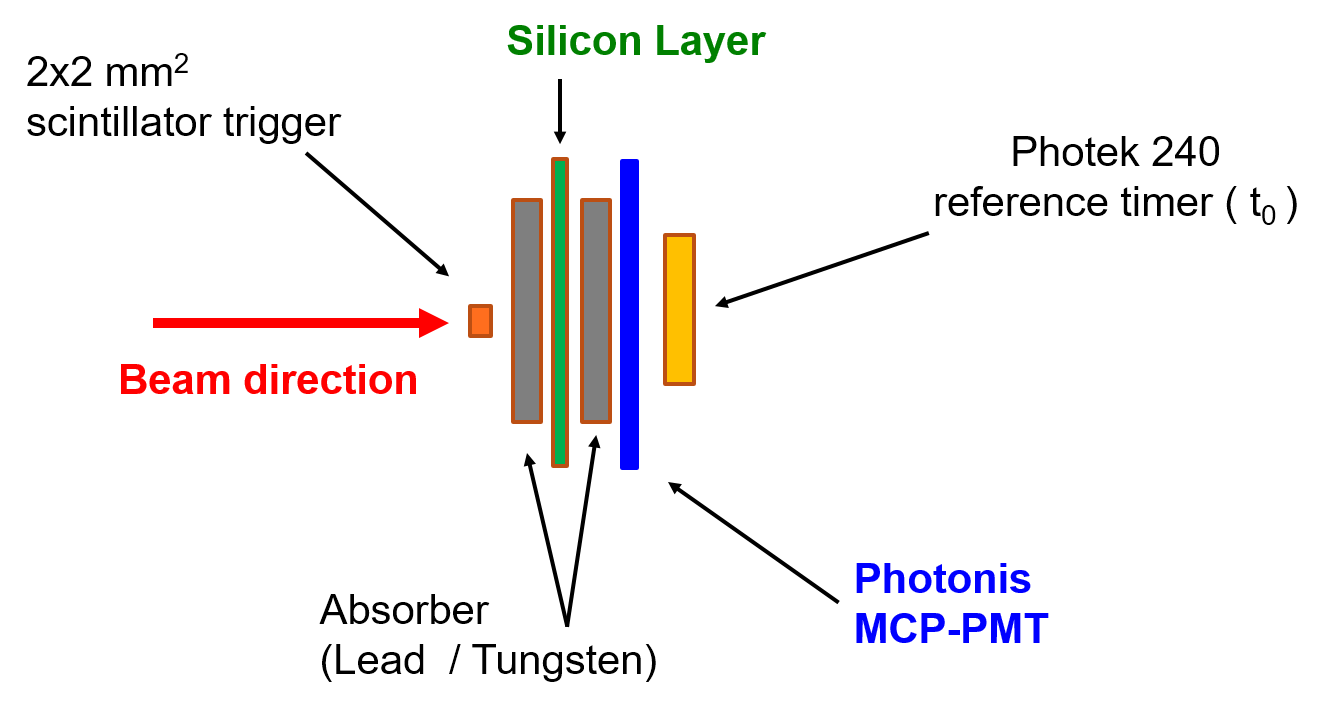
\includegraphics[width=\linewidth]{si_setup.png}
	\caption{A typical experiment configuration.}
	\label{fig:setup}
\end{figure}

The silicon layer combines with the absorber in front of it to simulate an HGC layer, which also has silicon pixel detectors in a hexagonal honeycomb geometry with a layer of tungsten absorber in front \cite{P2}.

A depiction of the HGC layer is given in Figures \ref{fig:silicon-layer} and \ref{fig:HGC}. 
Because the beam is focused at the HGC center pixel (0 in Figure \ref{fig:HGC}), its signal is reduced using a 6 dB attenuator due to the high charge detected relative to other pixels.

\begin{figure}[!htb]
	\centering
	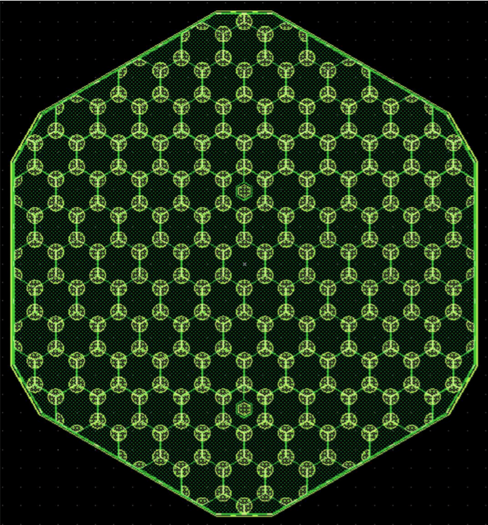
\includegraphics[width=.464\linewidth]{silicon_pixel.png}
	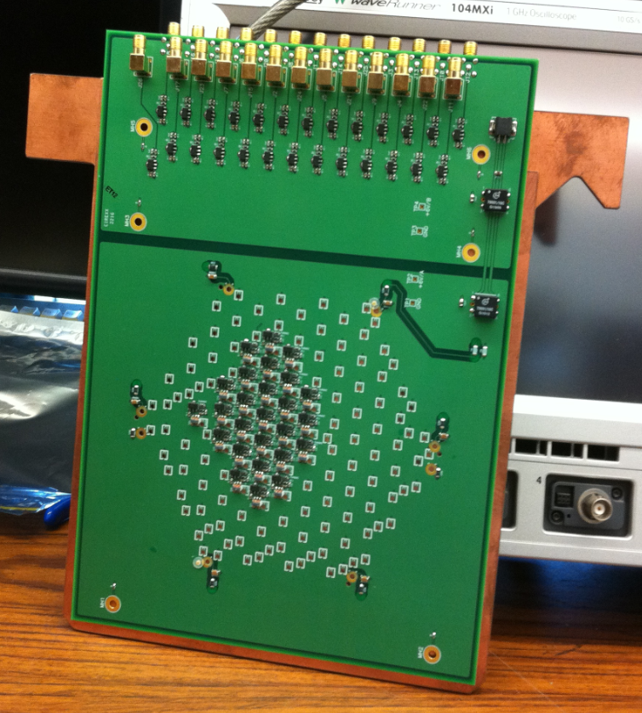
\includegraphics[width=.45\linewidth]{silicon_layer.png}
	\label{fig:silicon-layer}
    \caption{Left: The silicon-based pixel detector \cite{Si_ppt}. 
    Right: The layer comprised of silicon-based pixel detectors \cite{Si_ppt}.}
\end{figure}

\begin{figure}[!htbp]
	\centering
	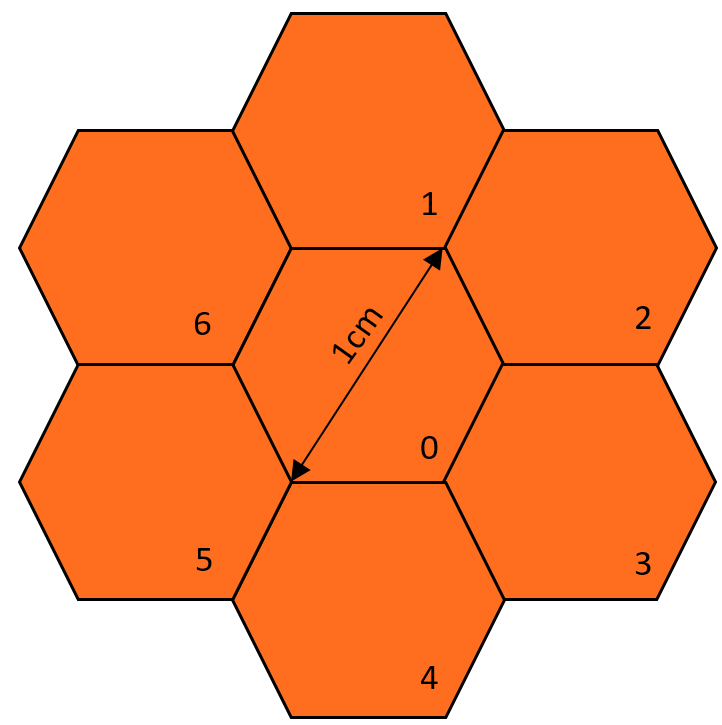
\includegraphics[width=0.57\linewidth]{HGC}
    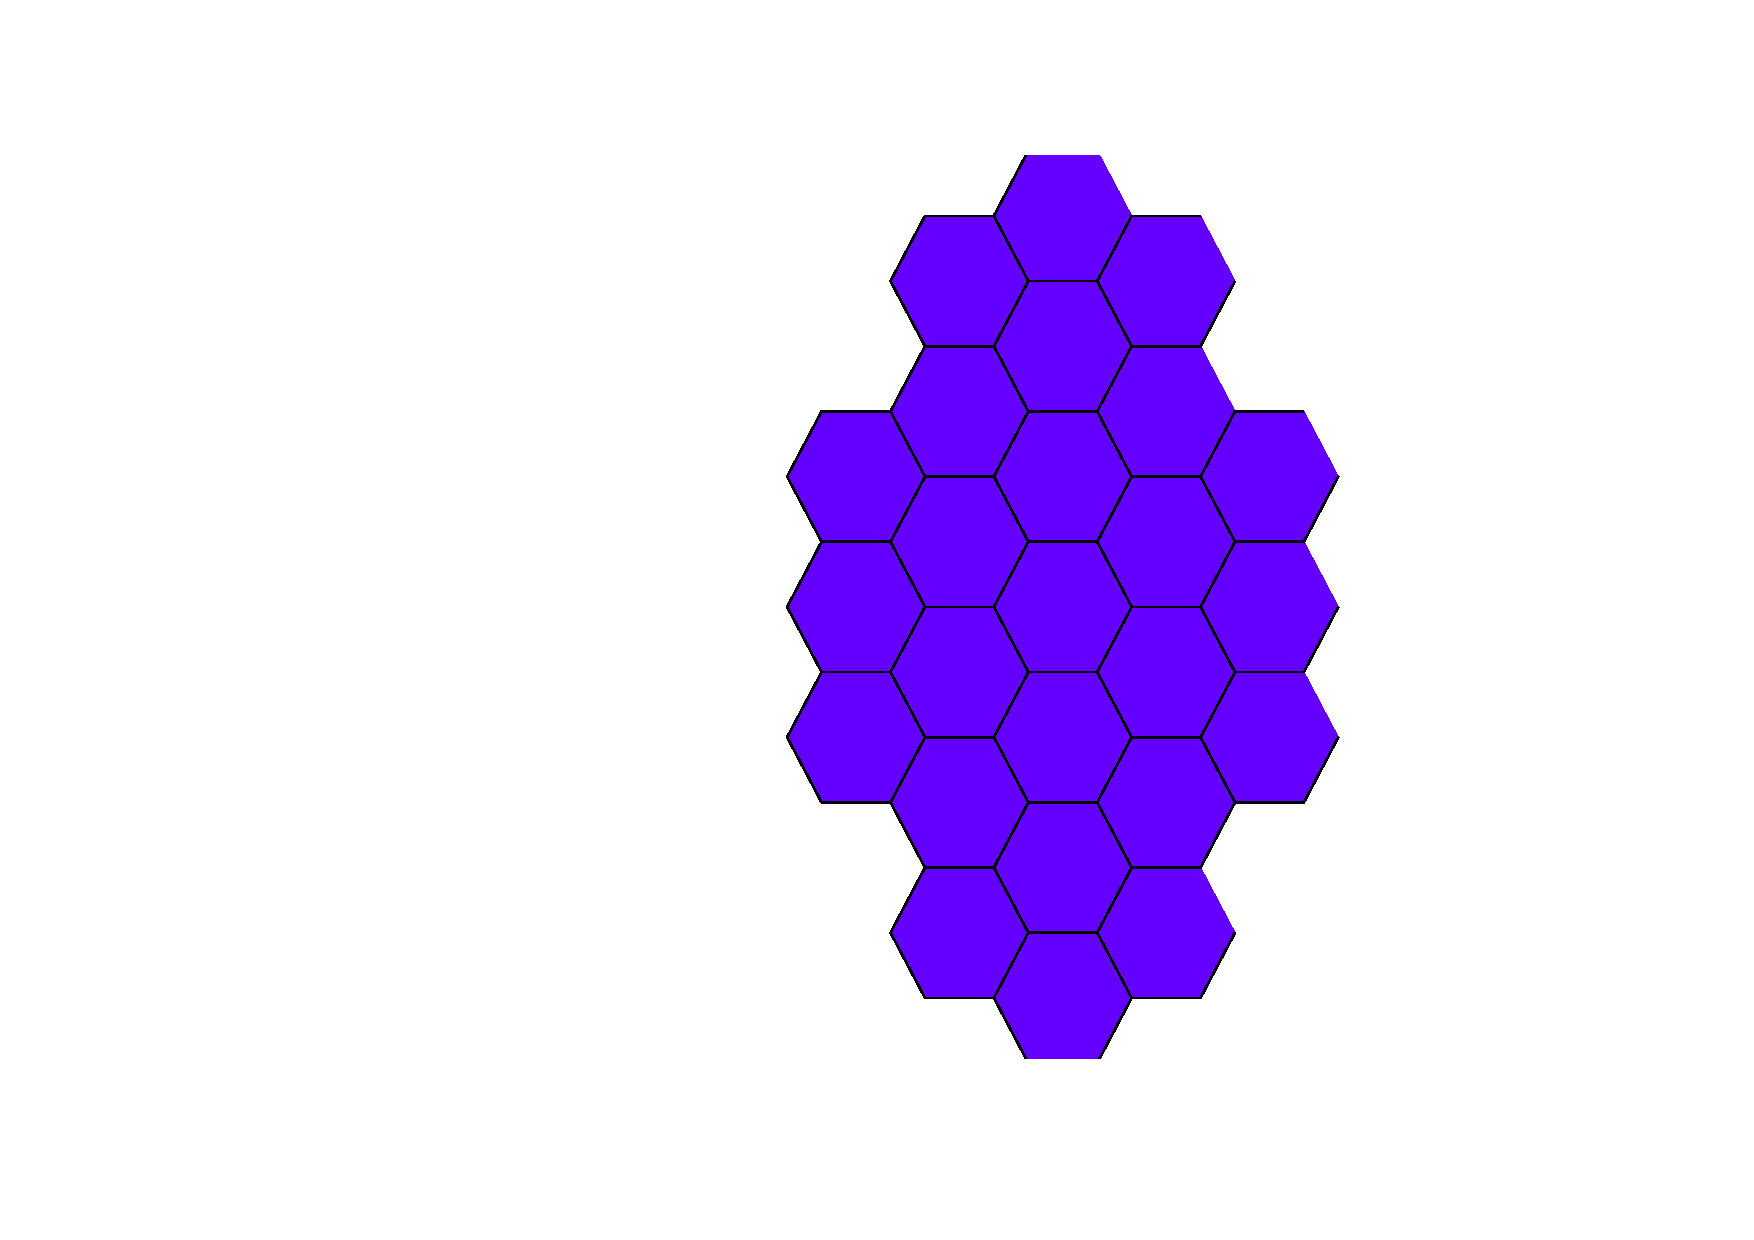
\includegraphics[width=0.37\linewidth]{javier_HGC_plot_--_not_filled_in} 
	\caption{Left: A depiction of the innermost 7 pixels (used for analysis) of the simulated HGC layer. 
	Right: A depiction of the entire simulated HGC layer.}
	\label{fig:HGC}
\end{figure}

In the back, the Photek 240 MCP-PMT in Figure \ref{fig:photek} is used as a reference detector due to its good time resolution ($\sim$10 ps). 
For data acquisition, the DRS4 (Domino Ring Sampler) evaluation board was used in order to optimize the readout.
The DRS4 electronics have a $\sim$4 ps electronic time resolution, 200 ps samplings, and 750 MHz bandwidth.
Figure \ref{DRS4} shows the DRS4 evaluation board.
The DRS4 board is divided into 4 readout groups, which have a time delay between them.
To have a valid base time, the Photek signal is split into 4 cables and plugged into each group as a reference signal. 

\begin{figure}[!htbp]
	\centering
    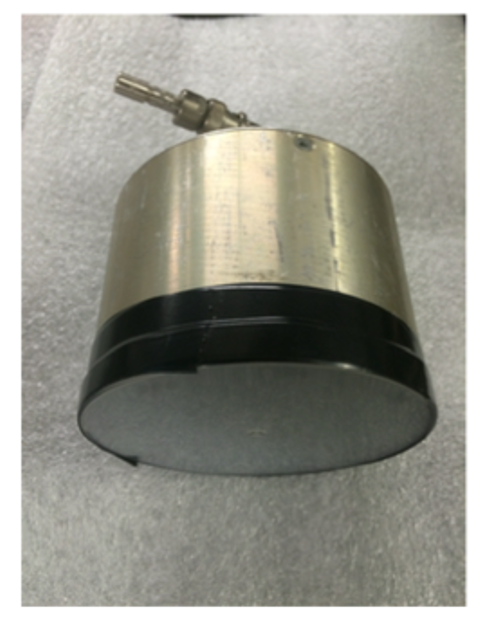
\includegraphics[angle=90,width=.75\linewidth]{photek}
    \caption{The Photek 240 MCP-PMT that is used as a reference detector. It has a rise time of 230 ps and gain of $1\times 10^6$ \cite{Gillian_ppt}.}
    \label{fig:photek}
\end{figure}

\begin{figure}[!htb]
	\centering
	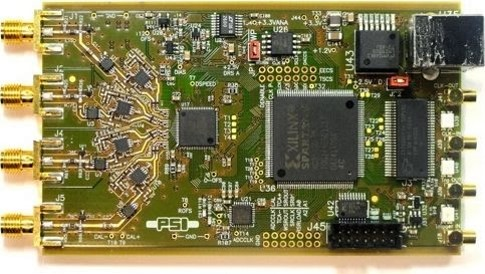
\includegraphics[width=0.9\linewidth]{DRS4_-_Delabs.jpg}
    
    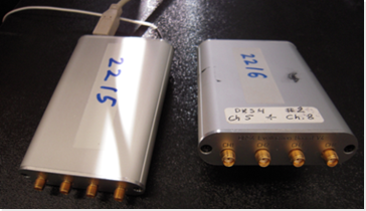
\includegraphics[width=0.9\linewidth]{DRS4}
    \caption{DRS4 evaluation board. Top source: \cite{Si_ppt}. Bottom source: \href{http://www.delabs.net/drs4-evaluation-board-paul-scherrer-institut/}{delabs.net}.}
    \label{DRS4}
\end{figure}

Having a known reference time allows for the TOFs (time of flight, or $\Delta t$) to be calculated. 
The time of flight is the time taken for a particle to travel from a detector to the Photek (used for reference). 
In the data analysis, these TOF values for all events in the run (with certain \textit{bad} events excluded) are combined in a histogram, forming a Gaussian distribution. 
If the jitters/time resolutions on the DRS4 and the Photek are small enough, the $\sigma$ parameter from the distribution \textit{is} the time resolution of the other detector.
However, if the value for $\sigma$ is close to a value for the Photek or DRS4 time resolutions, then the jitter in the Photek/DRS4 is not negligible.
In that case, the DRS4/Photek would increase the $\sigma$ significantly, and the true time resolution of the other detector is less than $\sigma$.

There are a few more detectors in the beam line.
There is a 64-channel and a single-channel Photonis MCP-PMT. 
The 64-channel Photonis was not present for most runs, with the single-channel Photonis being used instead. 
Lastly, a silicon pad (SiPad) detector was present for most runs, however its signal-to-noise ratio was poor, and it does not seem to be useful in most of the analysis.

\section{Data Analysis}
This section aims to explain the general data analysis methods discussed later in this report.

\subsection{Data Analysis: Overview}
The Caltech Precision Timing group already had developed some analysis code for previous test beam experiments, which was updated to handle the idiosyncrasies of this data (e.g. ringing noise). 
The code analyzes the runs and returns a tree with plots and fit results for the pulses (higher-level information).
For example, the values for the pulse height (amplitude) and the pulse integral (charge) for each pulse are returned.
The analysis programs (which output .root files) utilize the ROOT programming language, which is based largely on C++ but contains some additional packages and functionalities. 
ROOT is the main programming language used by scientists at CERN and in the field of HEP (see: \href{root.cern.ch}{root.cern.ch}).

Because the HGC layer has multiple pixels, each pixel detects different signals and has a different time resolution. 
A second analysis code (which should be applied \textit{after} the first) was thus created.
The code calculates the TOF ($\Delta t$) histograms for different pixels, and then combines them in order to return a better overall time resolution. 
The TOF values are calculated for every event in a run by subtracting the pulse time in some device from the pulse time in the Photek (making sure that the device cabling groups --i.e. 1-4-- are the same). 
A 1-D histogram is then populated event-by-event with the TOF values. 
In an ideal world with perfect detectors/readout electronics and no variation in each event, the histogram would be a Dirac delta function with a time resolution of zero. 
However, due to detector jitter, the signal-to-noise ratio and the particle shower development in the material will vary with each event, resulting in Gaussian-distributed TOF histograms \cite{P2}. 
After fitting the histogram to a Gaussian, the $\sigma$ parameter gives the time resolution of the detector/pixel. 
If weighted correctly, combining the values in the HGC pixels' TOF histograms will result in a histogram with better time resolution (smaller $\sigma$). 
This improvement is due to the combination of non-overlapping information about the shower size and development in each of the detectors.

\begin{figure}[!htb]
\centering
\begin{minipage}[t]{\linewidth}
	\centering
	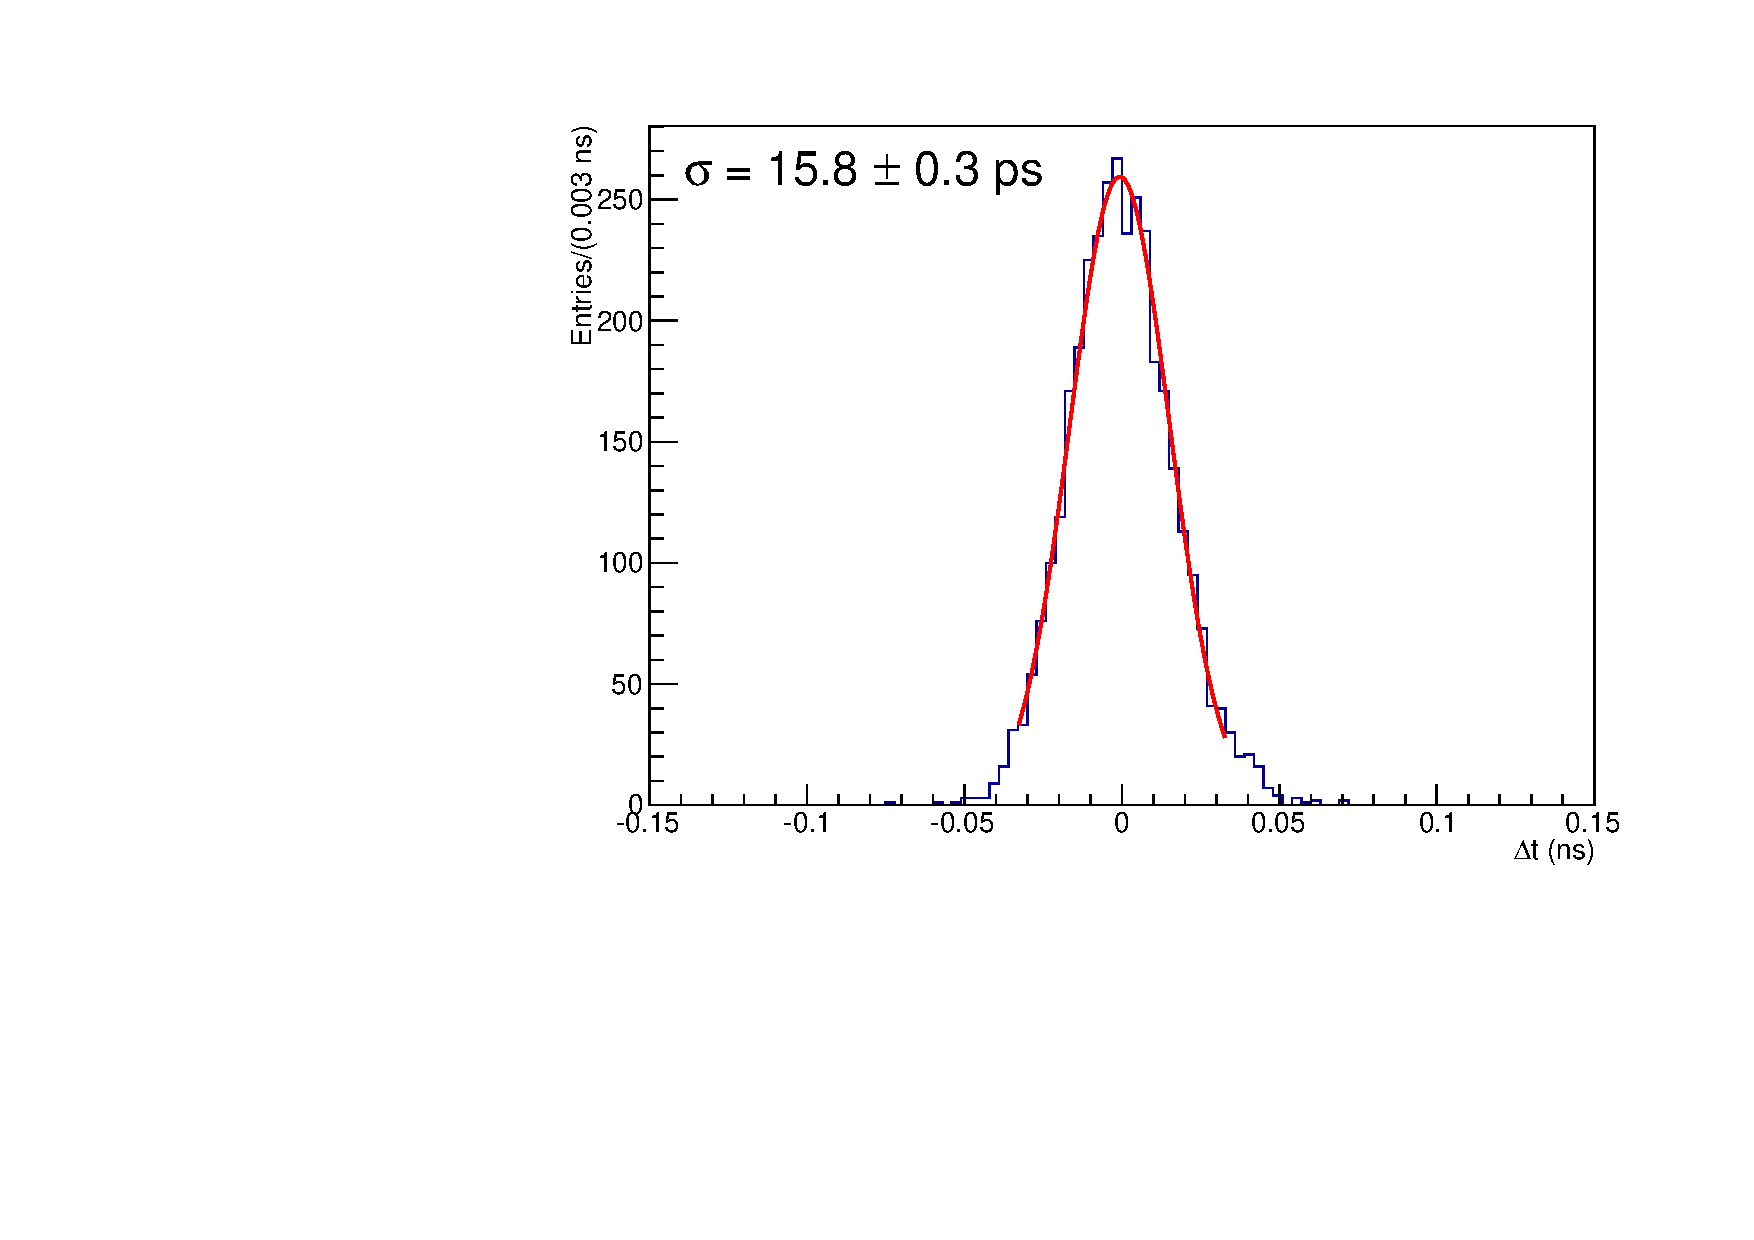
\includegraphics[width=\textwidth]{deltaTCenter.pdf}
	\caption{TOF of the HGC Center Pixel while impinging 32 GeV electrons with 6 $X_0$ Pb in front of the silicon layer.}
	\label{fig:Center}
\end{minipage} \hfill
\newline
\newline
\begin{minipage}[t]{\linewidth}
	\centering
	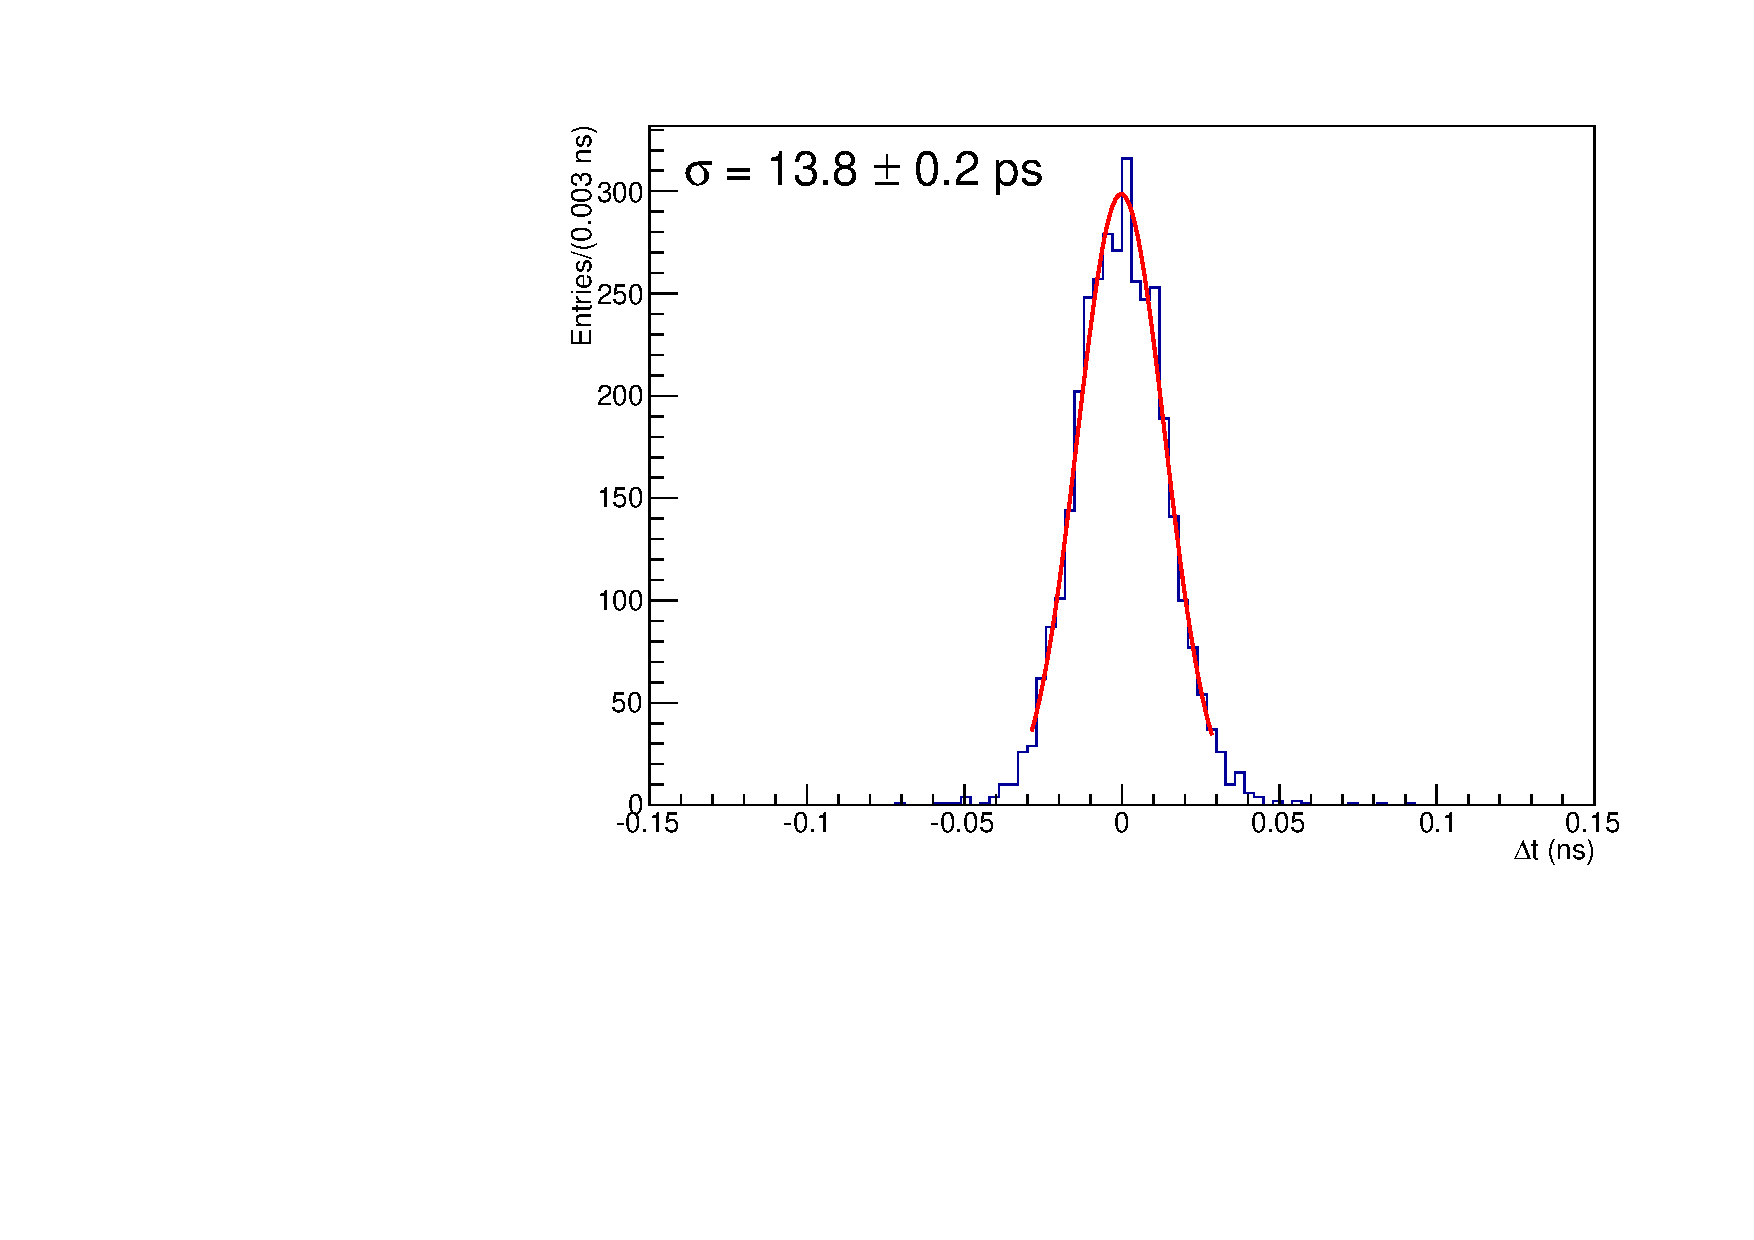
\includegraphics[width=\textwidth]{deltaTMCP.pdf}
	\caption{TOF of the Single-Channel Photonis MCP-PMT while impinging 32 GeV electrons with 6 $X_0$ Pb in front of the silicon layer.}
	\label{fig:MCP}
\end{minipage}
\end{figure}

% The following 2 plots are actually a bit out of date, and were combined with slightly
% different versions of the two above plots. Main point is still correct. Would need to
% update the below plots for any final paper.
\begin{figure}[!htb]
%\centering
%\begin{minipage}[t]{.49\linewidth}
	\centering
	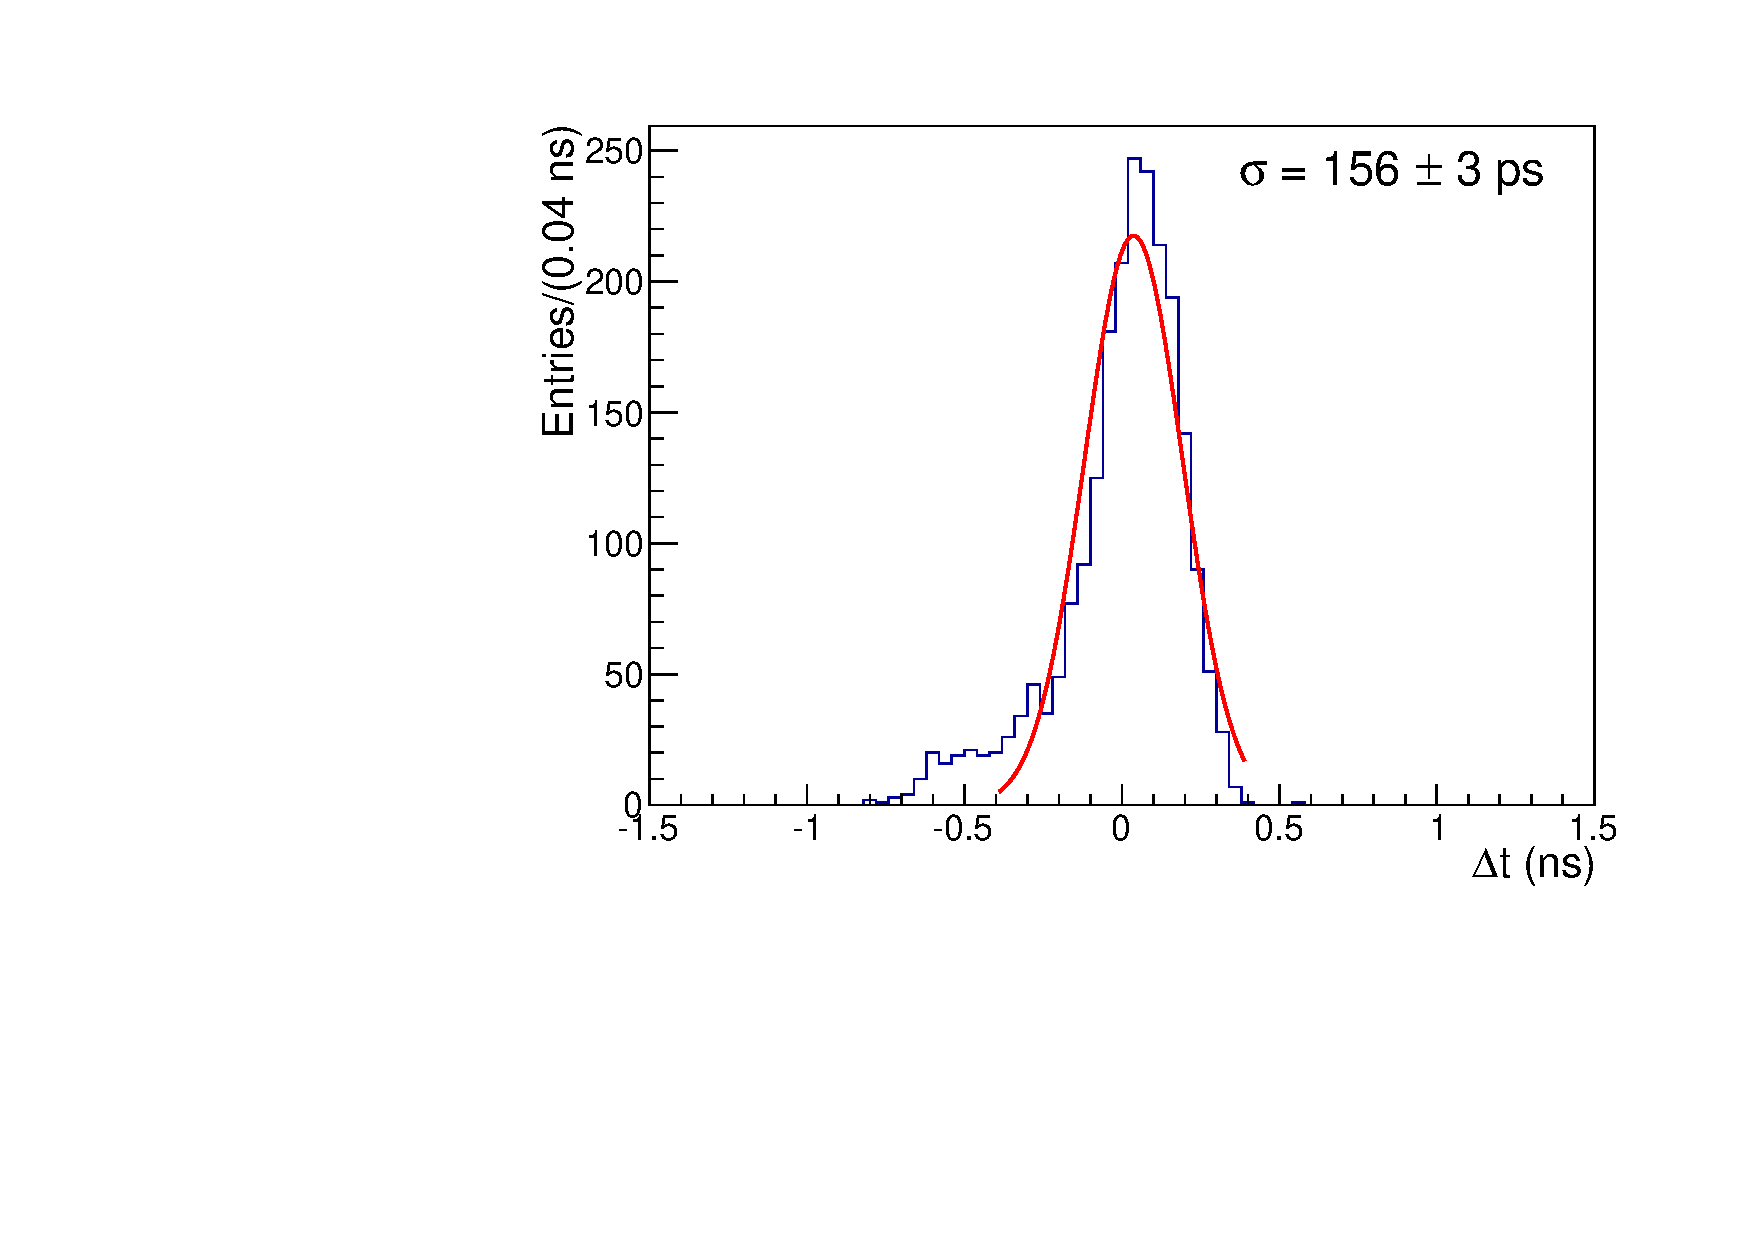
\includegraphics[width=\linewidth]{deltaTSiPad.pdf}
	\caption{TOF of the Silicon Pad while impinging 32 GeV electrons with 6 $X_0$ Pb in front of the silicon layer.}
	\label{fig:SiPad}
%\end{minipage} \hfill
%\begin{minipage}[t]{.49\linewidth}

\centering
	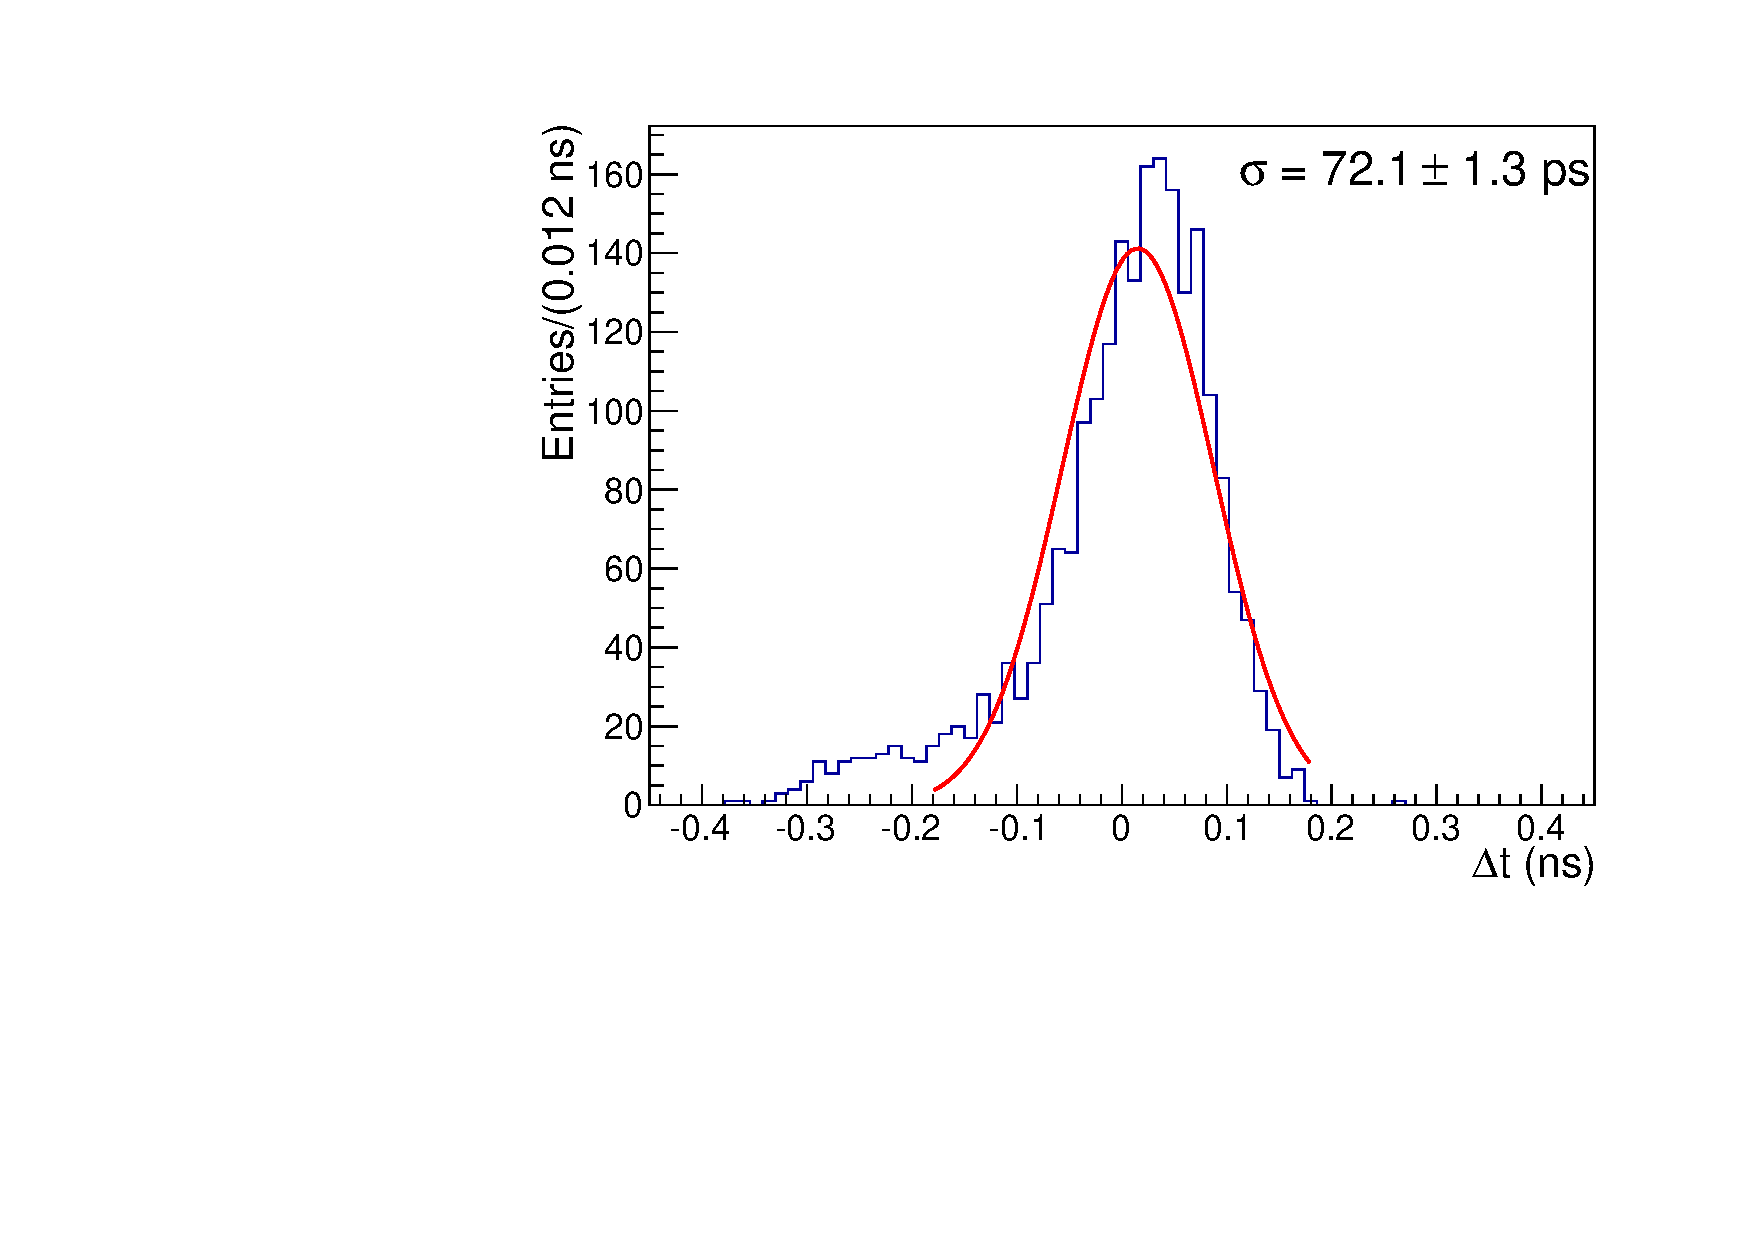
\includegraphics[width=\linewidth]{deltaT_Center_MCP_SiPad_TotalCharge.pdf}
	\caption{TOF of the HGC Center Pixel, Photonis, and Silicon Pad combined using total charge weighting, while impinging 32 GeV electrons with 6 $X_0$ Pb in front of the silicon layer.}
	\label{fig:wctc}
%\end{minipage}
\end{figure}

Because there are also multiple devices along the beam line as well as multiple HGC pixels, the analysis of the coplanar HGC pixels has been called \textit{transverse analysis}, and the analysis of multiple devices \textit{longitudinal analysis}. 
This report shall incorporate both analyses, observing how the time resolution improves with the addition of pixels in the transverse and longitudinal directions.

The silicon pad has noise dominating for most of the runs, and substantially deteriorates the combined detector time resolution. 
For example, Figures \ref{fig:Center} and \ref{fig:MCP} give time of flight ($\Delta t$) histograms for the HGC center pixel and the Photonis MCP-PMT, along with their Gaussian fit $\sigma$ parameter. 
The Gaussian fit utilizes the log-likelihood maximization method, since the $\chi^2$ minimization method is incorrectly biased by histogram bins with few/empty events.
Figure \ref{fig:SiPad} gives the TOF histogram for the silicon pad. 
Figure \ref{fig:wctc} is one possible combination histogram (more details below on how the individual device $\Delta t$'s can be combined). 
Although the combined histogram improves the silicon pad resolution by about 4 times, it is 4-5 times \textit{worse} than the individual resolutions of the HGC or Photonis. 
Additionally, the silicon pad histogram is peaked, but certainly not Gaussian. 
Thus, it is more favorable to simply exclude the silicon pad from the analysis.

Thus, in addition to the HGC layer's center pixel detector, the analysis code will incorporate all of the HGC ring pixels (the 6 pixels surrounding the center pixel; refer to Figure \ref{fig:HGC}) for transverse analysis, as well as the Photonis MCP-PMT for longitudinal analysis.


\subsection{Data Analysis: Event Selection}

\begin{figure*}[!htb]
\centering
	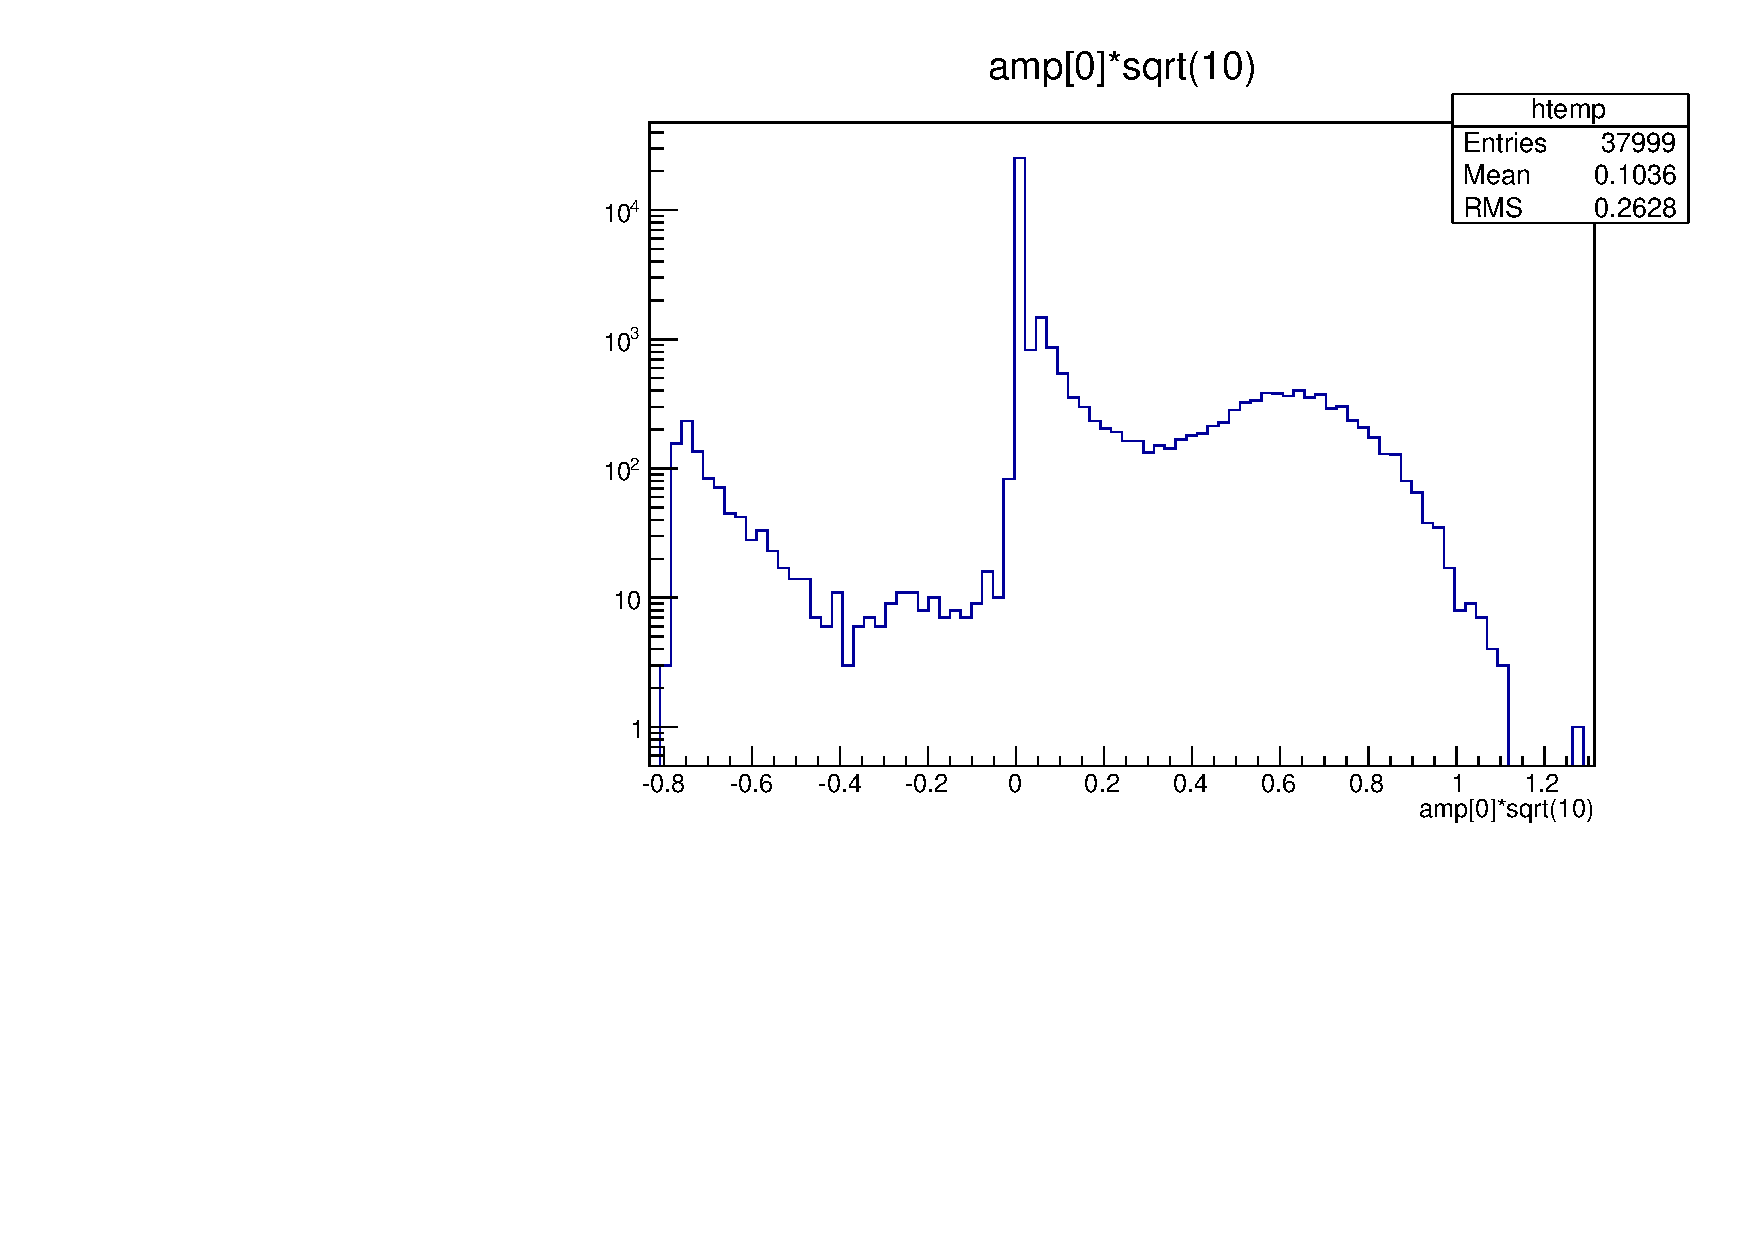
\includegraphics[width=0.49\textwidth]{AmpCut0.pdf}
	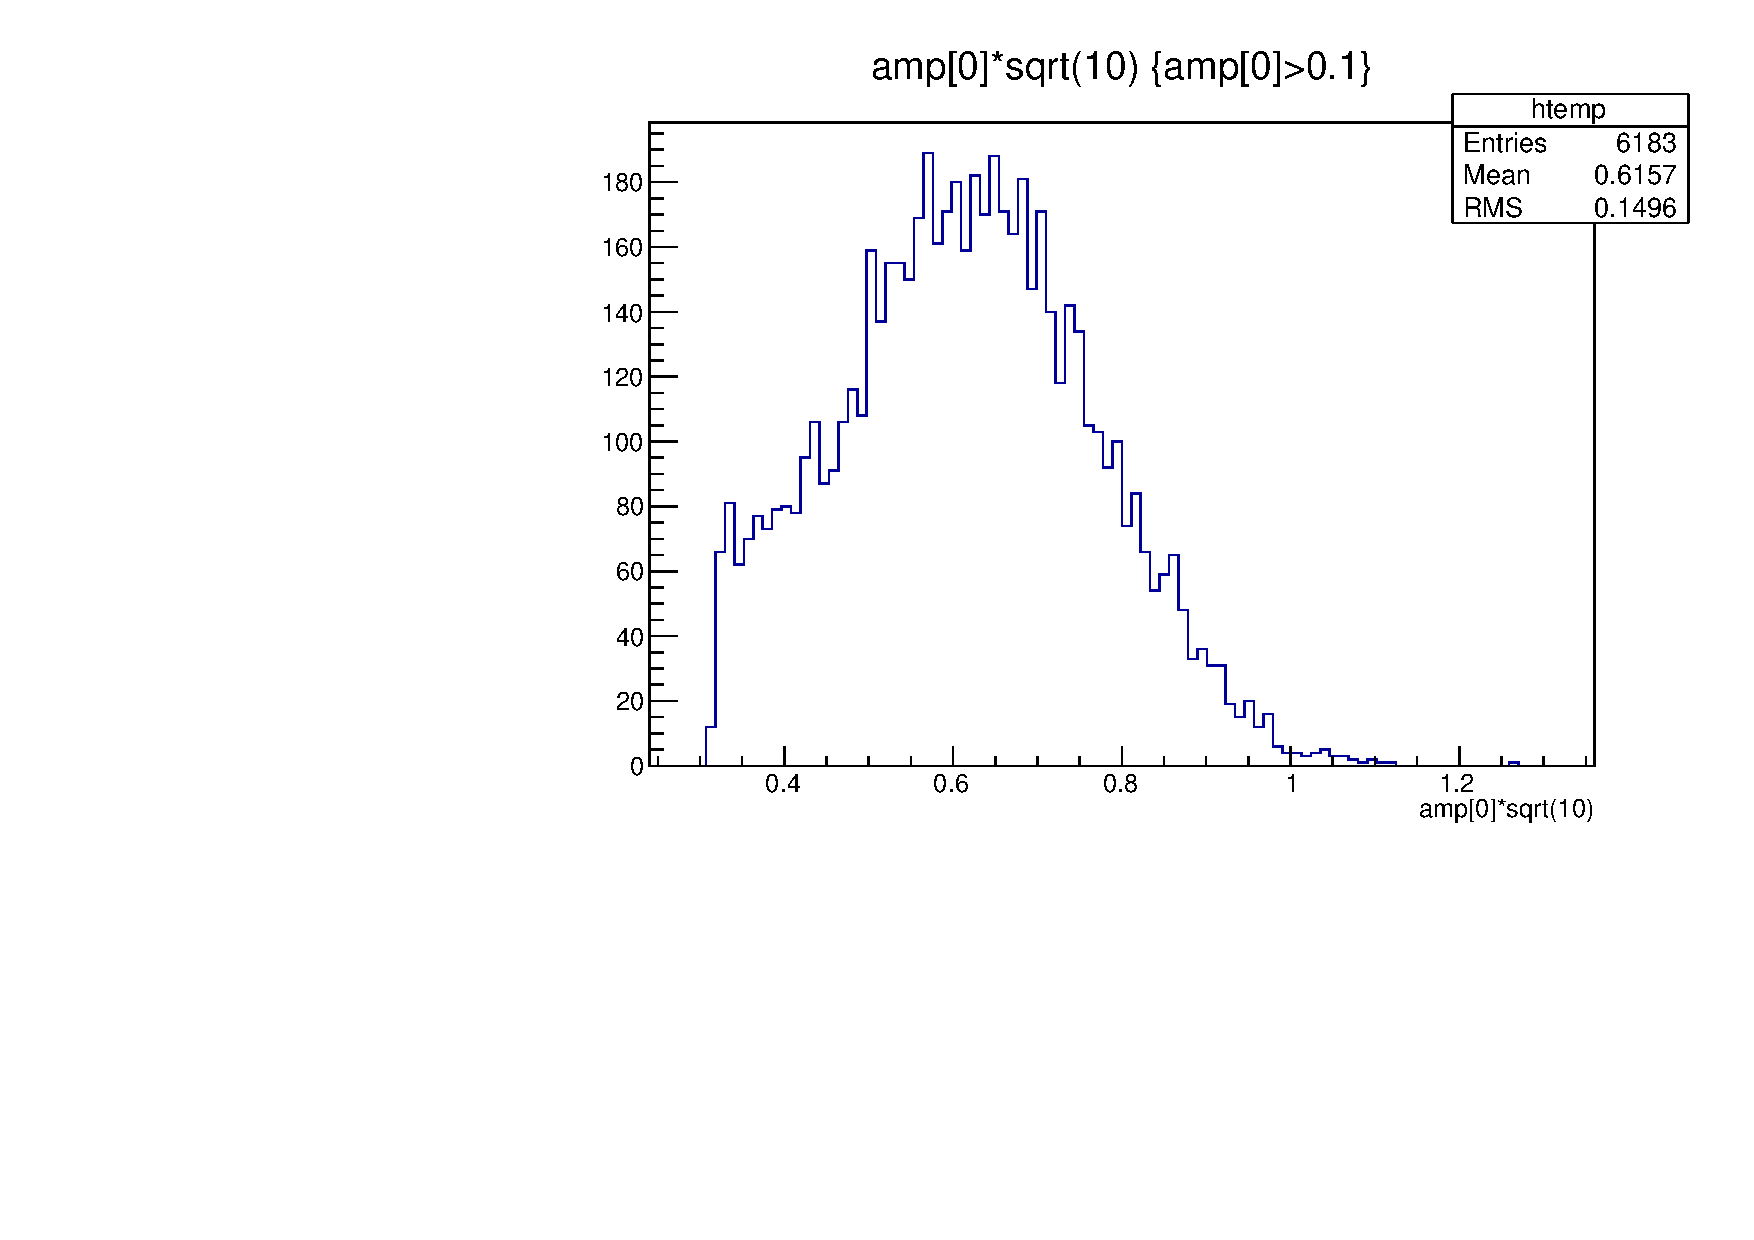
\includegraphics[width=0.49\textwidth]{AmpCut1.pdf}
	\caption{Pulse peak amplitude distribution for the Photek 240 MCP before and after the cut.
		Non-positive amplitudes represent \textit{``bad''} events.
		The $\sqrt{10}$ factor accounts for a 6 dB attenuator.}
	\label{fig:AmpCut}
\end{figure*}

\begin{figure*}[!htb]
\centering
	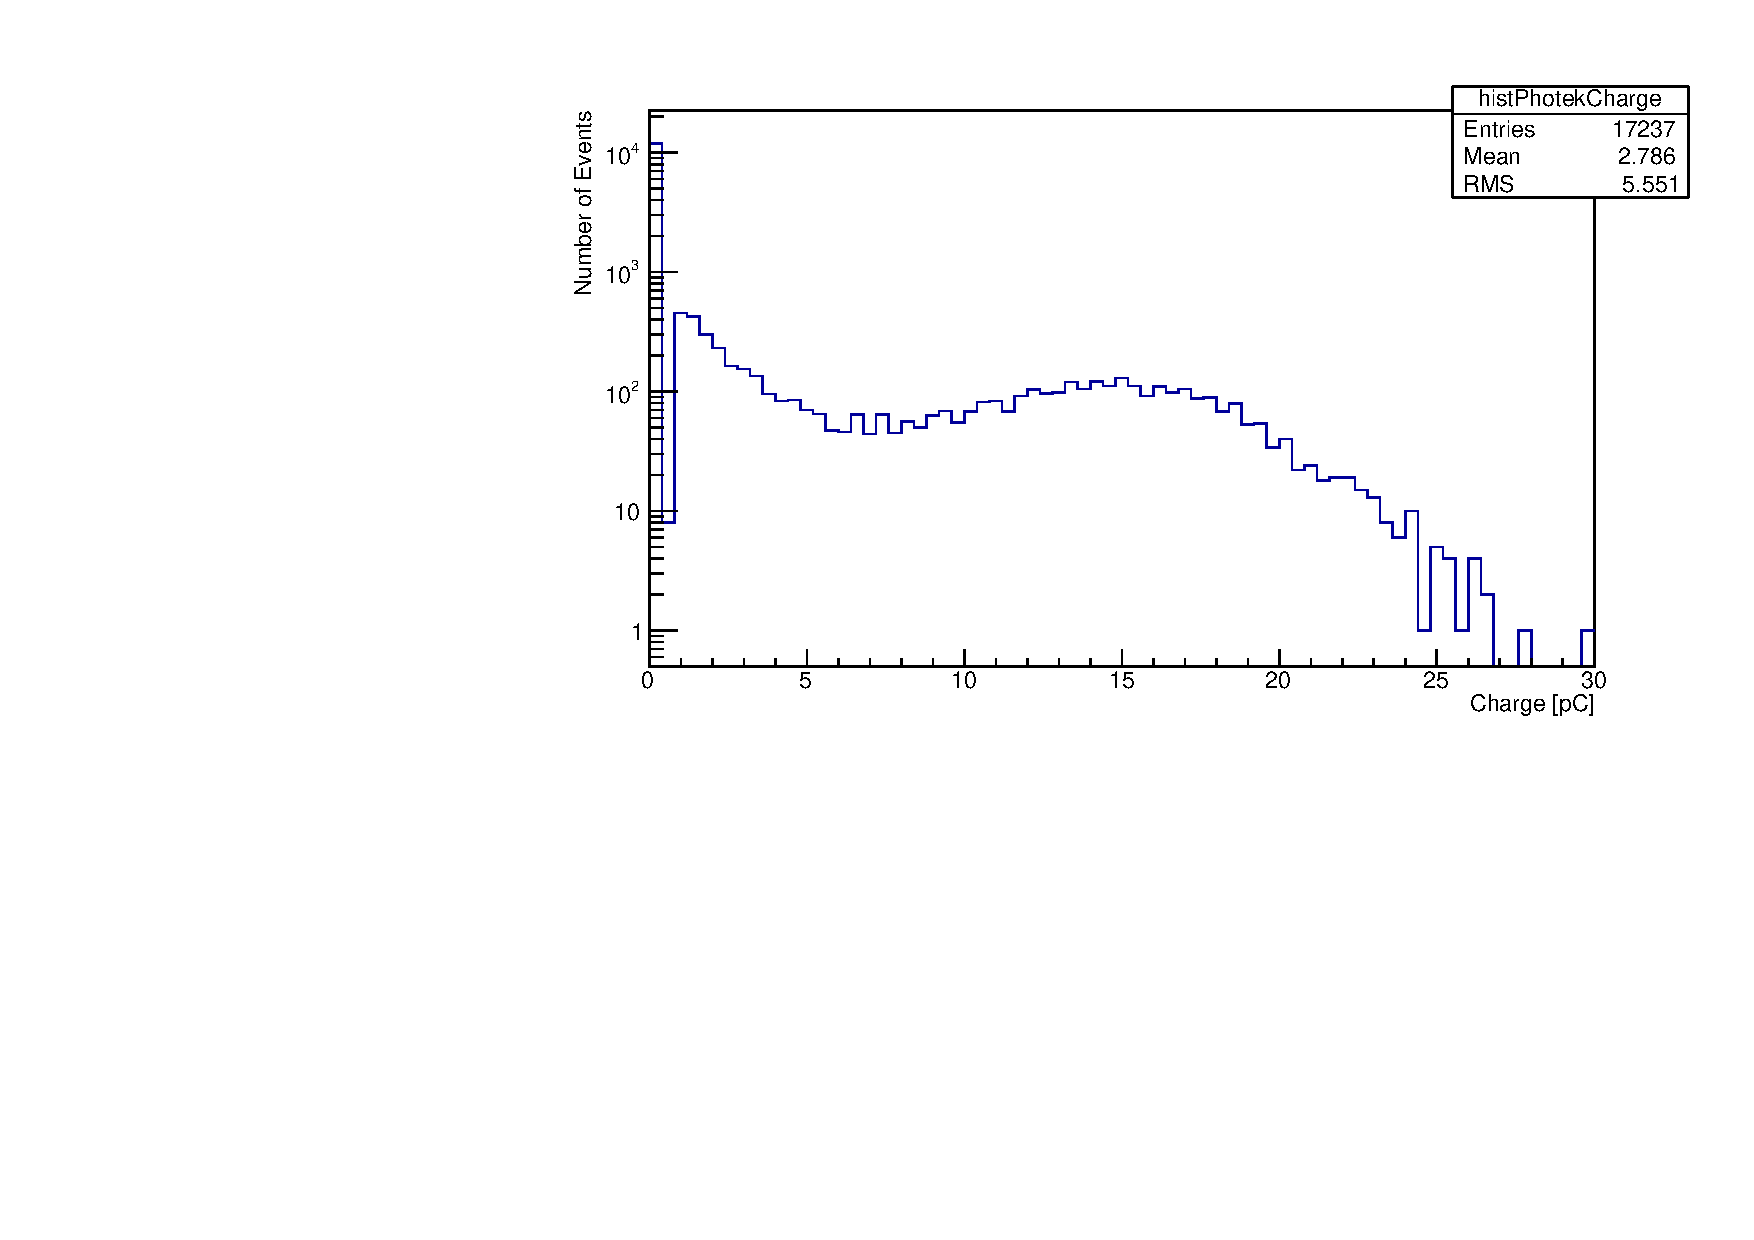
\includegraphics[width=0.49\textwidth]{ChargeCut0.pdf}
	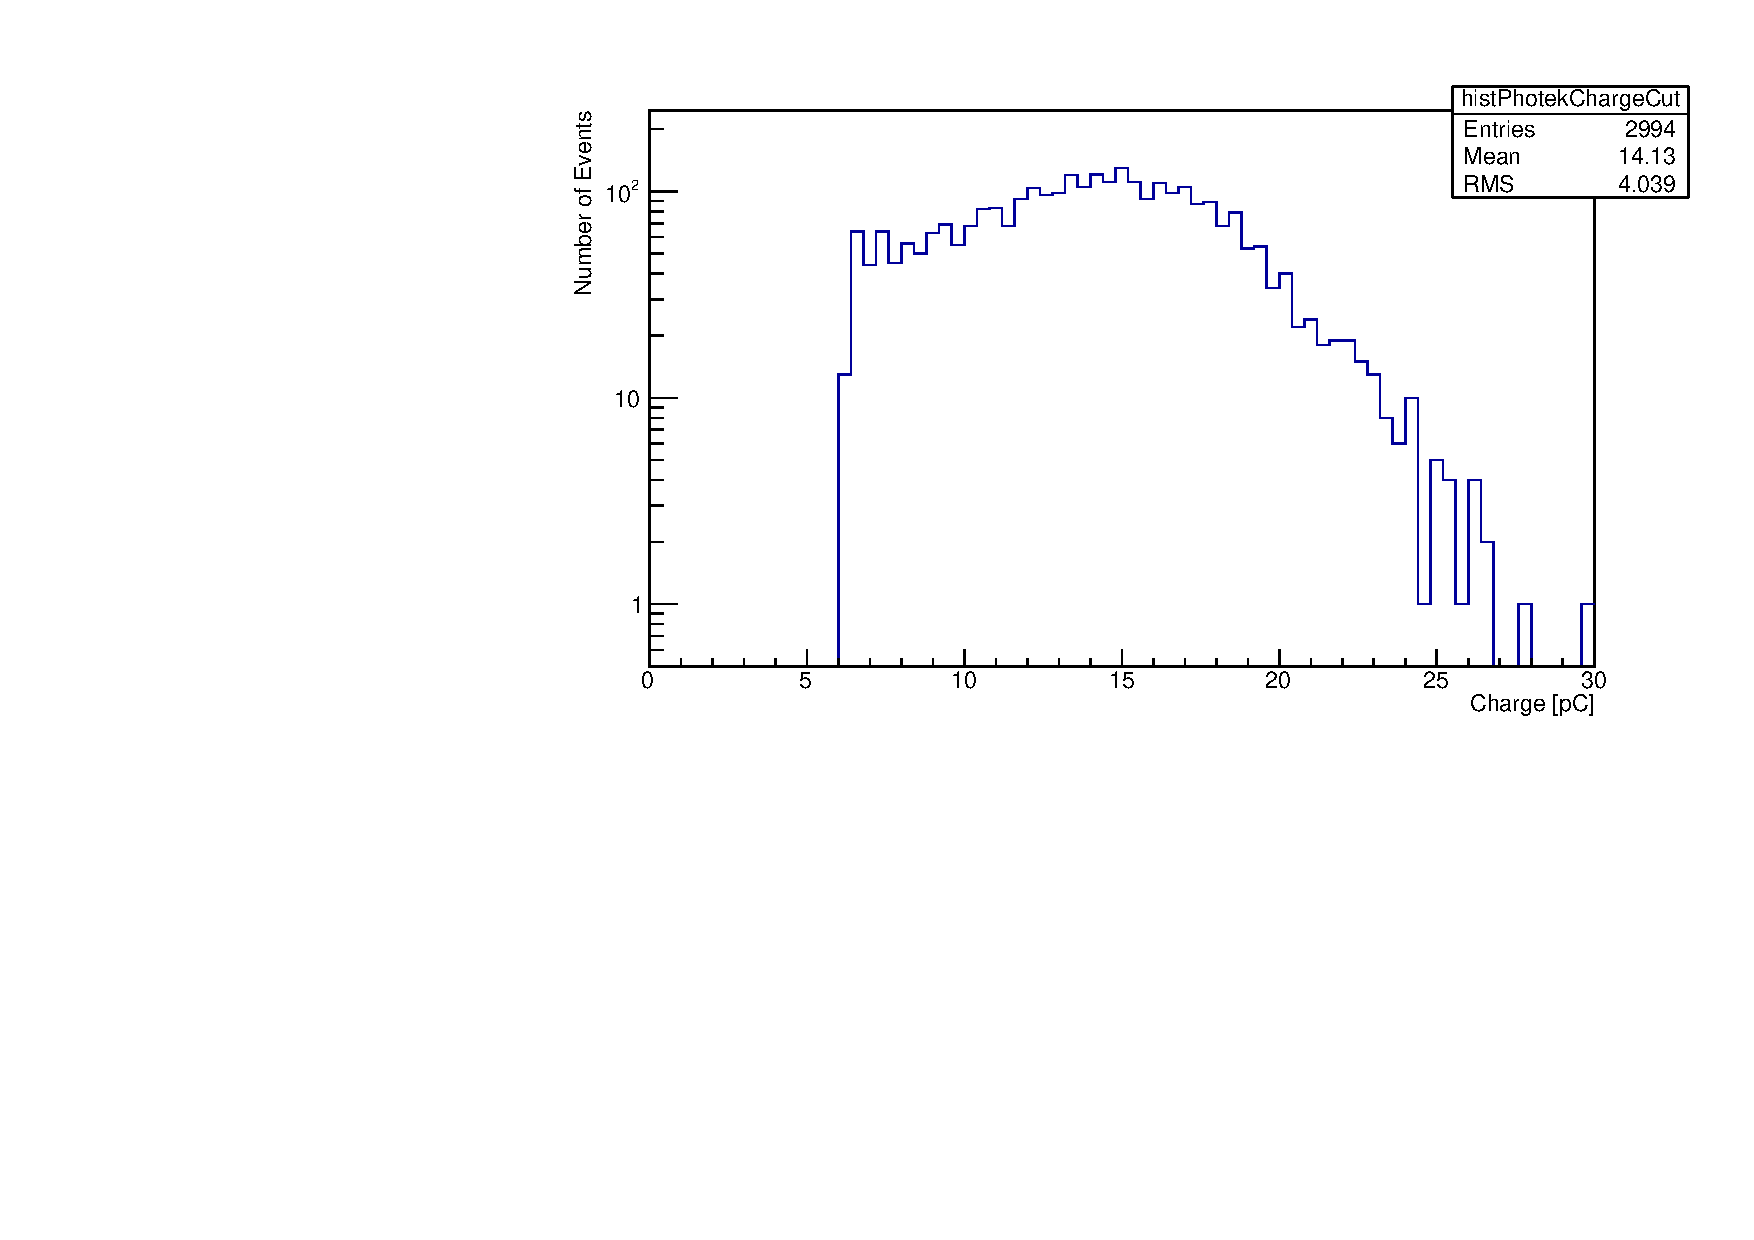
\includegraphics[width=0.49\textwidth]{ChargeCut1.pdf}
	\caption{Pulse charge distribution for the Photek 240 MCP before and after the cut.
		Zeroed charges represent events with only noise.
		The $\sqrt{10}$ factor accounts for a 6 dB attenuator.}
	\label{fig:ChargeCut}
\end{figure*}

Before discussing the various ways to combine the TOF values from different detectors, the methodology for selecting the events that populate the individual device TOF histograms should be reviewed.
Because some events are triggered due to background noise and other events have a lot of ringing noise and a small signal-to-noise ratio, some events need to be excluded from the TOF calculations. 
In order to ensure that most of the \textit{``bad''} events are excluded from the histograms, a cut is applied to the peak amplitude (in mA) and to the overall charge (in pC) of the event, forcing the values to be higher than some threshold. 
This requires that the peak found is not just noise and that the charge is significant enough to represent a pulse.

An example of this event selection is given in Figure \ref{fig:AmpCut}.
Applying the first analysis code returns maximum amplitude values for every event pulse in the Photek. 
Filling a histogram with all of these values gives the left plot in Figure \ref{fig:AmpCut}.
Clearly the non-positive amplitudes are background events or very noisy events. 
These events should be ignored, so a cut is implemented to select for amplitudes above a certain value. 
In this case the value appears to be $0.1\times\sqrt{10}$ mA. 
The right plot in Figure \ref{fig:AmpCut} shows the histogram of the amplitudes with only the events that passed the cut. 
Figure \ref{fig:ChargeCut} shows the same methodology being applied to the charge distribution, with a cut at $2\times\sqrt{10}$ pC. 
Similar cuts were made in the HGC pixels and Photonis MCP-PMT. 

\subsection{Data Analysis: Device Combination}
The second analysis code generates many TOF histograms. 
The simplest are the HGC center pixel and the single-channel Photonis MCP-PMT histograms (Figures \ref{fig:Center} and \ref{fig:MCP}). 
These TOFs are generated from a single detector (without combining other detectors). 
There are 4 main ways that have been utilized to combine different detectors:

\subsubsection{Combination Method: Equal Weighting}
This weighting method is the most straightforward. 
If there are 2 devices which pass the cuts, then their TOF ($\Delta t$) values are computed. 
These 2 TOF values are then combined into a single TOF value by computing the arithmetic average. 
This final TOF is then used to populate the histogram. 
Mathematically, this is given by,
\[
\Delta t_{final} =
\dfrac{\Delta t_1 + \Delta t_2}{2} .
\]

It gets a tad harder to compute $\Delta t_{final}$ when not \textit{all} detectors are required to pass the cuts.
For the HGC layer, many events have 3 or 4 pixels passing cuts, but only a few events have all 7 passing cuts, so the $\Delta t_{final}$ is calculated at every event using whichever pixels were able to pass the cuts. 
This means the number of $\Delta t_{initial}$'s will vary with event. 
Mathematically, it can more generally be written:
\[
\Delta t_{final_i} =
\dfrac{\sum\limits_{k=1}^N \Delta t_{k_i}} {N} 
\]
for N detectors passing cuts, where $\Delta t_{k_i}$ represents the $k^{th}$ detector's TOF at event $i$.

\subsubsection{Combination Method: Event Charge Weighting}
This weighting method uses the detected charge (integral of the pulse) in each device to weight each $\Delta t_{initial}$ value. 
As illustrated in Figure \ref{fig:ChargeCut}, the pulse charge varies with event, so the relative weightings between detectors will change on an event-by-event basis. 
Mathematically, the event charge combination is given by,
\[
\Delta t_{final_i} =
\dfrac{\sum\limits_{k=1}^N \Delta t_{k_i} q_{k_i} }
	{\sum\limits_{k=1}^N q_{k_i} }
\]
for N detectors passing cuts, where $q_{k_i}$ represents the $k^{th}$ detector's charge at event $i$.

\subsubsection{Combination Method: Total Charge Weighting}
Whereas the event charge method weights each detector differently for different events, the total charge method weights each detector the same way over the entire run. 
Rather than use the event charge, this method sums a detector's event charge for every event in the run (i.e. integrating the plot on the right in Figure \ref{fig:ChargeCut}), and uses that value as the weighting factor. 
Mathematically,
\[
\Delta t_{final_i} =
\dfrac{\sum\limits_{k=1}^N \Delta t_{k_i} Q_k }
	{\sum\limits_{k=1}^N Q_k }
,\ \ \ \ 
Q_k = \sum_{all\ events\ i} q_{k_i}
\]
for N detectors passing cuts, where $q_{k_i}$ represents the $k^{th}$ detector's charge at event $i$.

\begin{figure}[!htbp]
	\centering
	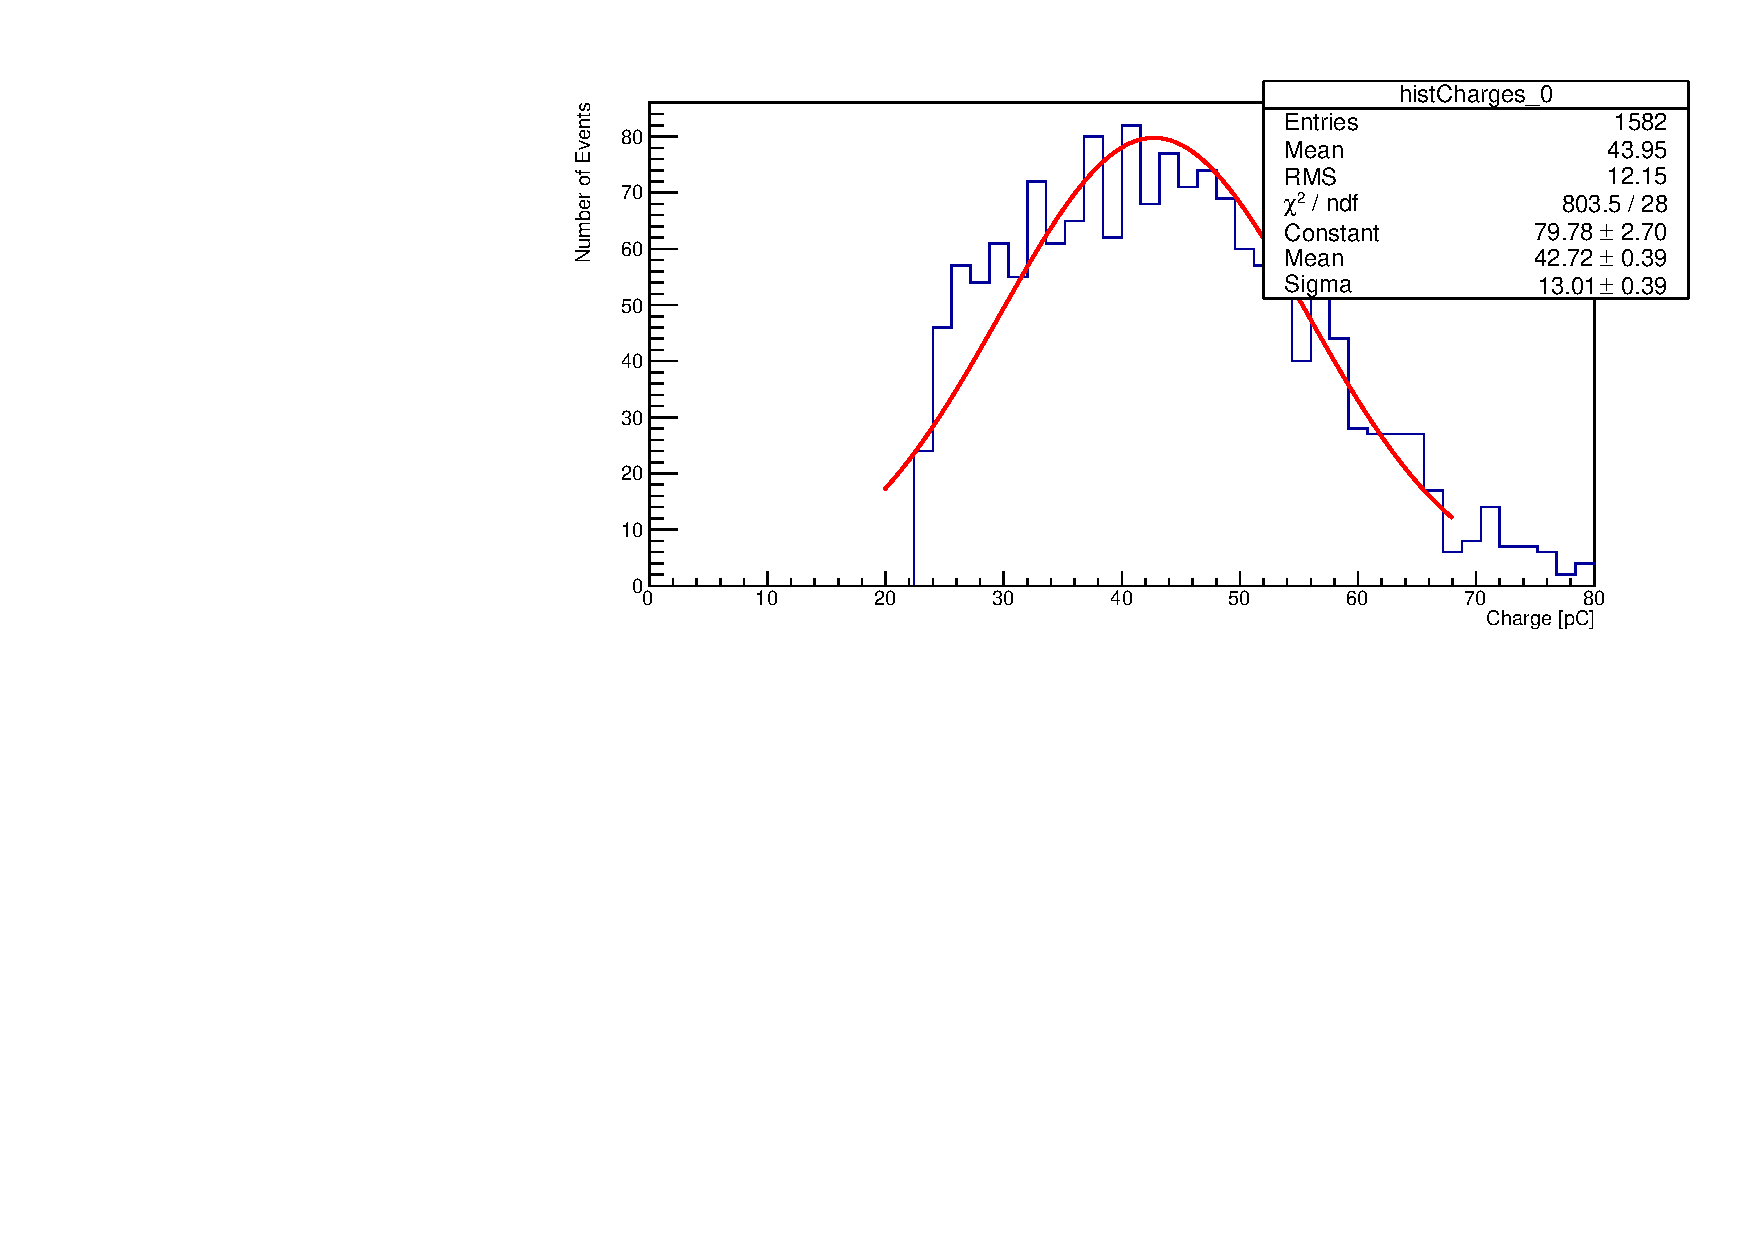
\includegraphics[width=\linewidth]{mpvgaus.pdf}
	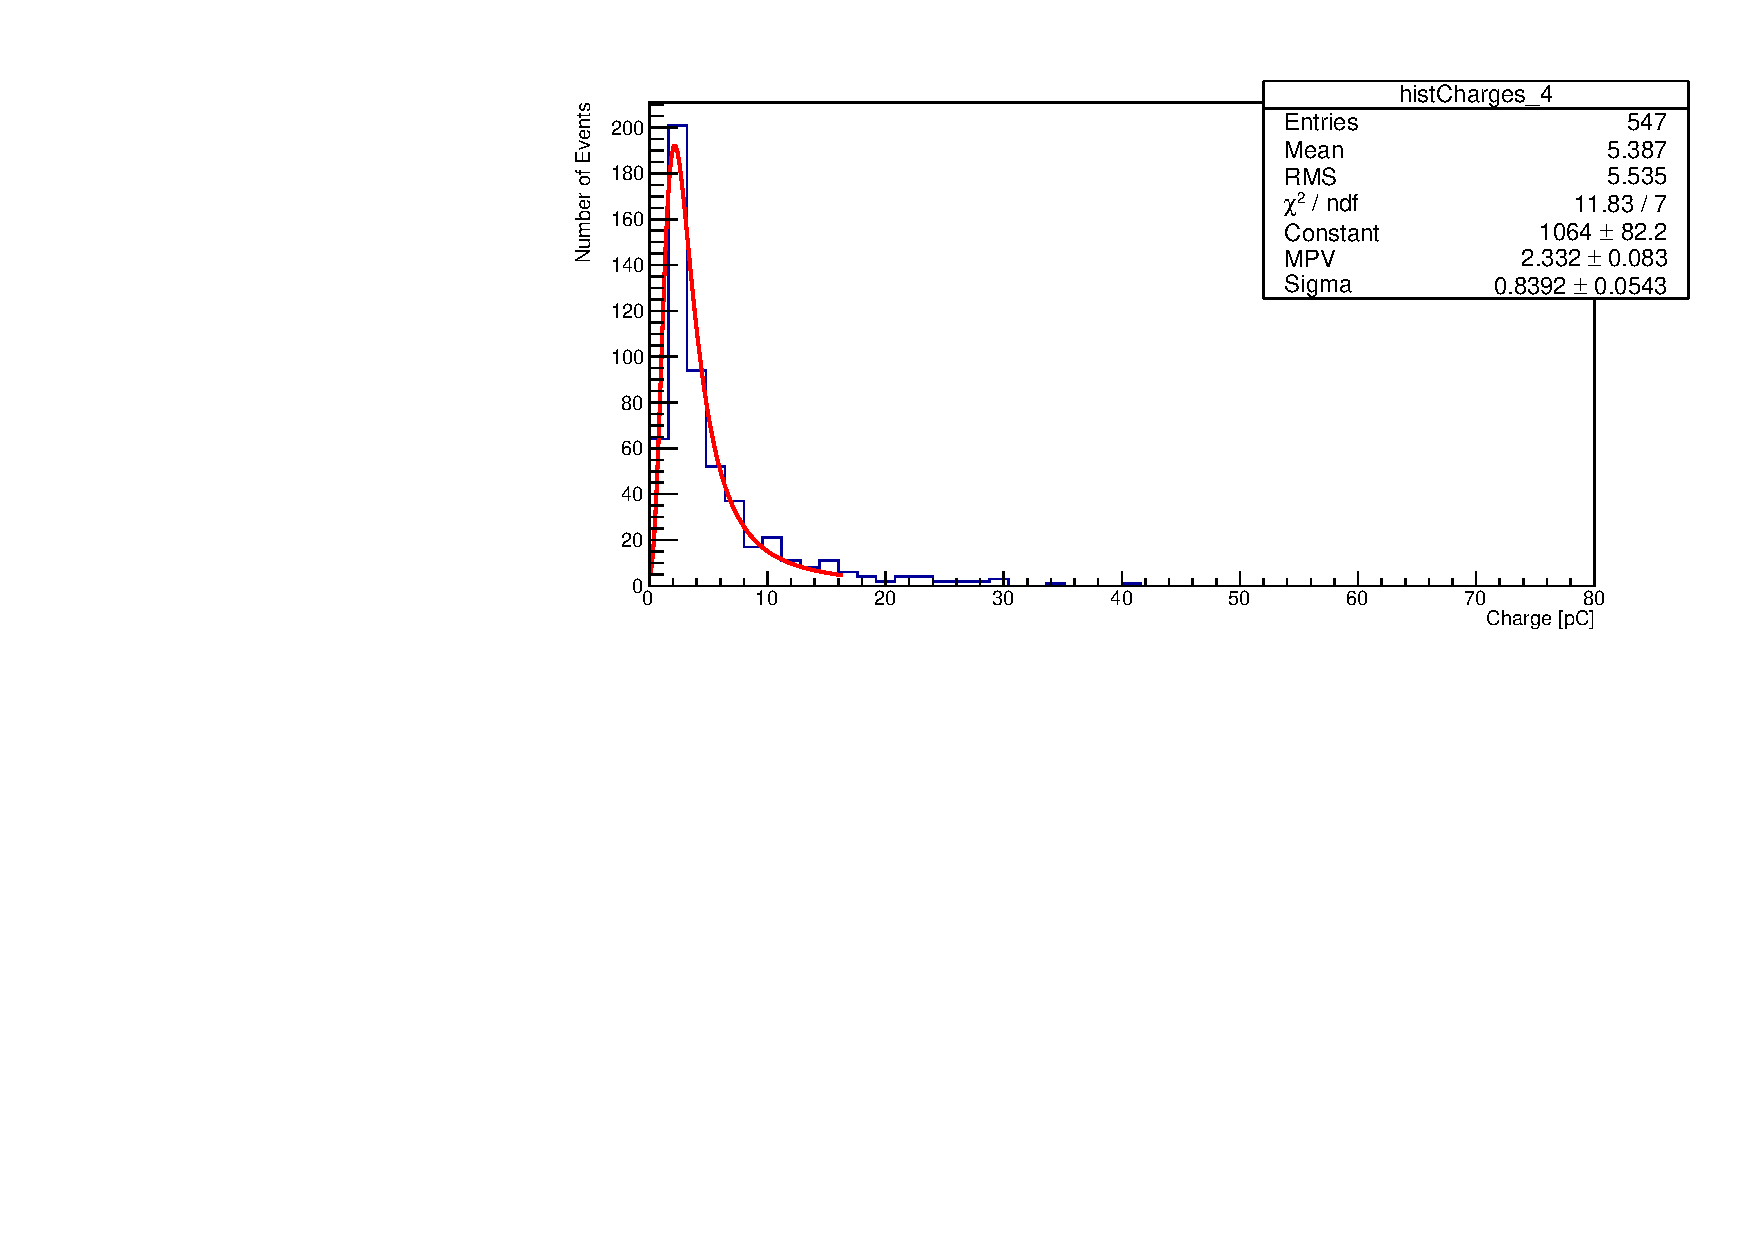
\includegraphics[width=\linewidth]{mpvlandau.pdf}
	\caption{The HGC center pixel's (top) and typical ring pixel's (bottom) charge distribution \textit{after} the cut, overlaid with a Gaussian (top) and Landau (bottom) fit.}
    \label{fig:MPV}
\end{figure}

\subsubsection{Combination Method: Charge MPV Weighting}
Like the total charge method, this method also assigns weighting factors to each detector that do not change with the event. 
Additionally, this method is only used within the HGC layer, for combining the TOFs of different pixel detectors. 
Rather than being determined by the total charge detected, this method fits a Landau distribution to the charge distribution histogram of each of the 6 ring pixels.
The peak, or most probable value (MPV), of the fit is then used as the weighting factor for the ring pixels. 
Figure \ref{fig:MPV} gives examples of these fits.
Because there are far more events passing cuts -- and with a higher charge -- in the center pixel, the distribution is described better by a Gaussian, and its weighting factor is the mean $\mu$ of a Gaussian fit.
Both types of fits are accomplished by maximizing the log-likelihood in order to avoid the biasing of the $\chi^2$ minimization fit for low-event bins.
Mathematically, this method is represented by the same formula as the total charge method, but letting $Q_k$ represent the detector's MPV, instead of total charge.


\section{Time of Flight Plots: Simple Combinations}
Now that all the different combination methods have been described, understanding the resultant plots is possible. 
In order to show results in the simplest manner, this section will only use plots coming from 1 data set with the same configuration. 
Specifically, the results in this section will all be for runs that have a 32 GeV electron test beam, and a tungsten (W) absorber 1mm in front of the HGC layer (it may help to recall the setup from Figure \ref{fig:setup}).

Starting with the more basic (low-level) plots, Figure \ref{fig:center_MCP_104} contains the TOF histograms for the HGC center pixel and Photonis MCP-PMT.

\begin{figure*}%[h]
\centering
	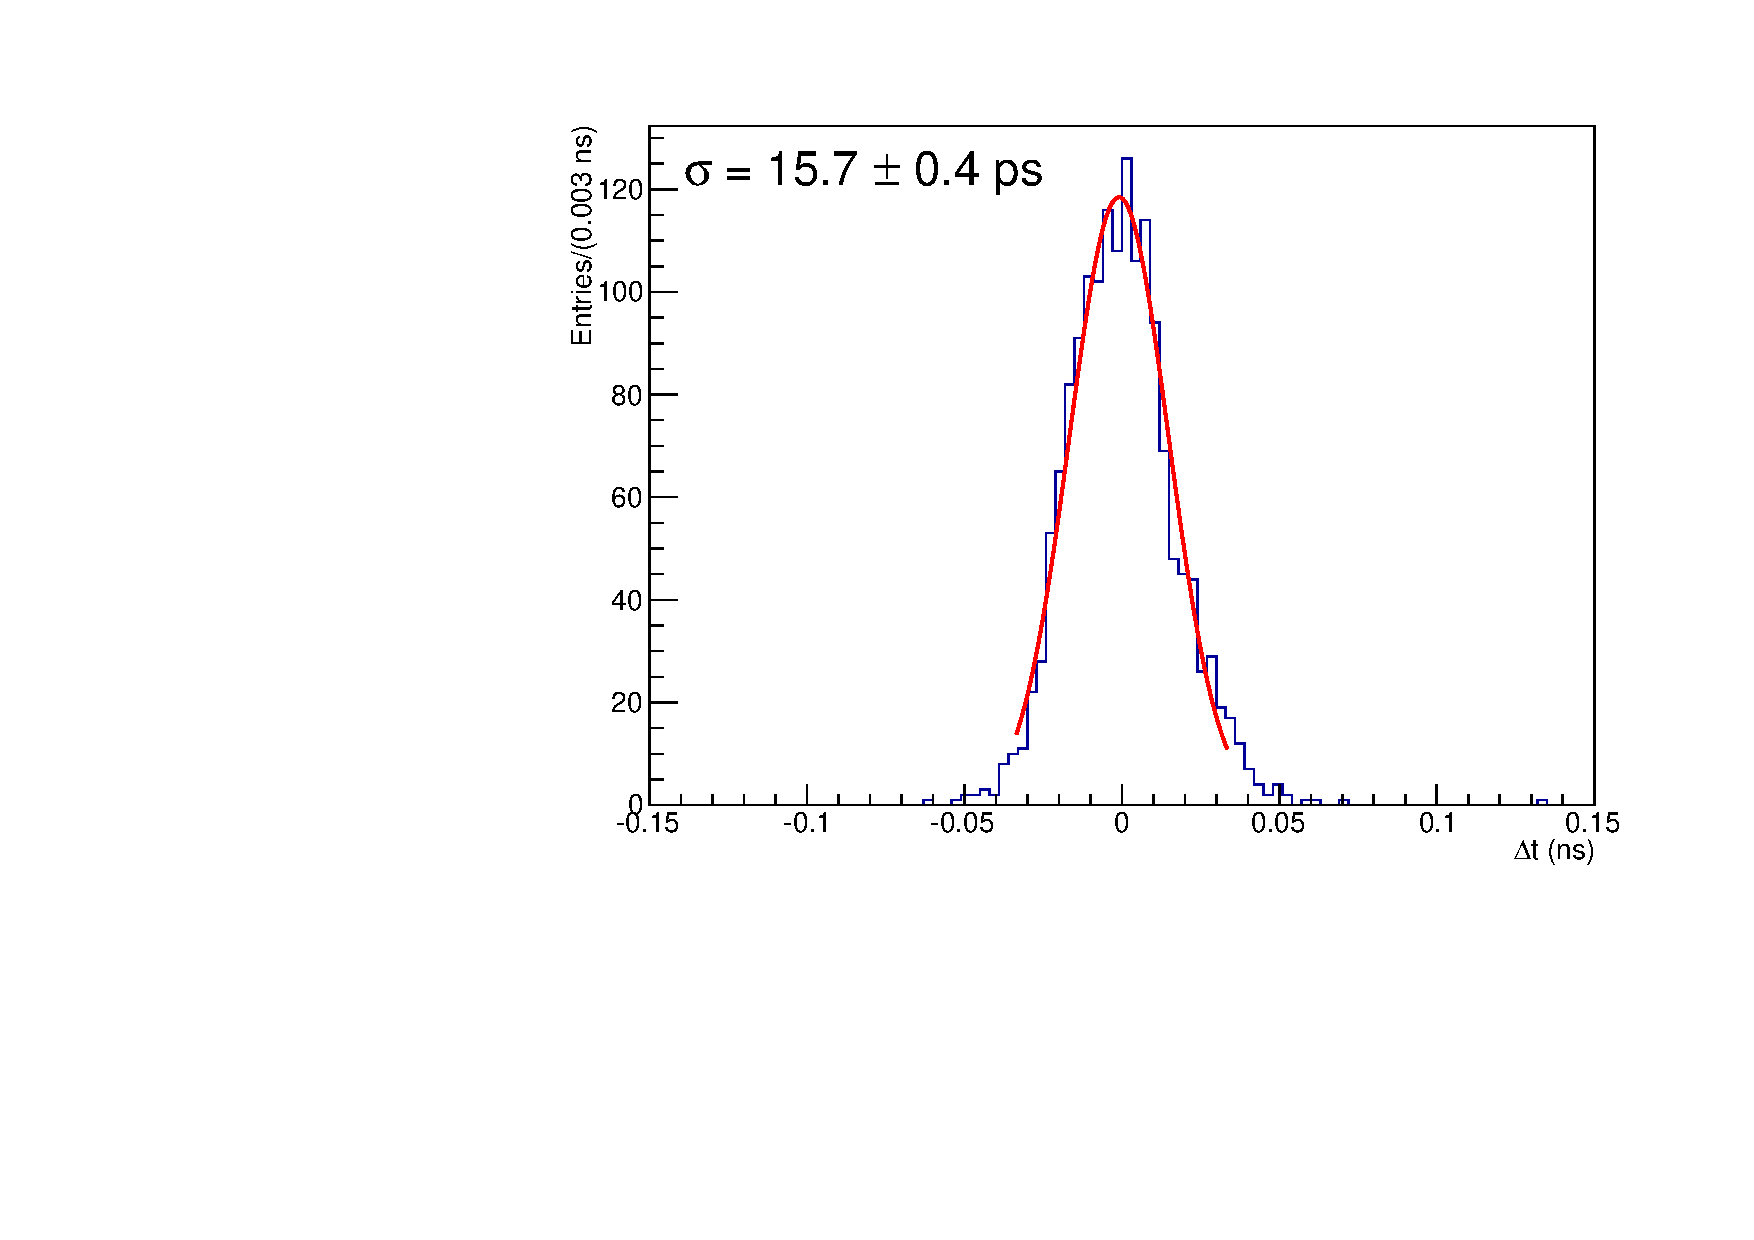
\includegraphics[width=.49\textwidth]{deltaTCenter104.pdf}
	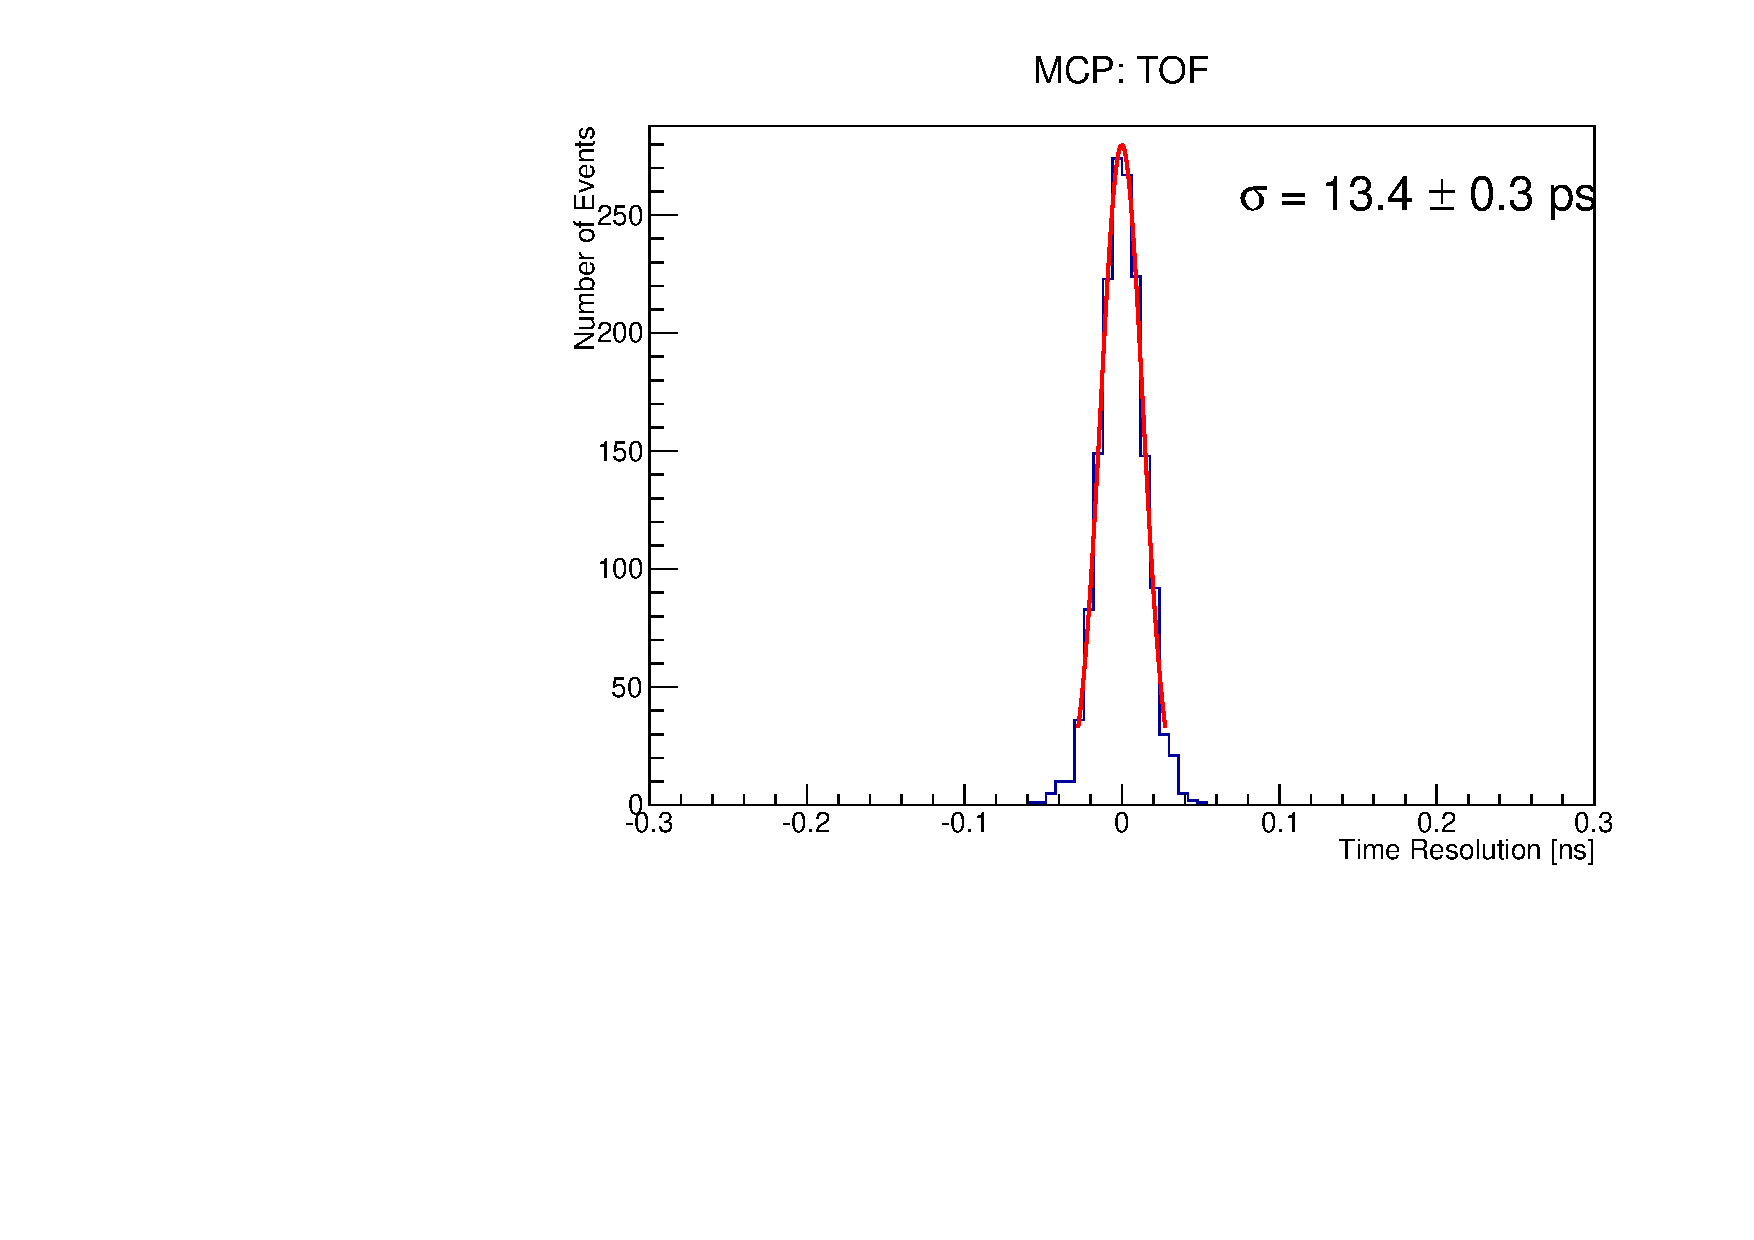
\includegraphics[width=.49\textwidth]{deltaTMCP104.pdf}
	\caption{TOF histograms of HGC center pixel and of Photonis MCP-PMT.}
	\label{fig:center_MCP_104}
\end{figure*}

In order to see how the time resolution improves when adding in the ring pixels, Figure \ref{fig:HGC_event_total_MPV_104} contains different charge-based weighting methods. 
Equal weighting is not used here because the center pixel has more events and a better time resolution than the other pixels, so it should be weighted more heavily. 
The center pixel has a better time resolution because the beam is focused on it, which increases the number of events and thus the signal-to-noise ratio. 
For all combinations in Figure \ref{fig:HGC_event_total_MPV_104} there is a decrease in $\sigma$ (from 15.9 ps in Figure \ref{fig:center_MCP_104}) and thus an improvement in the time resolution. 
Although the uncertainties in $\sigma$ are too large to be conclusive here, Figure \ref{fig:HGC_event_total_MPV_104} suggests that the event charge weighting is the worst of the 3 methods.

\begin{figure*}[!htbp]
\centering
	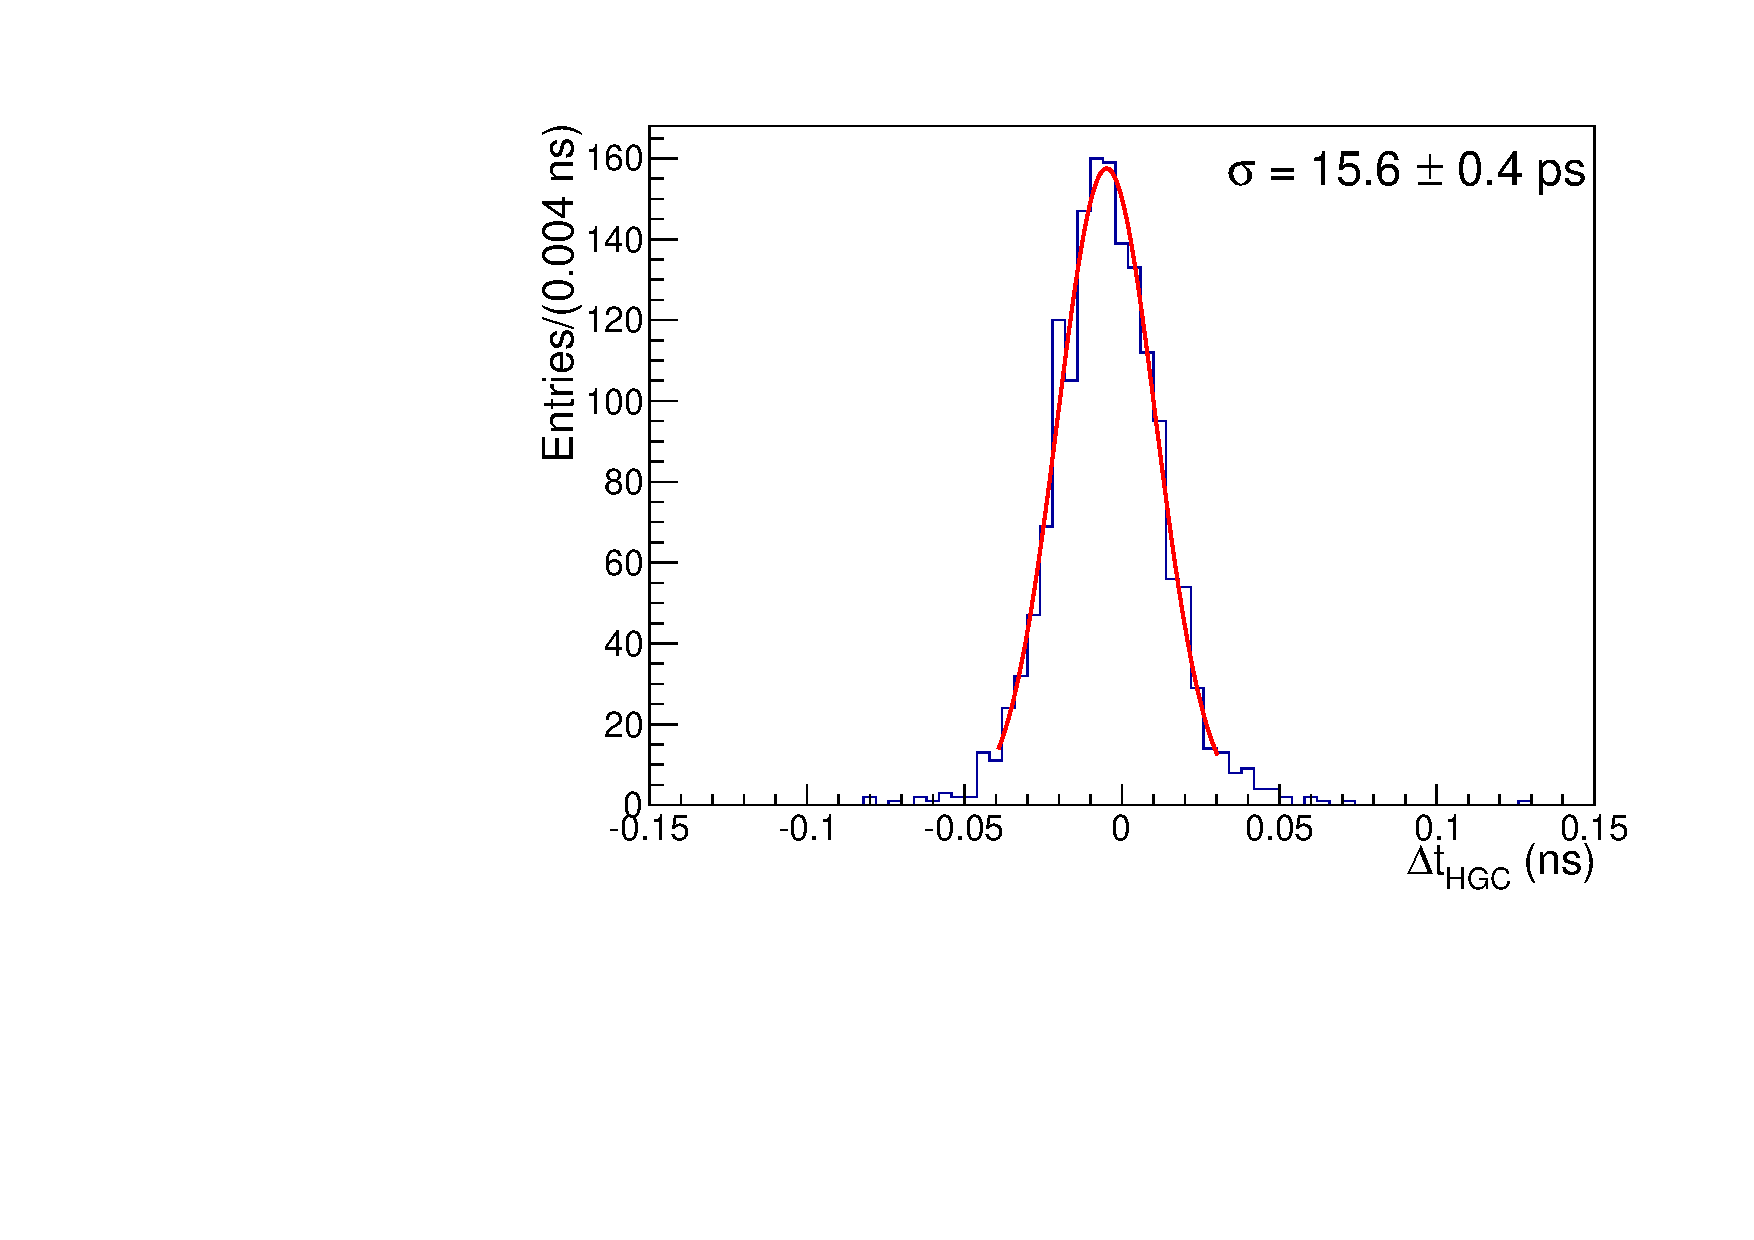
\includegraphics[width=.32\textwidth]{deltaTPicoSilEventCharge104.pdf}
	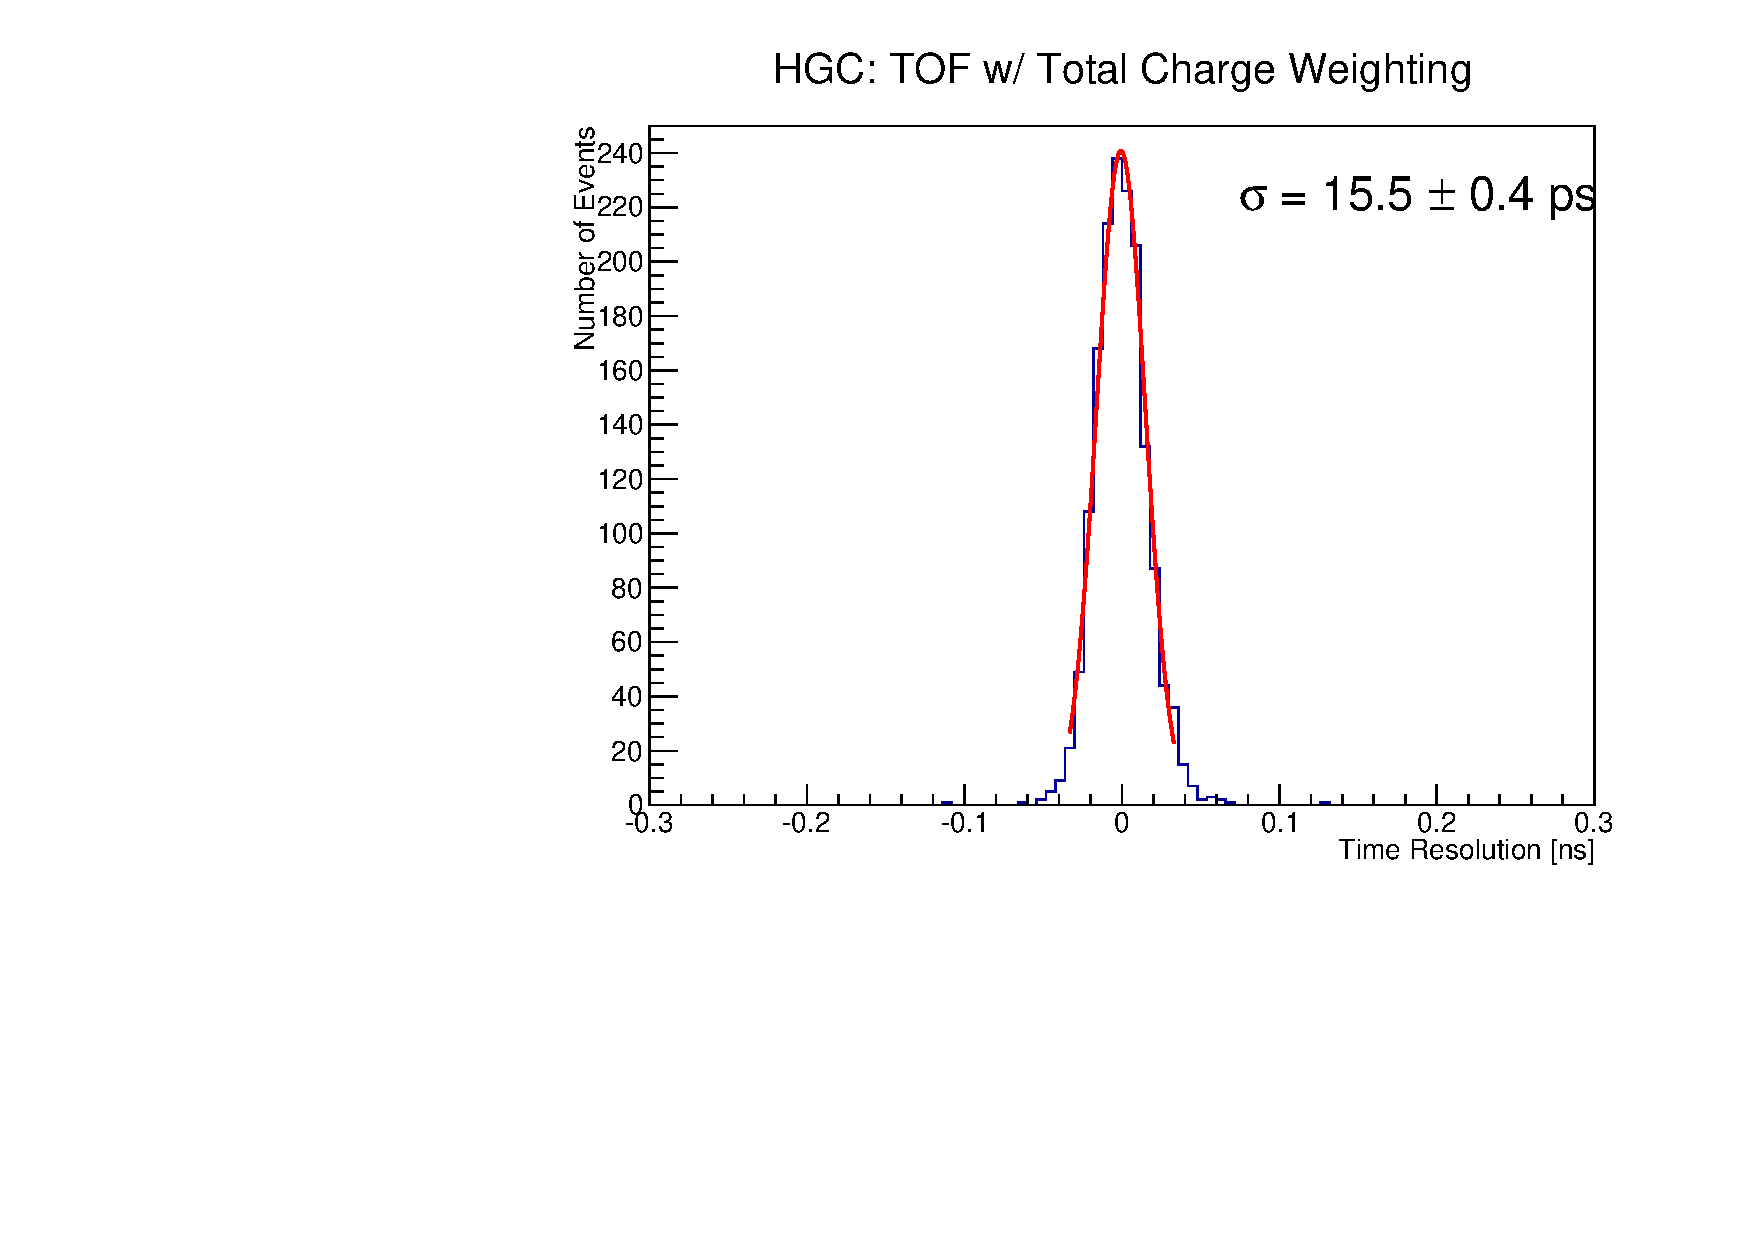
\includegraphics[width=.32\textwidth]{deltaTPicoSilTotalCharge104.pdf}
	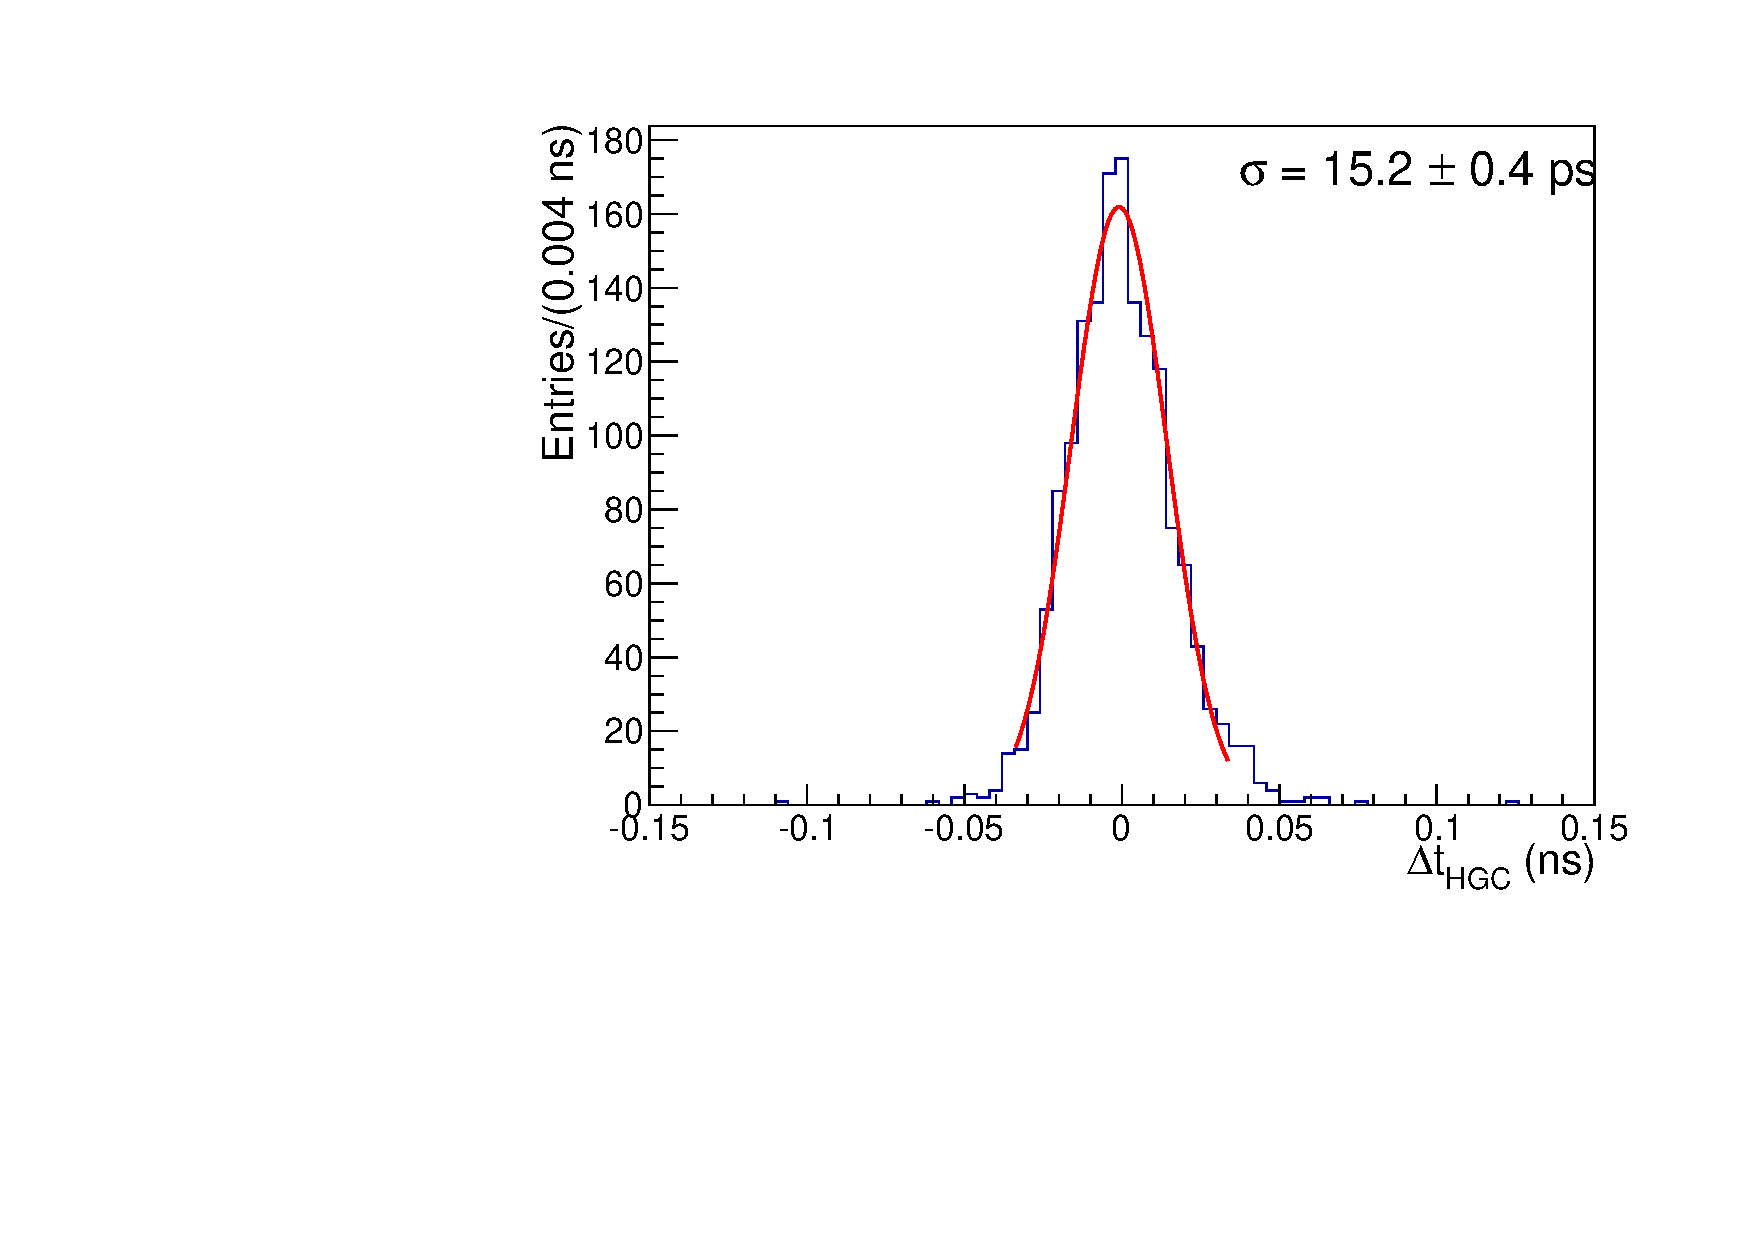
\includegraphics[width=.32\textwidth]{deltaTPicoSilLandauCharge104.pdf}
	\caption{TOF histograms of HGC pixels combined by event charge, total charge, and charge MPV.}
	\label{fig:HGC_event_total_MPV_104}
\end{figure*}

The above illustrates the transverse portion of this analysis. 
For the longitudinal aspect, the TOF values that are used to populate the HGC layer histograms in Figure \ref{fig:HGC_event_total_MPV_104} will be combined with the Photonis MCP-PMT TOF values for the right histogram in Figure \ref{fig:center_MCP_104}.
There are some relatively basic ways to combine the HGC layer with the Photonis.
The first method includes assigning an equal weighting to every pixel/detector that passes the cuts.
The second method includes equally weighting all HGC pixels that pass the cuts, then weighting the resultant TOF value equally with the Photonis TOF.
This second method can be written mathematically,
\[
\Delta t_i = \dfrac{ \Delta t_{MCP_i} }{2} + \dfrac{\sum\limits_{j=1}^N \Delta t_{HGC_{ij}} }{2\times N},
\]
\[
event\ i,\ \ N\ HGC\ pixels\ passing\ cuts.
\]
The results from these two methods can be seen in Figure \ref{fig:m12}. 
Note that these two methods are very elementary -- especially the first method, which weights the ring pixels too much, and the center pixel and Photonis too little -- but they are brought up now because one of them will be used later in another scenario. 
Here however, both methods (utilizing up to 8 detectors) gave a worse time resolution than just the central HGC pixel.

\begin{figure*}[!htbp]
\centering
	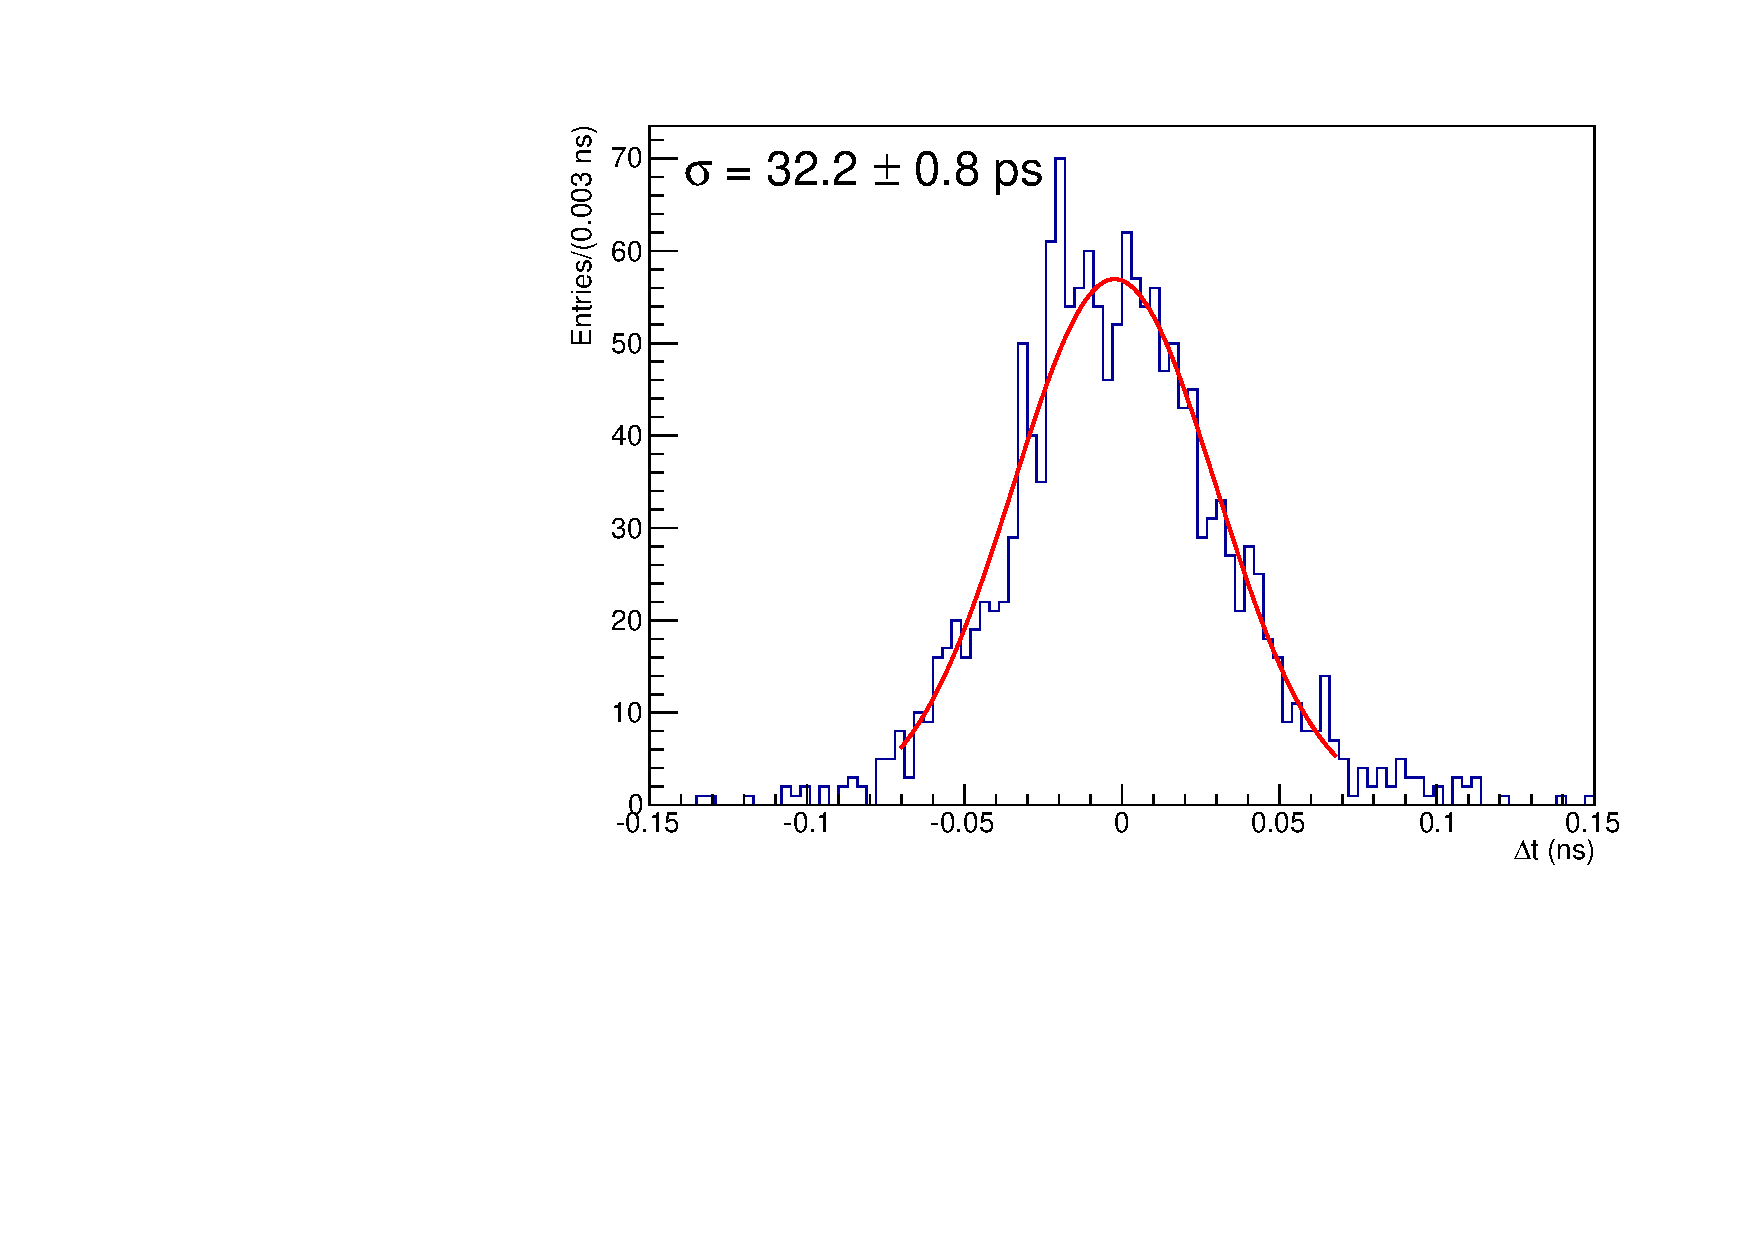
\includegraphics[width=.49\textwidth]{deltaT_PicoSil_MCP_Equal104.pdf}
	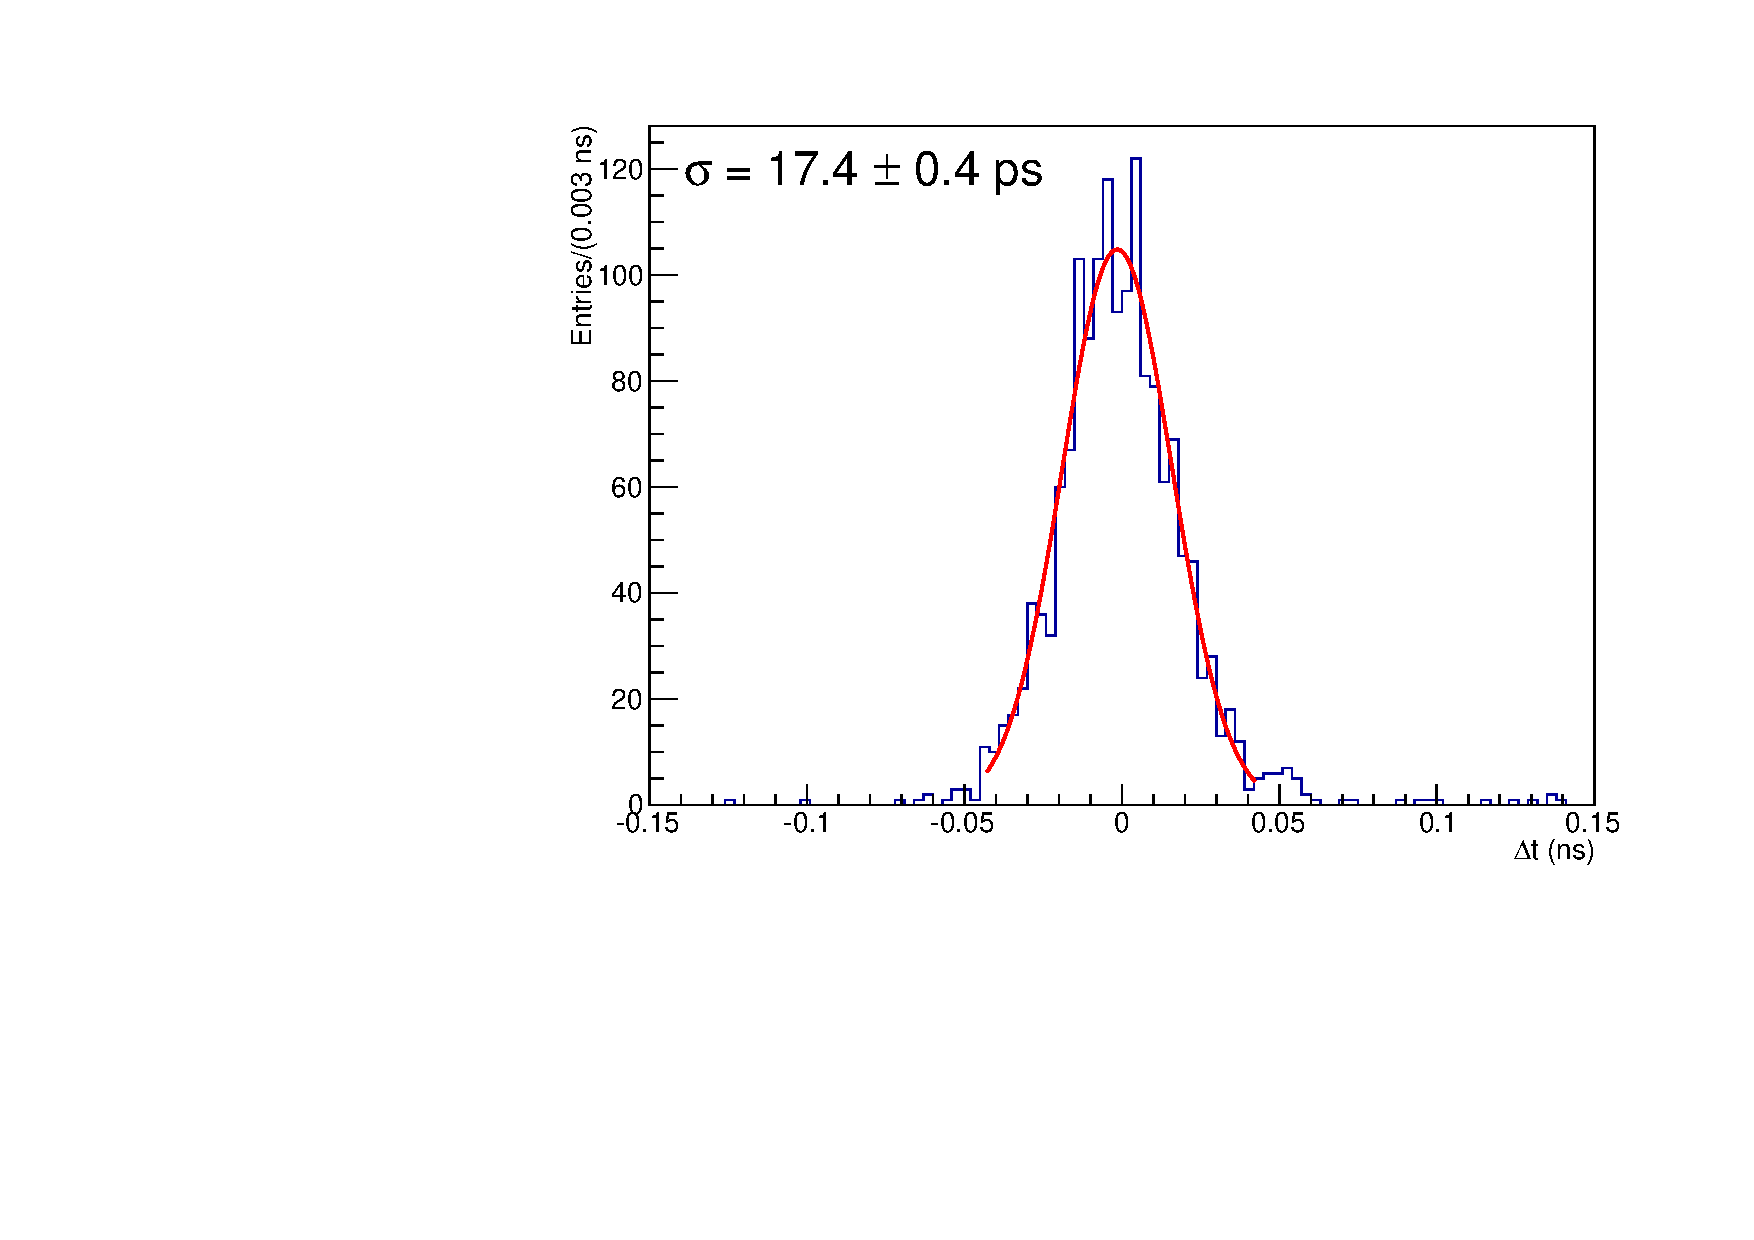
\includegraphics[width=.49\textwidth]{deltaT_PicoSilEqual_MCP_Equal104.pdf}
	\caption{Implementation of basic methods 1 (left) and 2 (right) as described in the text. }
	\label{fig:m12}
\end{figure*}

Smarter ways to combine the HGC layer with the Photonis MCP-PMT include combining every HGC pixel and the Photonis using the event charge and the total charge weighting methods described earlier.
Figure \ref{fig:HGC_MCP_event_total_104} gives the TOF histograms using these combination methods. 
While the total charge method shows an improvement in time resolution, the event charge method's time resolution of 14.2 ps is better than any HGC layer combination (Figure \ref{fig:HGC_event_total_MPV_104}) but worse than the resolution of just the Photonis (Figure \ref{fig:center_MCP_104}).

\begin{figure*}[!htbp]
	\centering
	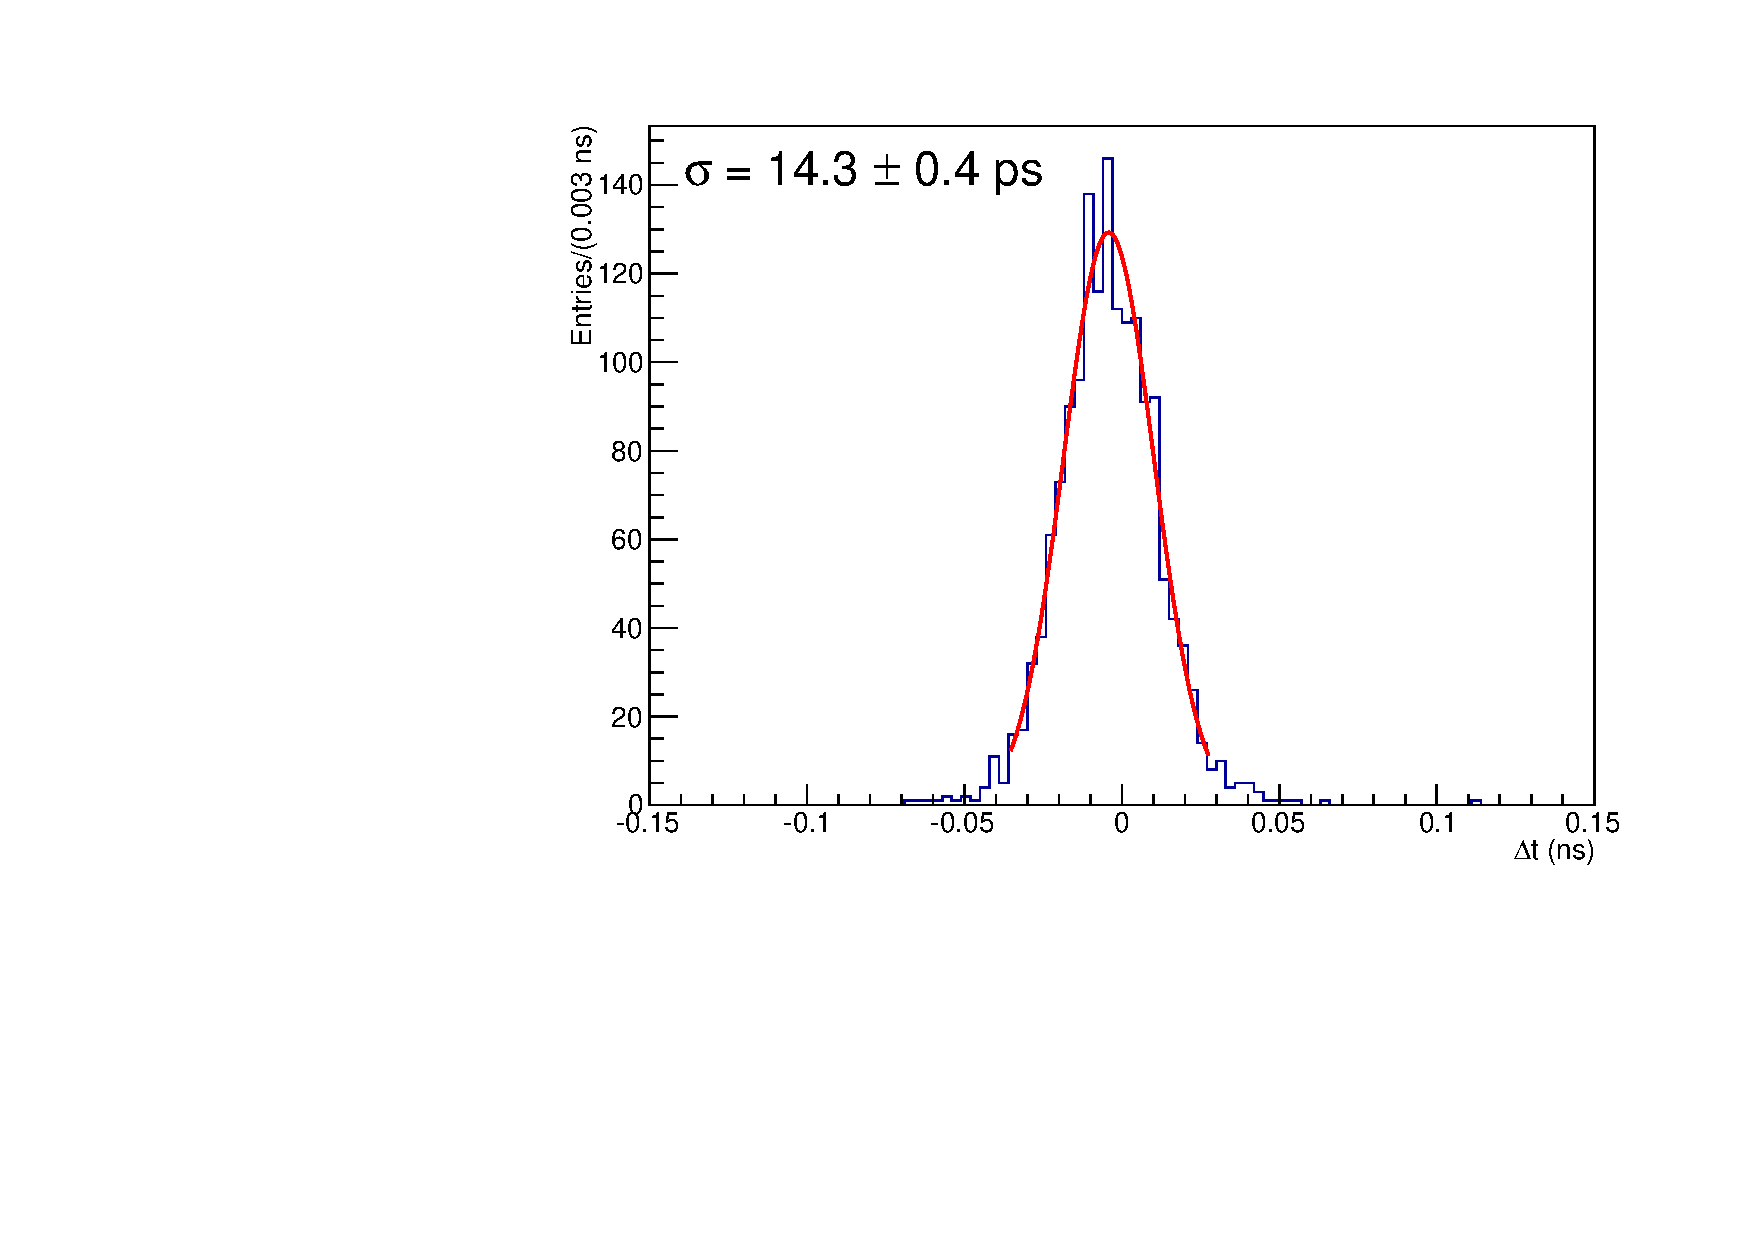
\includegraphics[width=.49\linewidth]{deltaT_PicoSil_MCP_EventCharge104.pdf}
	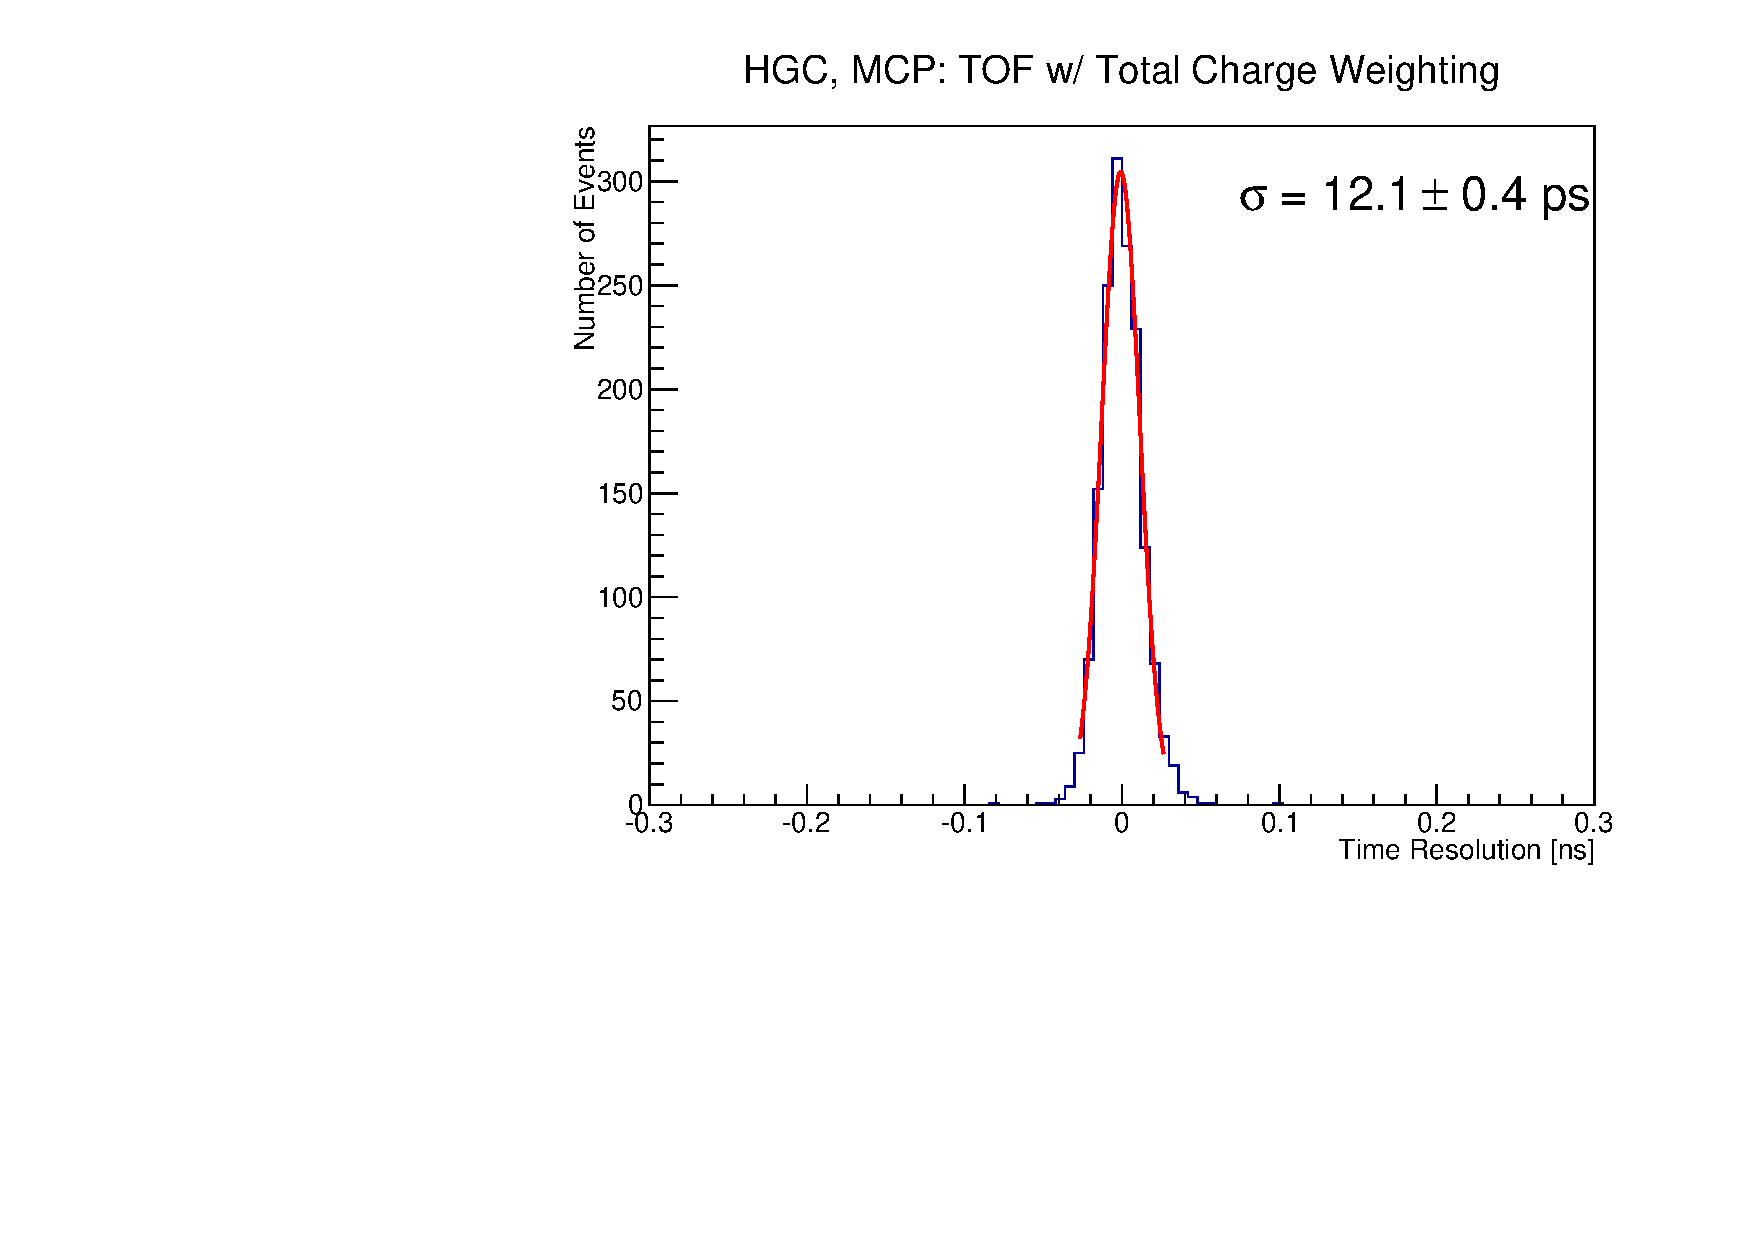
\includegraphics[width=.5\linewidth]{deltaT_PicoSil_MCP_TotalCharge104.pdf}
	\caption{TOF histograms of the HGC pixels and Photonis MCP-PMT, using event (left) and total (right) charge weightings.}
	\label{fig:HGC_MCP_event_total_104}
\end{figure*}

It turns out, however, that an HGC/Photonis combination using just charges is not the most accurate way to weight each detector. 
The first indication that there may be a smarter method comes from the equal weighting combination of the HGC center pixel (left Figure \ref{fig:center_MCP_104}; 15.9 ps) with the Photonis. 
Figure \ref{fig:CenterMCPEqual104} shows this combination. 
While the total charge-combined HGC layer has a better time resolution than the center pixel, the latter's equal combination with the Photonis is significantly better (11.4 ps compared to 12.1 ps). 
The equal weighting between devices is better than either of the charge weightings because it approximates that the same amount of charge flows into both detectors.
Even though the charges are not actually equal, this approximation is better than using the charge weighting \textit{because the relative gains of the HGC and Photonis is not known}. 
Put another way, a particle of a specific energy detected in the HGC would not return the same charge as a detection in the Photonis. 
Therefore, a better way to weight the TOF values would be to do either an event charge, total charge, or charge MPV weighting for the HGC pixel TOFs, then weight that value equally with the Photonis TOF (Figure \ref{fig:HGCMCP_event_total_MPV_104}). 
While the event charge weighting again gives the worst time resolution, the other two methods have a time resolution that is essentially the same as the HGC center pixel equally weighted with the Photonis MCP-PMT. 

\begin{figure}[!htbp]
	\centering
	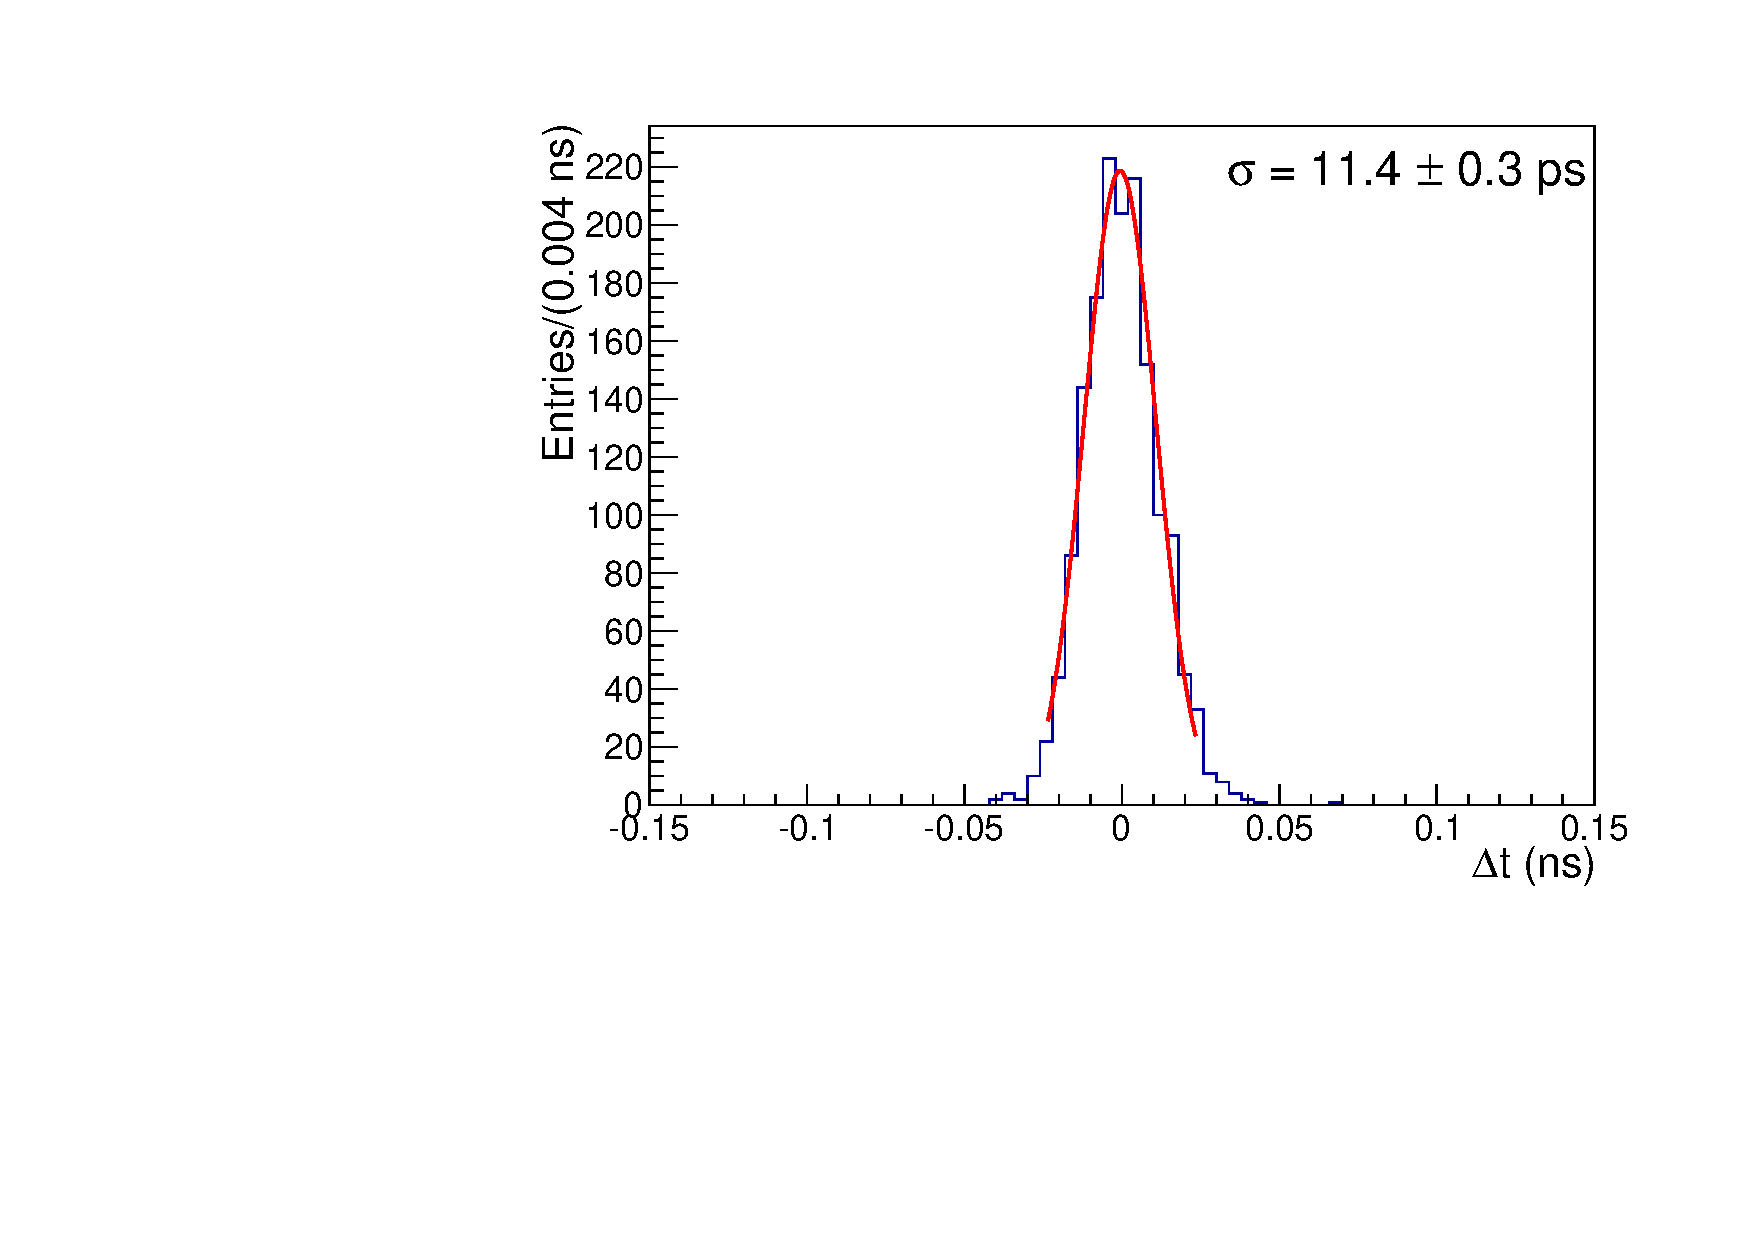
\includegraphics[width=\linewidth]{deltaT_Center_MCP_Equal104.pdf}
	\caption{TOF histogram weighting $\Delta t_{Center}$ and $\Delta t_{Photonis}$ by $\frac{1}{2}$.}
	\label{fig:CenterMCPEqual104}
\end{figure}


\begin{figure*}[!htbp]
	\centering
	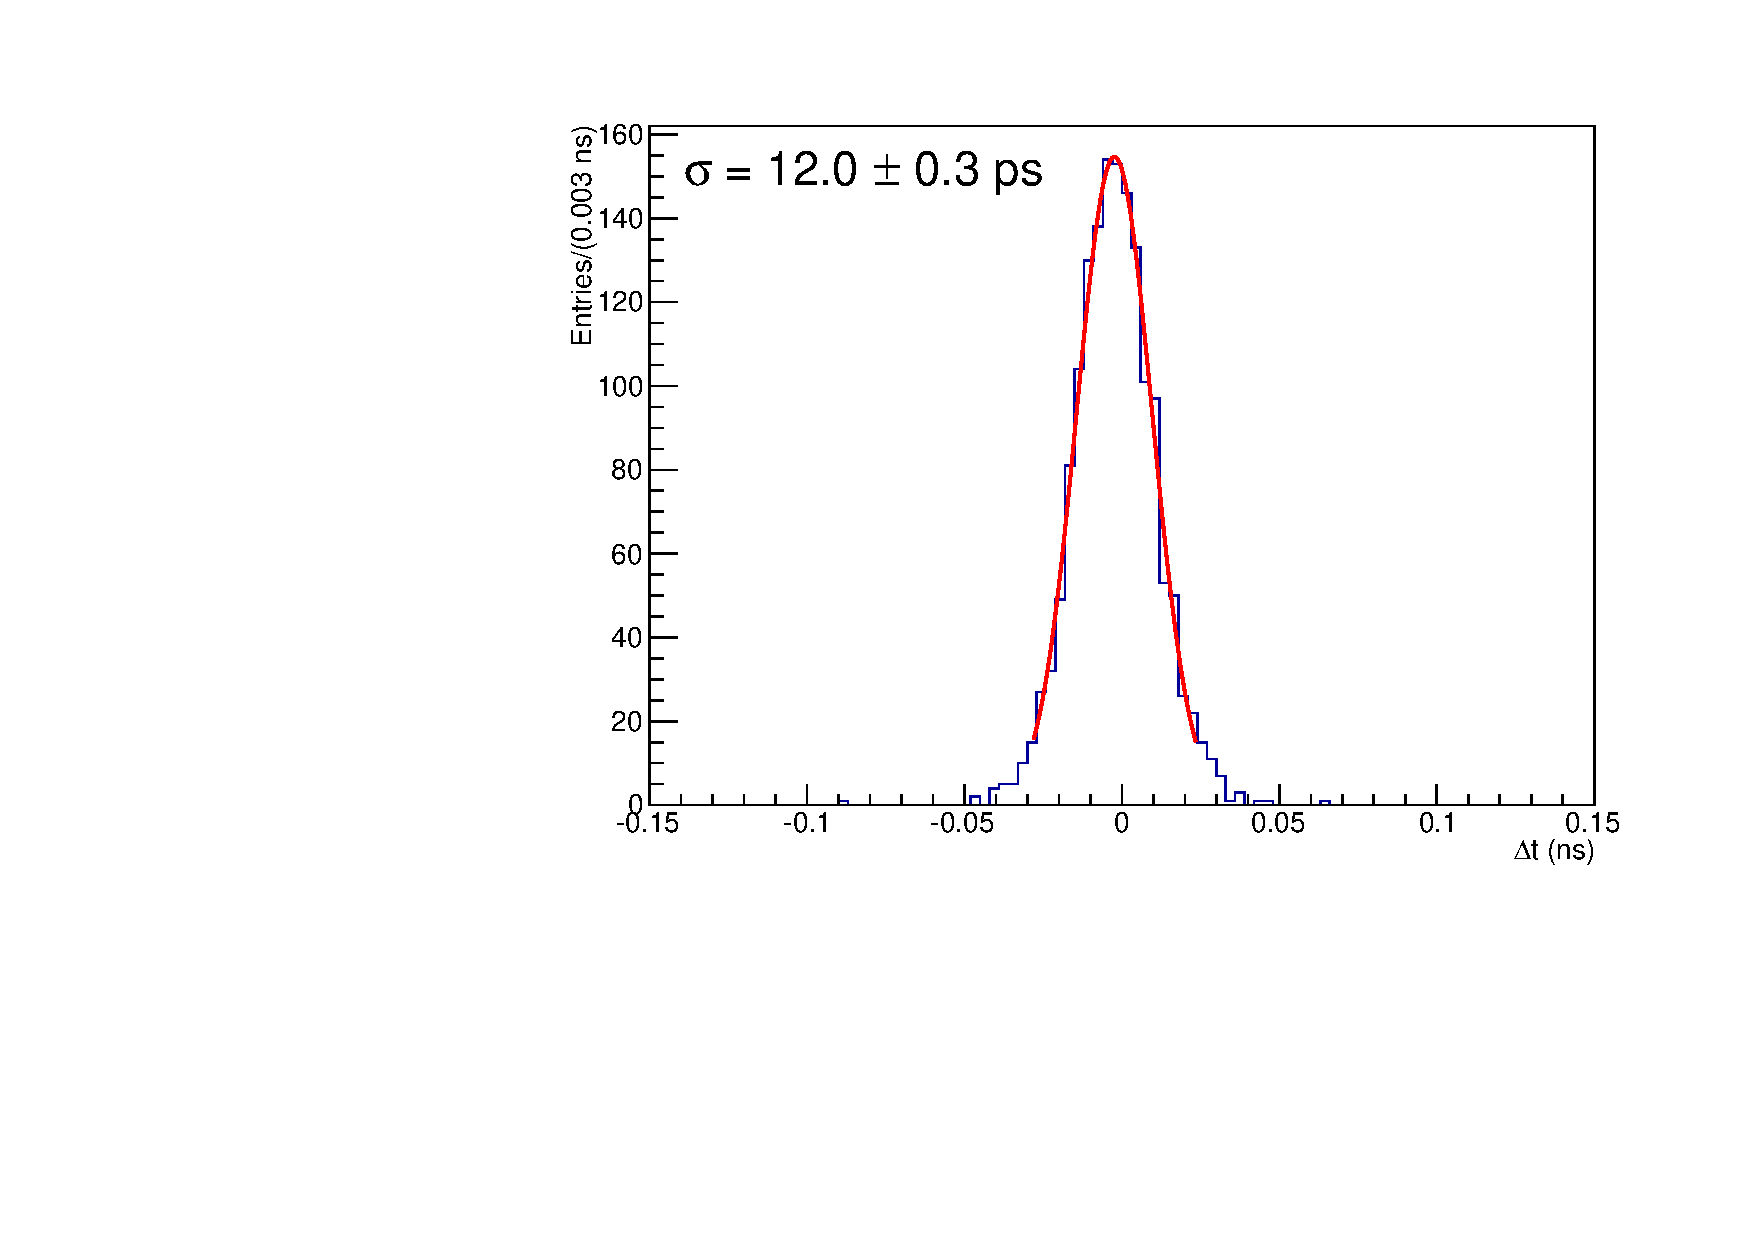
\includegraphics[width=.32\textwidth]{deltaT_PicoSilEventCharge_MCP_Equal104.pdf}
	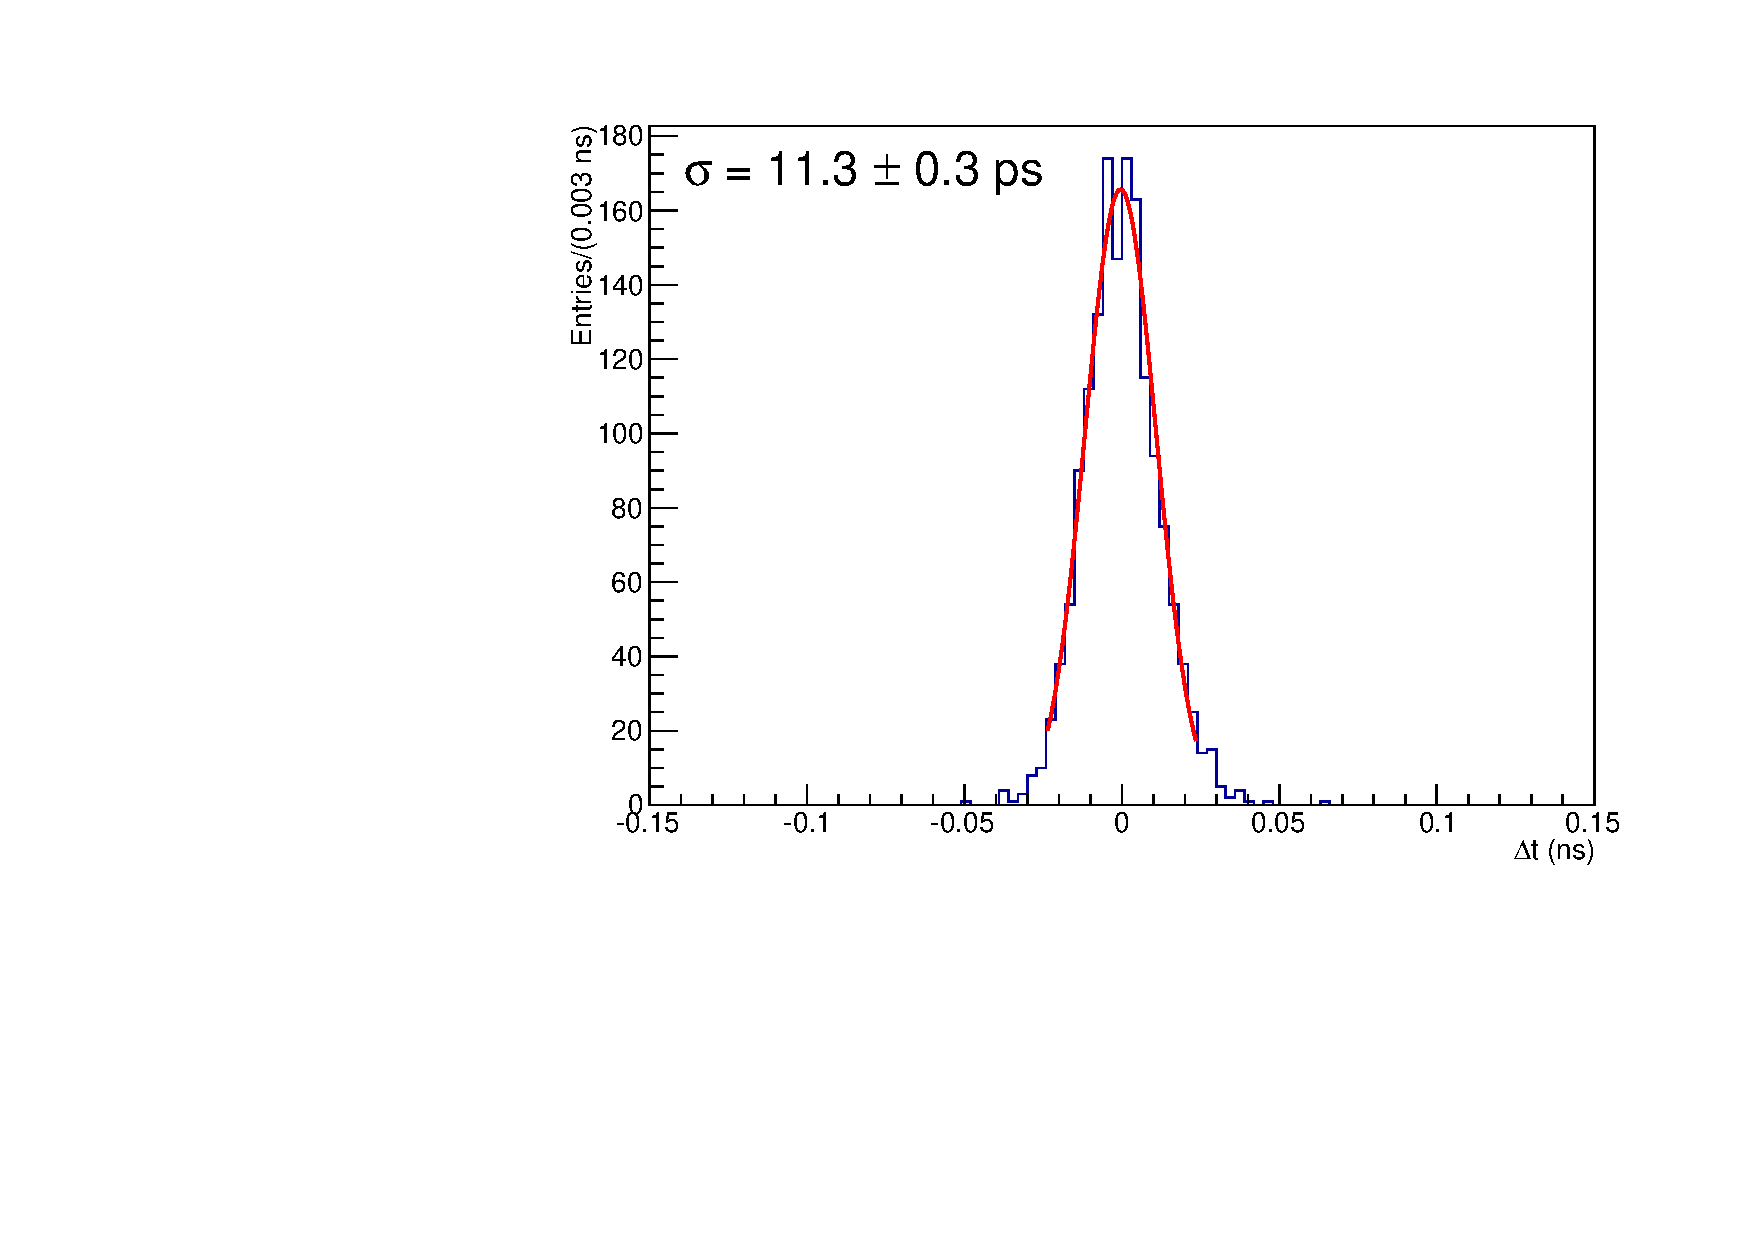
\includegraphics[width=.32\textwidth]{deltaT_PicoSilTotalCharge_MCP_Equal104.pdf}
	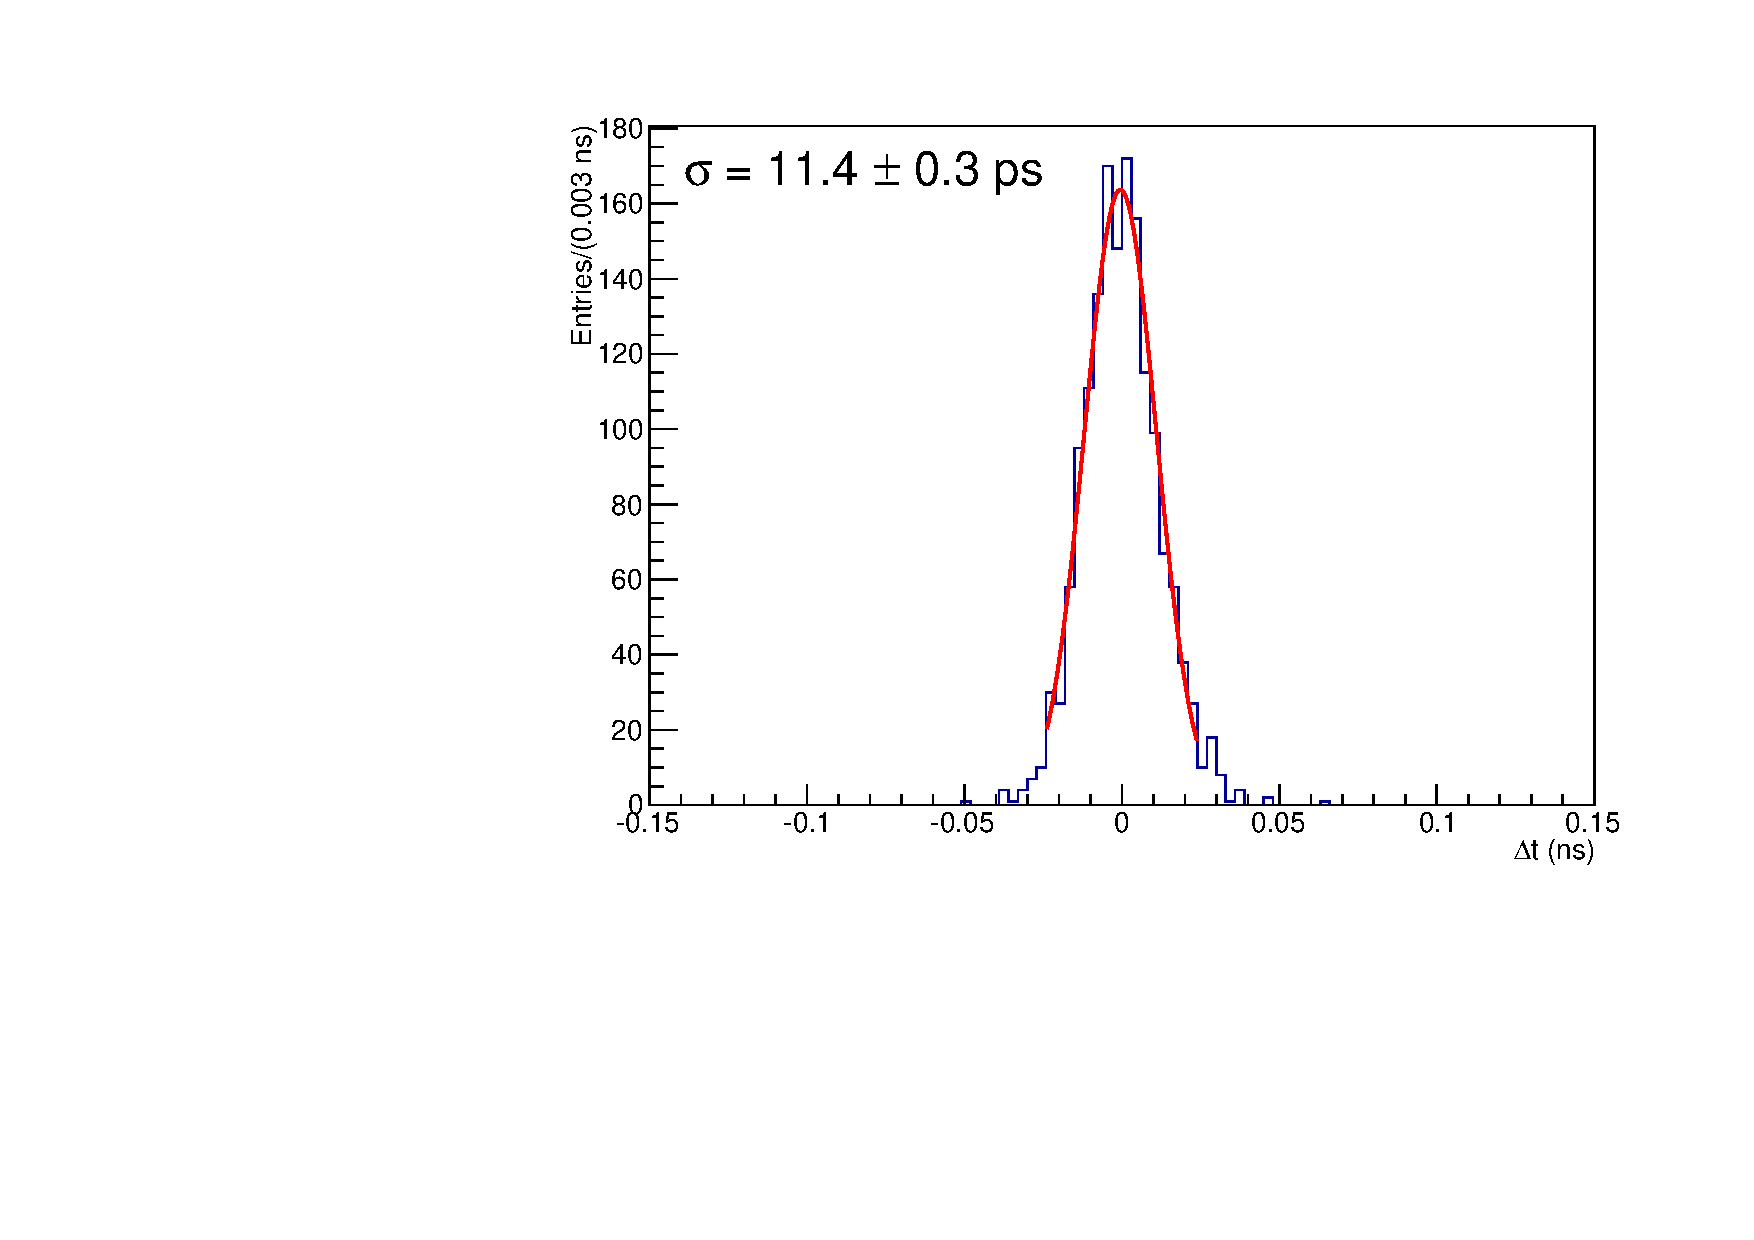
\includegraphics[width=.32\textwidth]{deltaT_PicoSilLandauCharge_MCP_Equal104.pdf}
	\caption{TOF histogram weighting $\Delta t_{HGC}$ and $\Delta t_{Photonis}$ by $\frac{1}{2}$, with $\Delta t_{HGC}$ computed via event (left), total (middle), and MPV (right) charge weightings.}
	\label{fig:HGCMCP_event_total_MPV_104}
\end{figure*}

This lack of improvement is most likely due to the relatively great time resolution of the central pixel compared to the ring pixels, which have a $\sigma$ that is around 4 times larger. 
Adding in the 6 ring pixels the time resolution only improved from $15.9 \pm 0.4$ ps to $15.5 \pm 0.4$ ps.
This improvement is small because the worse time resolutions of the outside pixels cannot contribute much to the already-good center pixel.
In this experiment, the test beam was focused onto the center pixel, which improves its time resolution compared to the other pixels. 
At the LHC, one pixel will not always be favored over the others in bunch crossings, and the most energetic part of the interaction may not interact with one of the pixels, so the pixel resolutions are expected to be similar.
While it does not seem useful in this experiment to add in the ring pixels, perhaps if they had a time resolution closer to the center pixel's, then adding them would lead to bigger improvements.
This statement is tested below.

Note that the time resolution values and their relative sizes given in the plots above are for this specific configuration.
Analyzing other runs will lead to changes in these values. 
The absorber thickness, distance, type, and the beam energy contribute to the varying values of $\sigma$.

\section{SKIROC2 Emulation}
For calorimetry at CMS, the SKIROC2 ASIC is a 64-channel front-end chip that reads out silicon PIN diodes.
Simply put, it reads out the pulse data from the detectors.
Compared to the DRS4 evaluation board, the SKIROC2 chip sacrifices accuracy for speed and cost-effectiveness.
Unfortunately, the chip has a digital jitter affecting the pulse time values, which places a lower bound on $\sigma$. 

\subsection{Background}
Previous studies have found that the jitter is described well by a Gaussian distribution of $\sigma=50$ ps, centered around 0.
Thus, if a detector consistently measured pulses at time $X$, then plotting all of these time values would be essentially a Dirac Delta function.
If these values were then read out by the SKIROC2 chip, then (for enough events) plotting these new values would give a Gaussian of $\sigma = 50$ ps, $\mu = X$.
However, as explained above, the initial time values are already Gaussian distributed, so reading the data out returns a convolution of the two Gaussian distributions. 
In other words, the new distribution will be a Gaussian of $\sigma > 50$ ps.

In order to simulate how multiple HGC layers with multiple pixels at the CMS experiment can improve the time resolution, each pixel's pulse time can be \textit{smeared} by 50 ps, according to a random sampling from a Gaussian distribution.
This new smeared time can then be used to calculate the TOF value by subtracting it from the Photek's pulse time, which is not smeared.
This process effectively simulates the SKIROC2 digitizer's jitter.

\begin{figure}[!htbp]
	\centering
	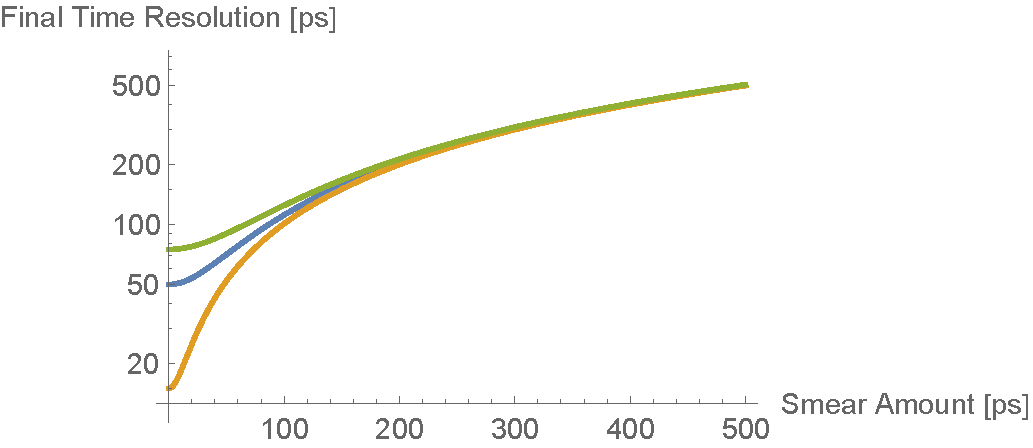
\includegraphics[width=\linewidth]{mathematica_plot.pdf}
	\caption{After being smeared by a large amount, detectors with different time resolutions (15 ps, 50 ps, 75 ps) approach the same value. Plotted in Wolfram Mathematica.}
	\label{fig:mathematica_plot}
\end{figure}

From Figure \ref{fig:mathematica_plot}, it can be observed that pixels with different initial $\sigma$ values will approach the same value when smeared by large amounts. 
This smearing can be used to test whether combining detectors of similar time resolution will be able to significantly improve the overall time resolution.

\subsection{50 ps Smear}
\subsubsection{Add Pixels Individually: All Pixels}
After smearing each pixel in the HGC layer by 50 ps, there are many ways to combine their TOF values. 
Before smearing, any form of equal weighting led to worse time resolutions, because the center pixel should be weighted more than the ring pixels.
However, as seen in Figure \ref{fig:mathematica_plot}, a 50 ps smear makes the time resolutions of the detectors closer. 
Yet, the ring pixels initially had time resolutions near 70-80 ps, so they still may not improve the time resolution as much as had the initial time resolutions been the exact same.

\begin{figure*}[!htbp]
\centering
	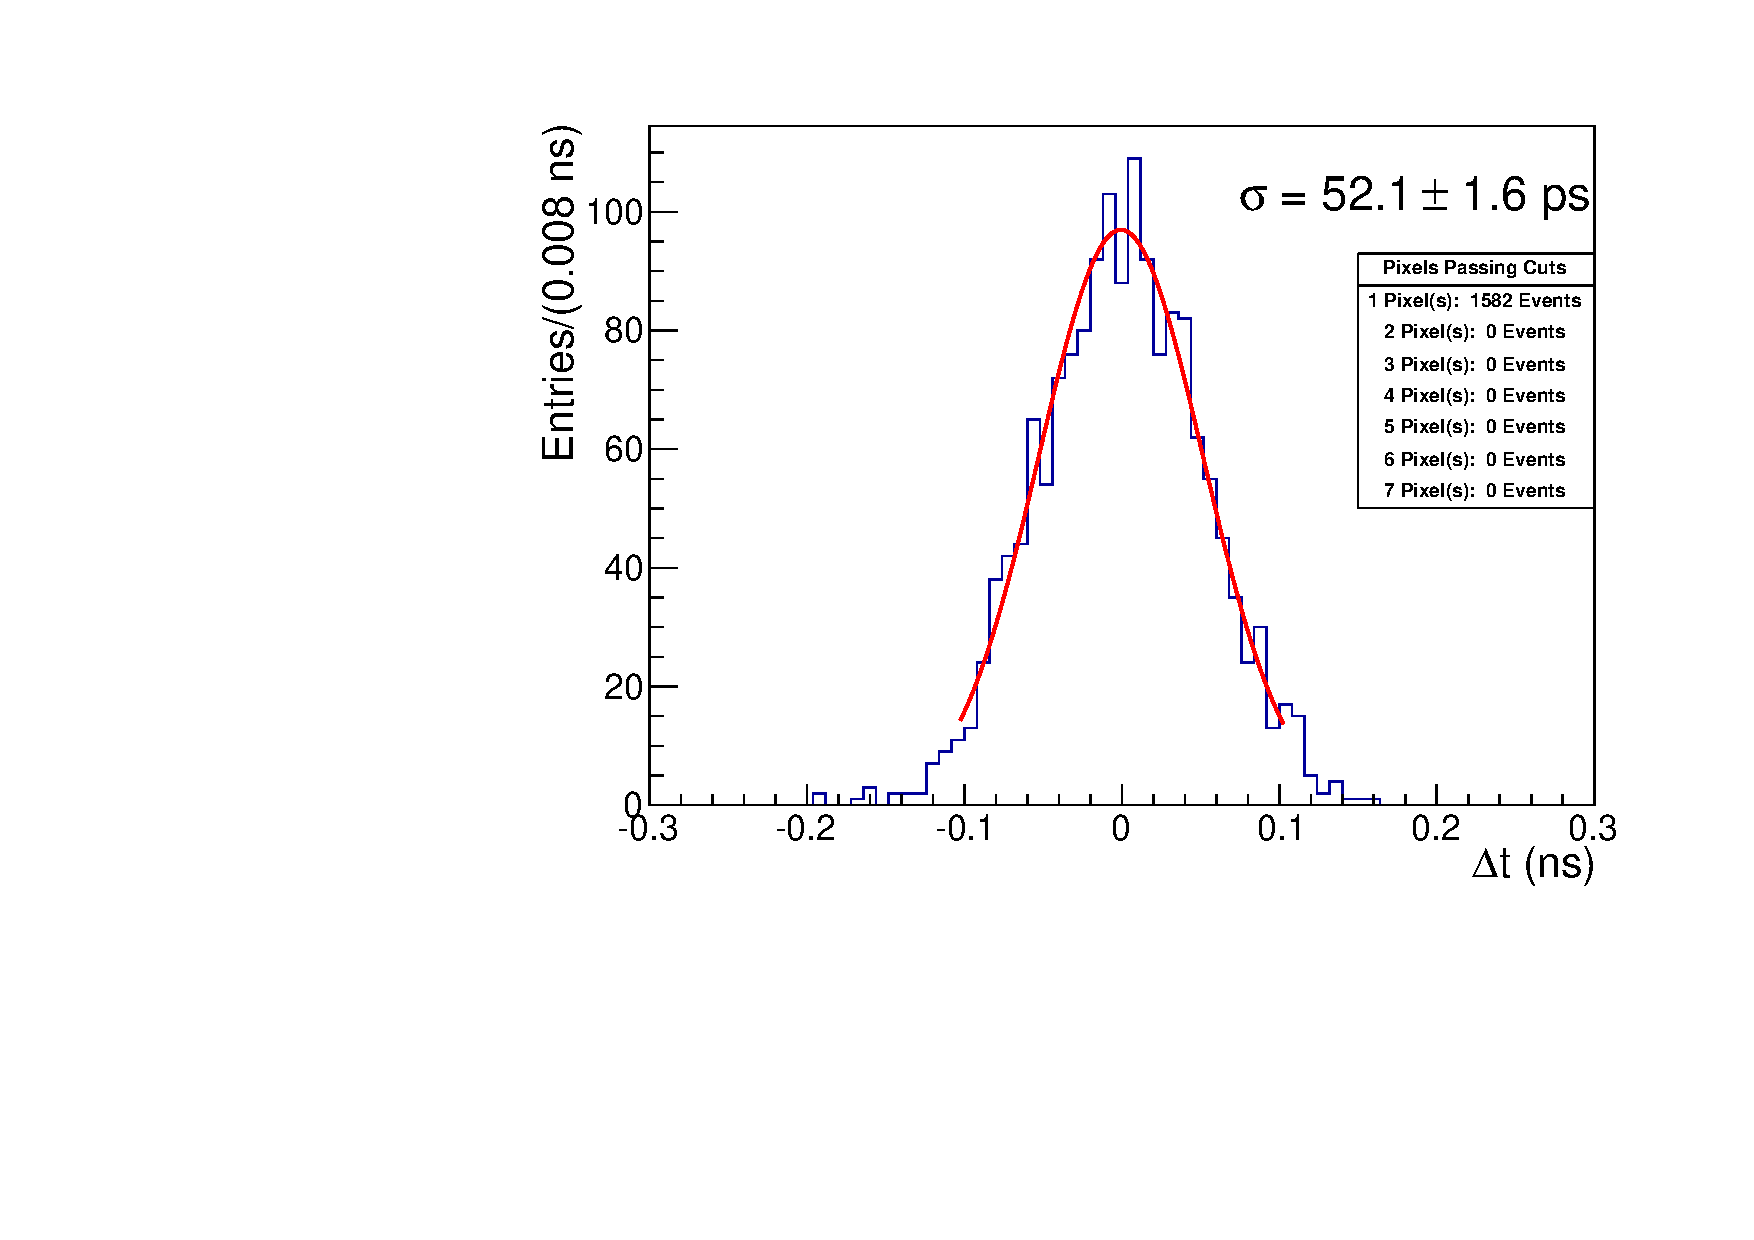
\includegraphics[width=0.35\textwidth]{SKIROC_1_Pixels50.pdf}
	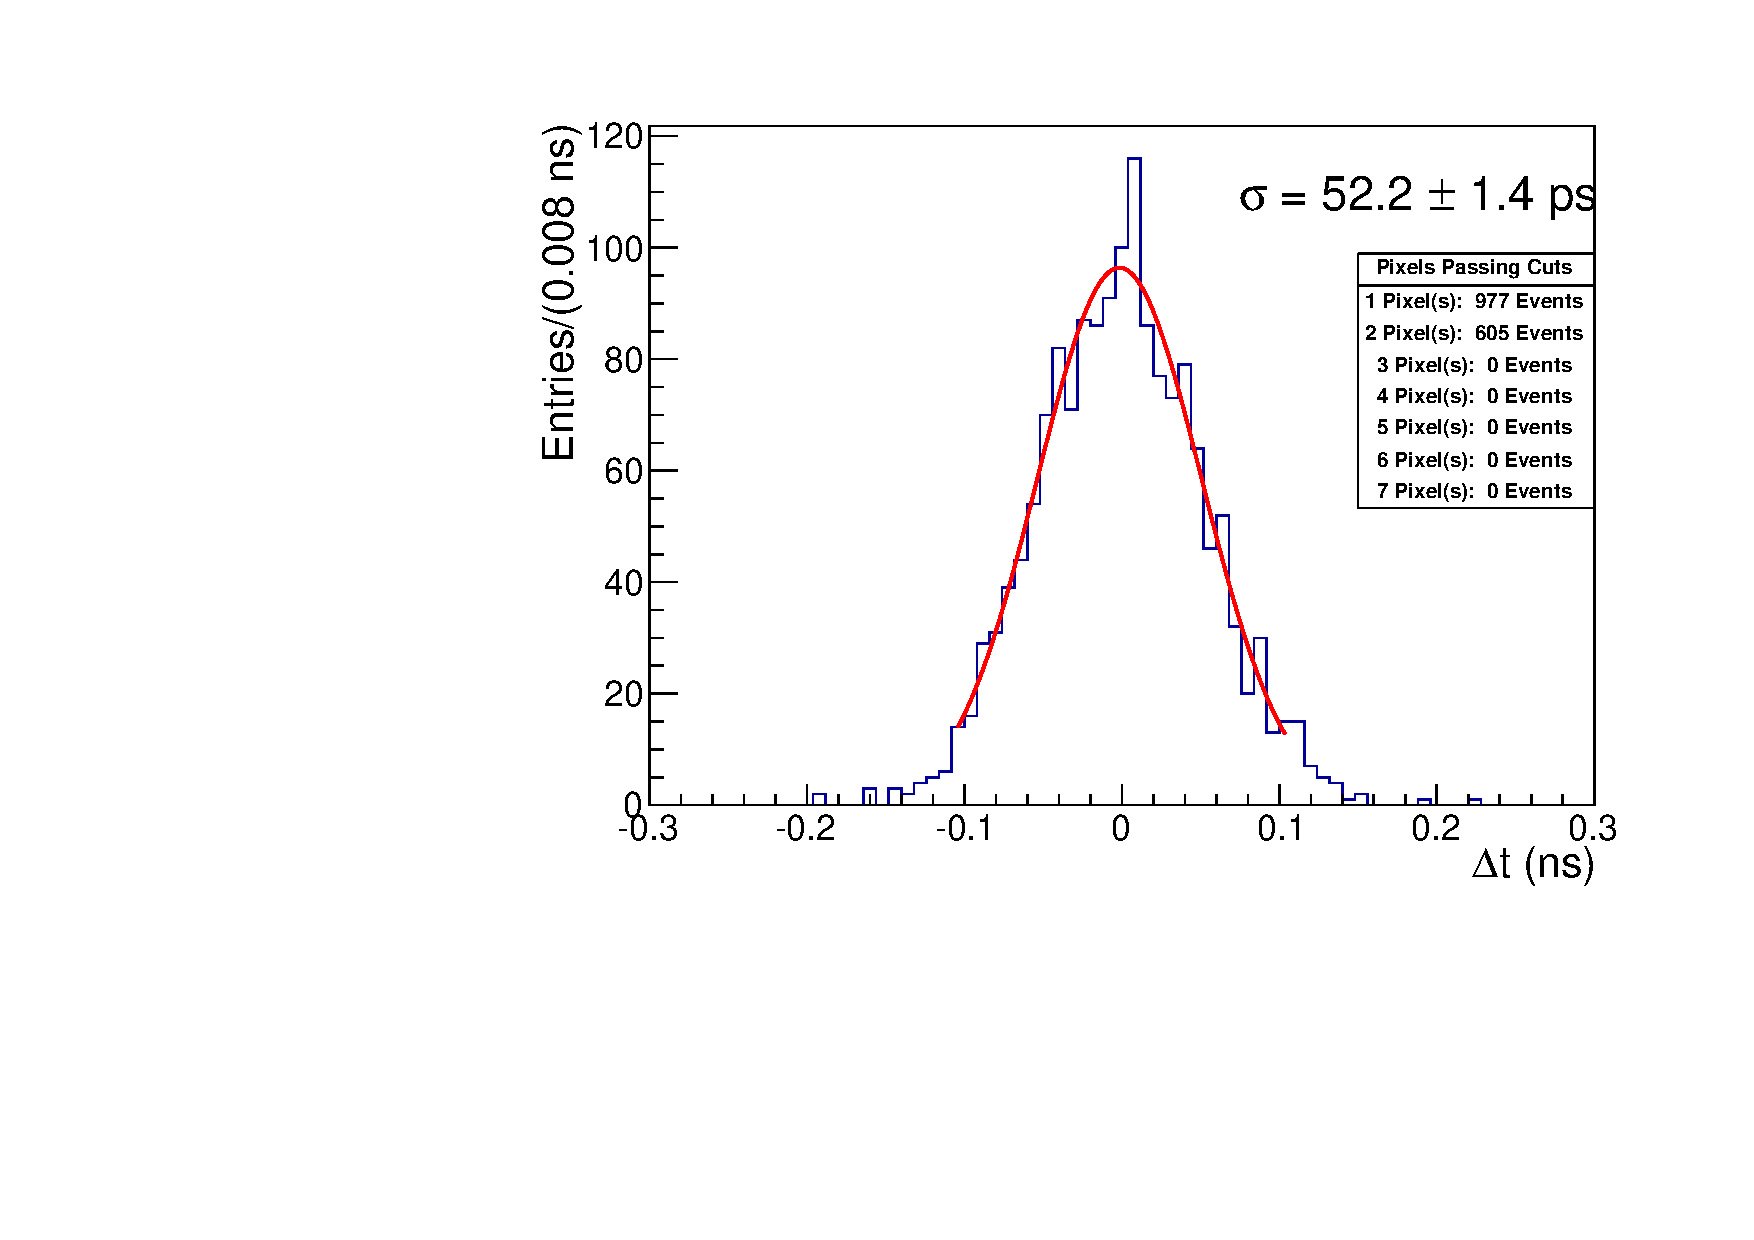
\includegraphics[width=0.35\textwidth]{SKIROC_2_Pixels50.pdf}
	
	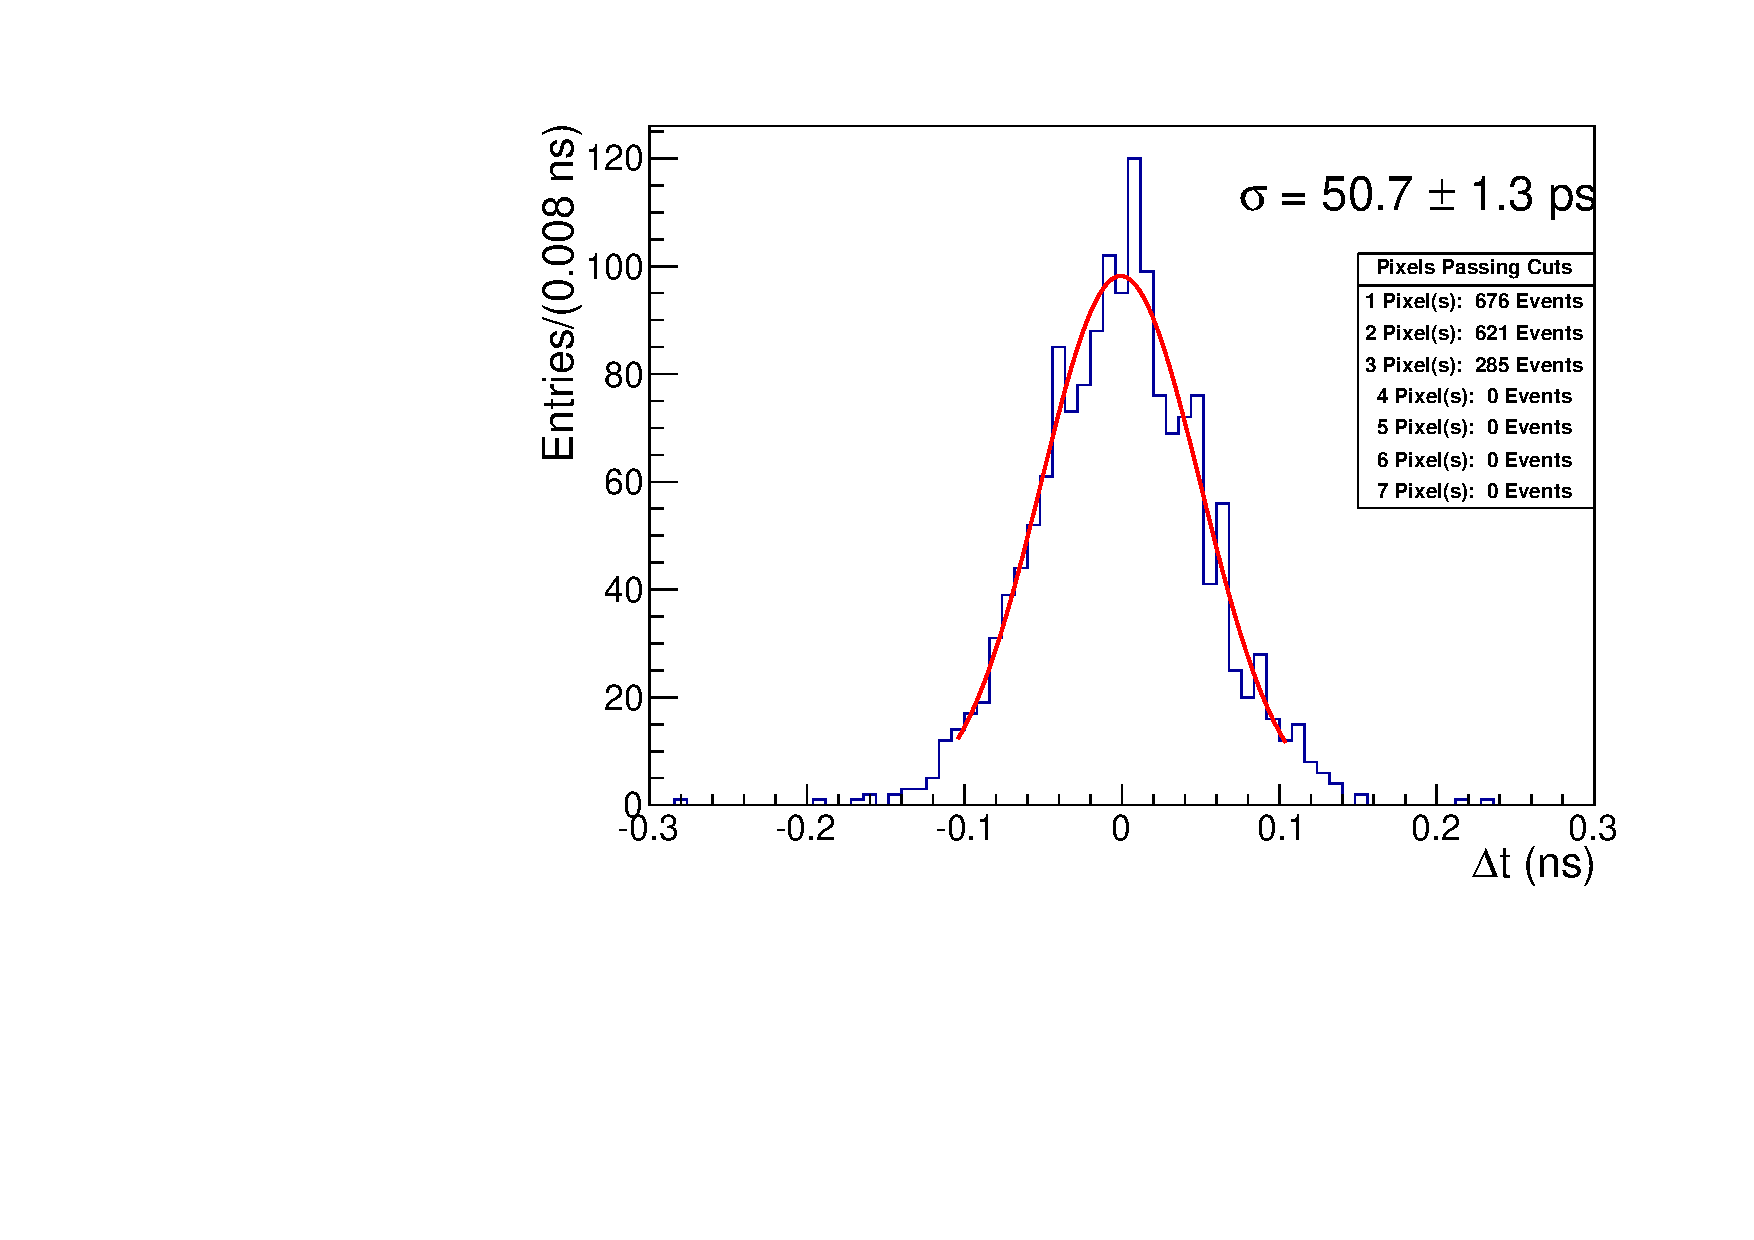
\includegraphics[width=0.32\textwidth]{SKIROC_3_Pixels50.pdf}
	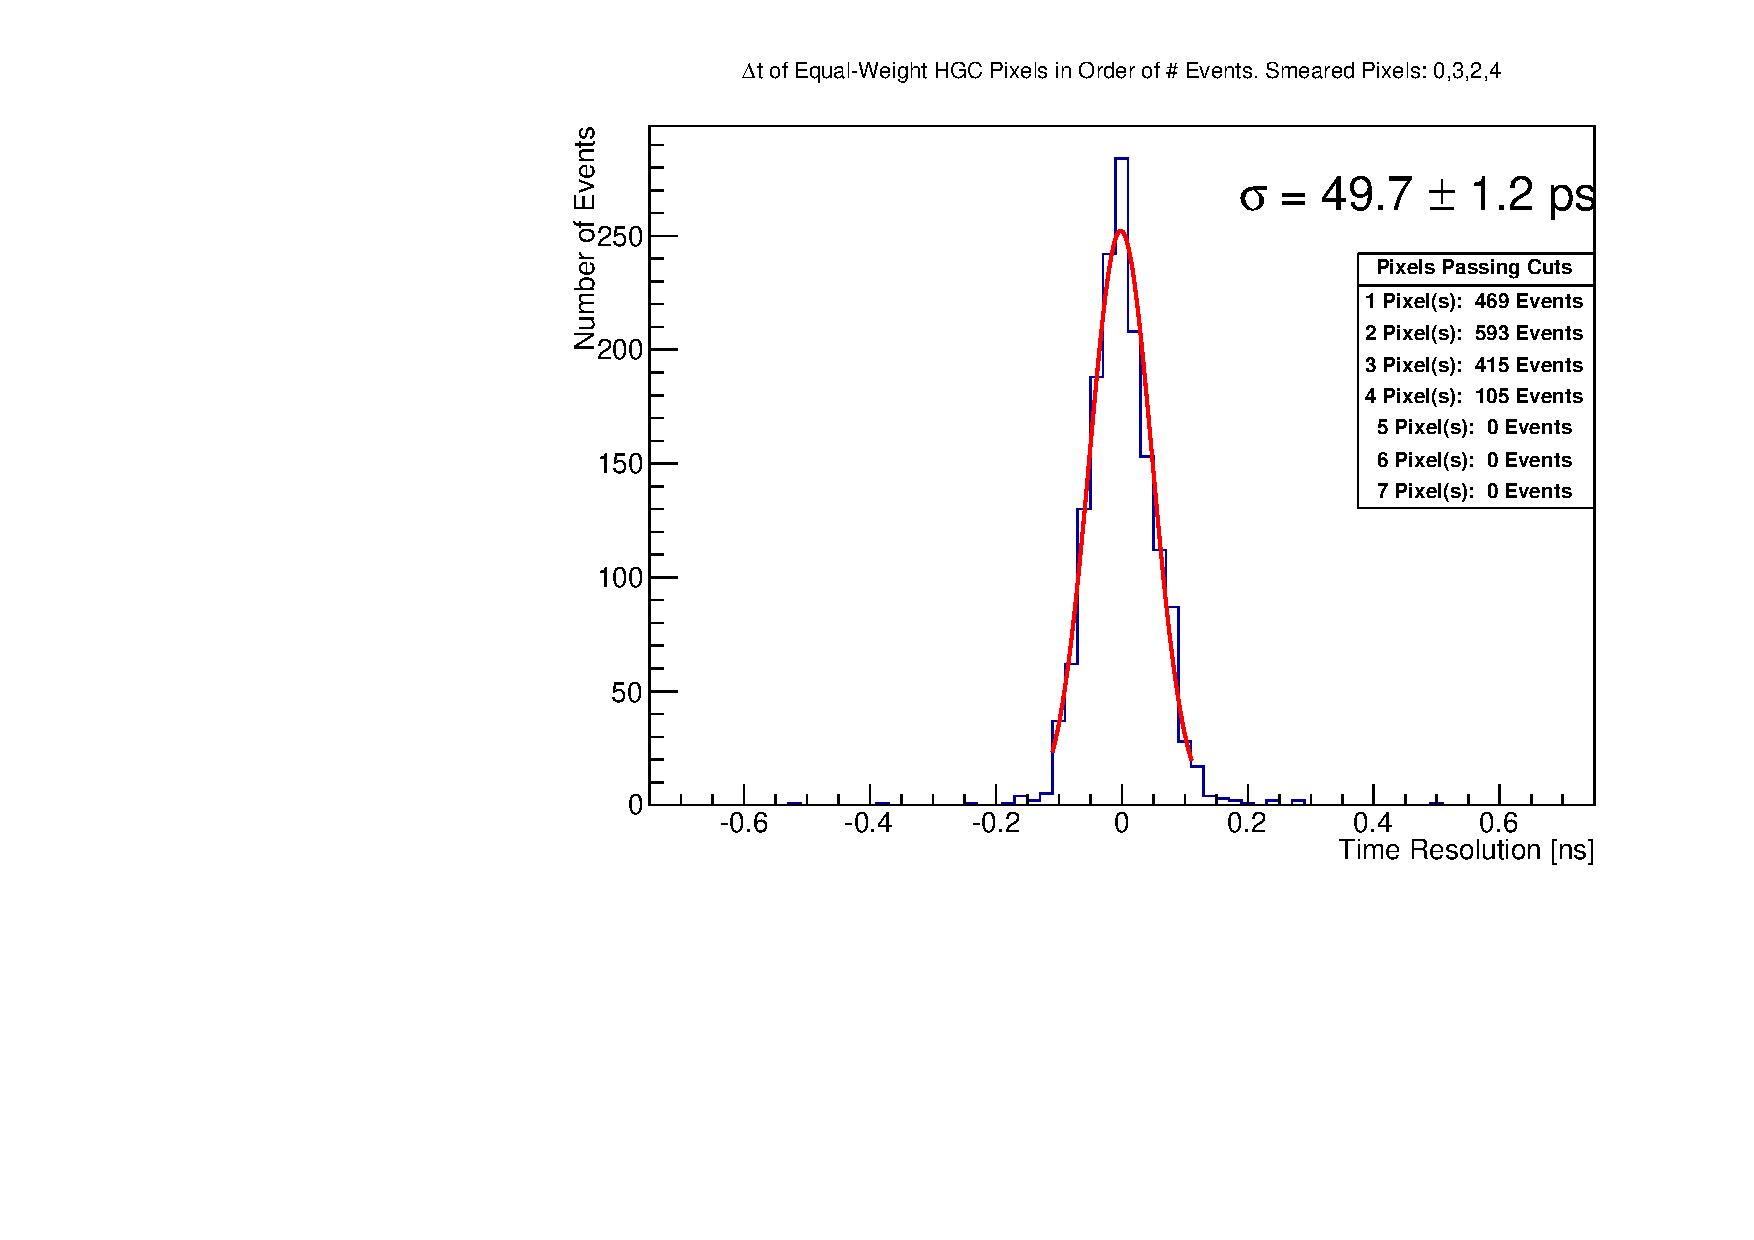
\includegraphics[width=0.32\textwidth]{SKIROC_4_Pixels50.pdf}
	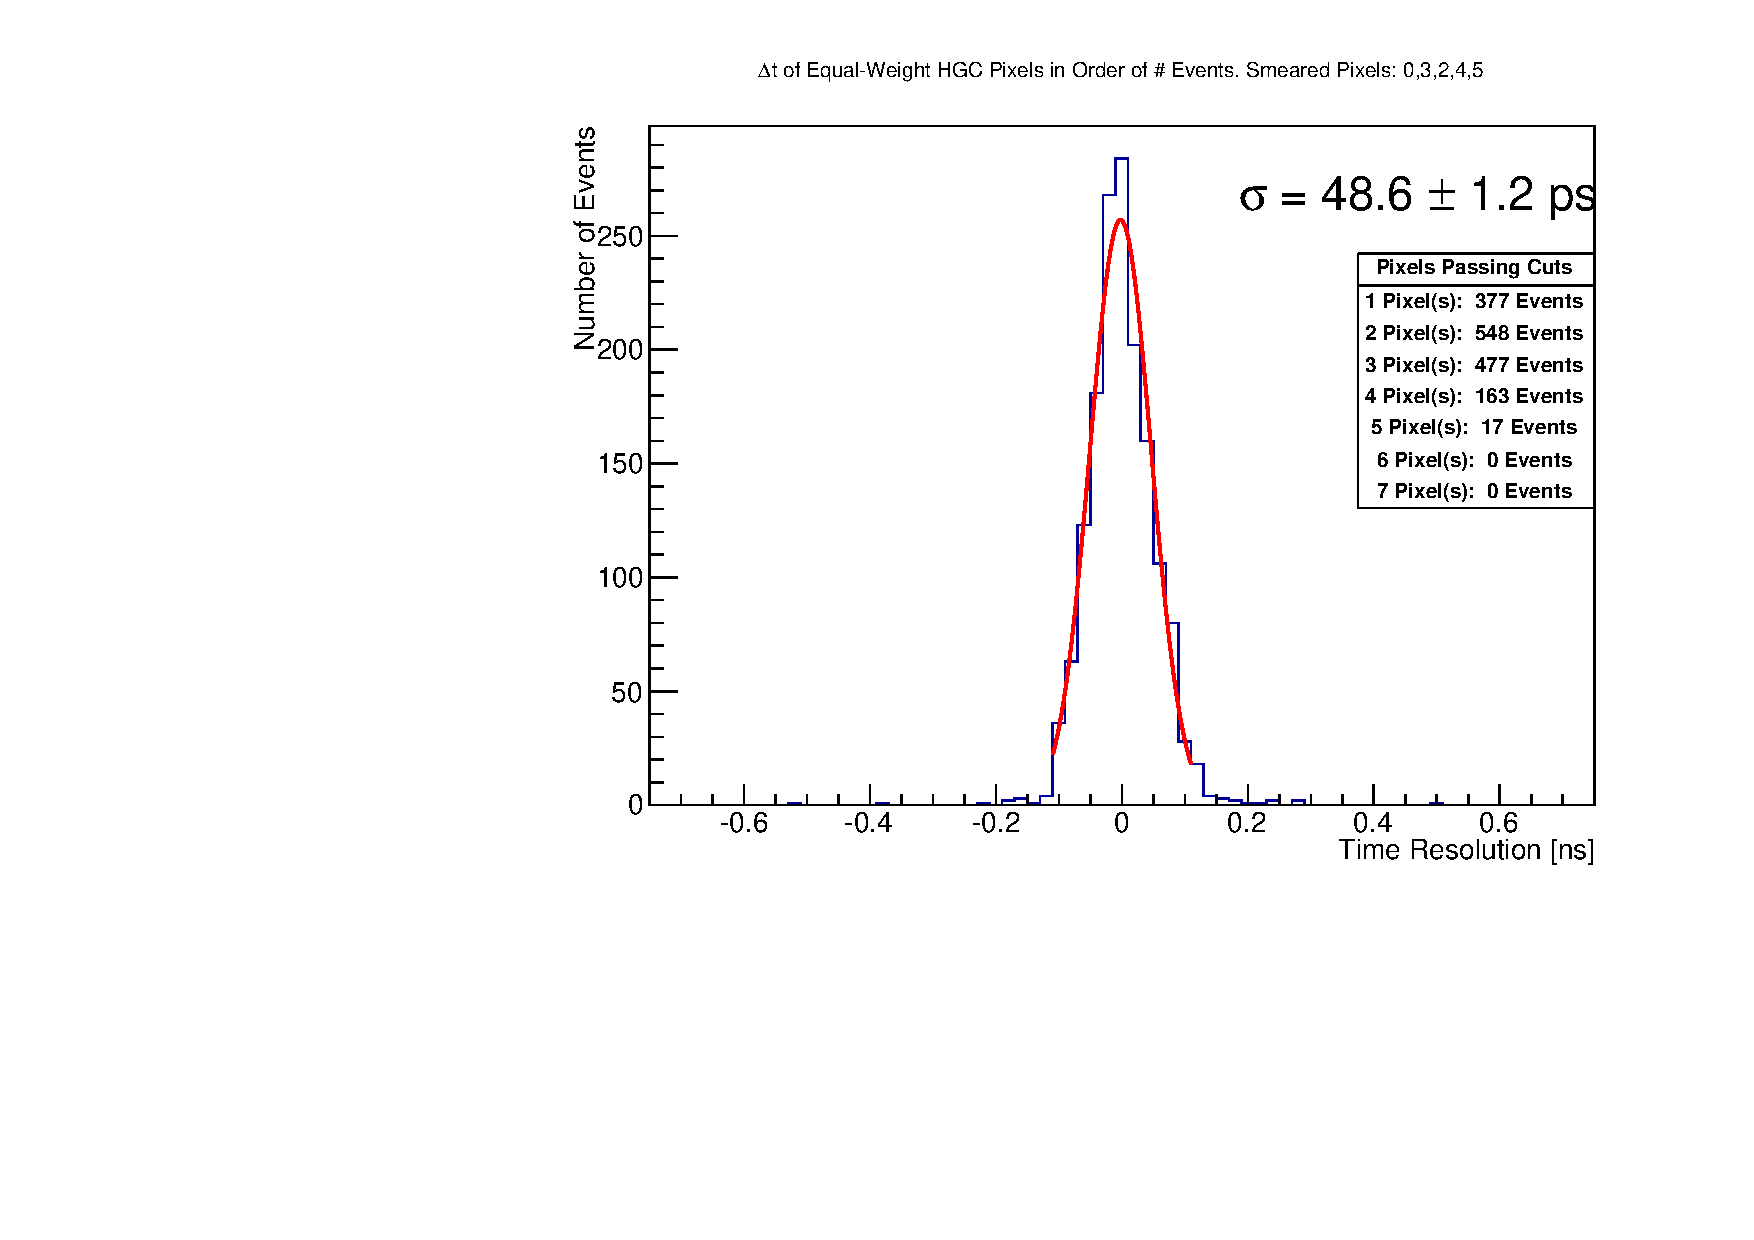
\includegraphics[width=0.32\textwidth]{SKIROC_5_Pixels50.pdf}
	
	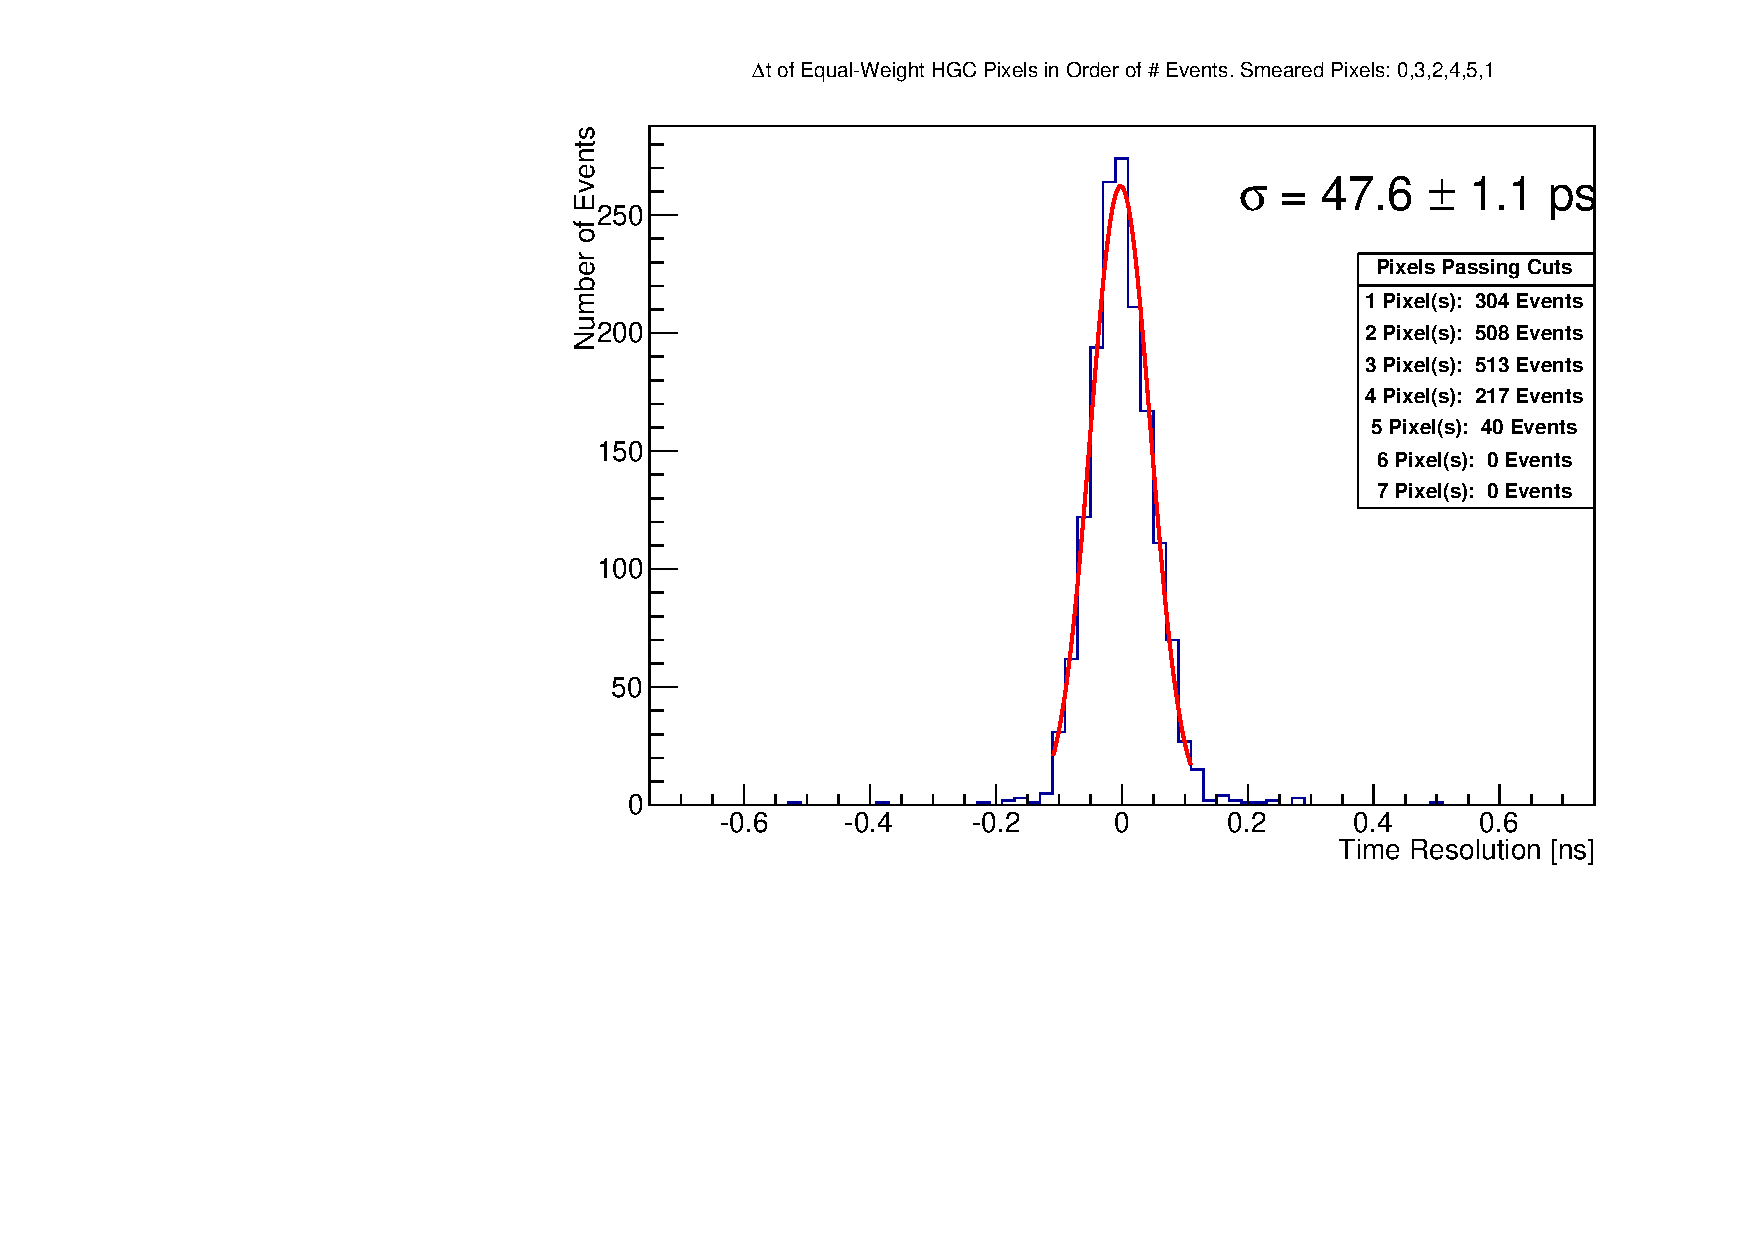
\includegraphics[width=0.35\textwidth]{SKIROC_6_Pixels50.pdf}
	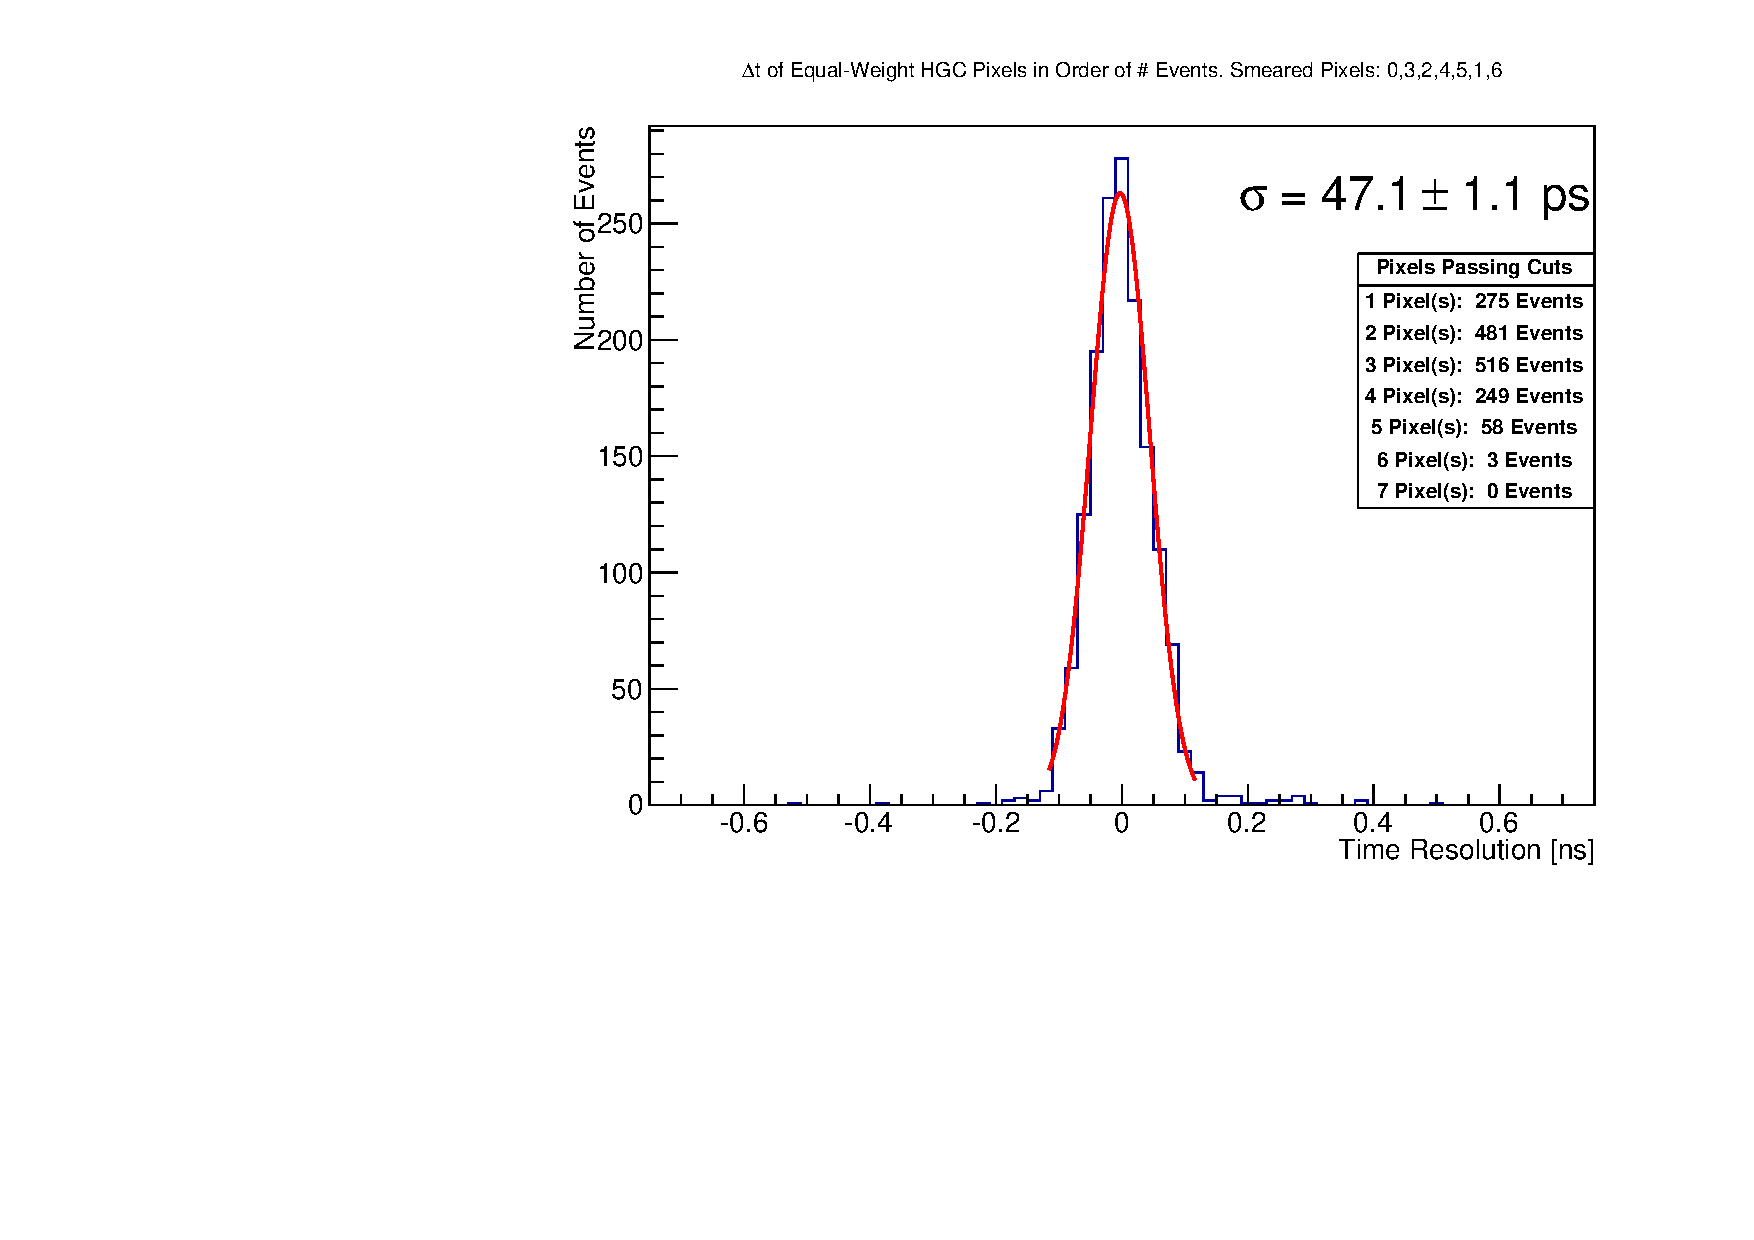
\includegraphics[width=0.35\textwidth]{SKIROC_7_Pixels50.pdf}
	\caption{Adding in pixels in decreasing events order.
		Each has been smeared by 50 ps.}
	\label{fig:50psAll}
\end{figure*}

In this case, it may also be useful to combine pixels with charge weighting, since the center pixel likely should still be weighted relatively heavier.
This will emphasize the lower time resolution of the center pixel.
However, equal weighting becomes a more valid method for larger smears, since the correlation between charge and a small $\sigma$ disappears.

Furthermore, it is interesting to observe how the time resolution improves with the addition of each pixel. 
This analysis can help determine the number of pixels to add before the time resolution improvement slows down.
Because only a handful of event cuts are passed by all 6 ring HGC pixels and the center pixel, adding pixels should not reduce the events.
In order to maintain a high event number, when two pixels are added together, the union of the events they pass -- instead of the intersection -- shall be the new number of events.
The intersection of passed events shall be the combined TOFs, and the remaining events shall simply use the individual TOF.

Each additional pixel shall be combined in decreasing order of number of events passed.
This strategy is implemented because pixels that pass more event cuts have a larger ability to influence the time resolution.
Figure \ref{fig:50psAll} shows the addition of each smeared pixel using an equal weighting method. 

\begin{figure*}[!htbp]
\centering
\begin{minipage}[t]{.49\textwidth}
	\centering
	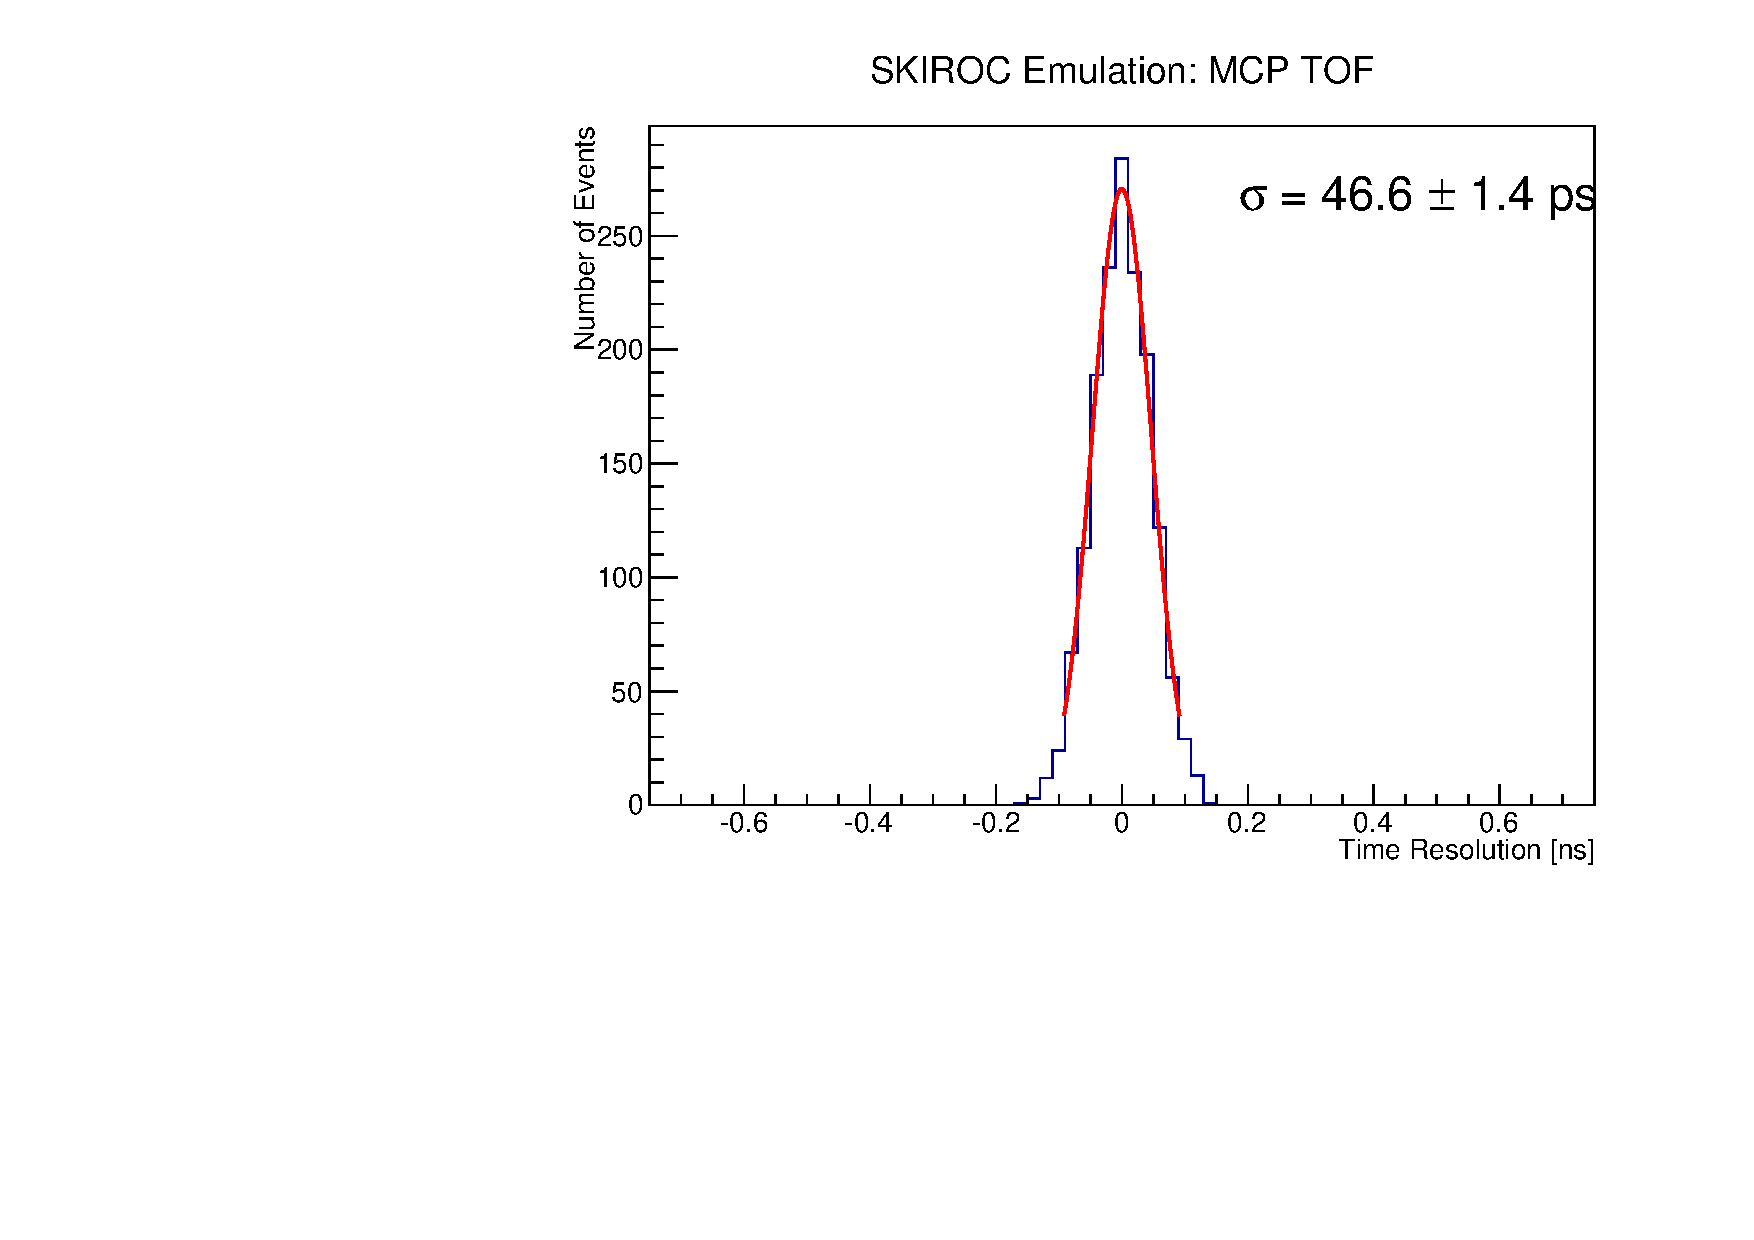
\includegraphics[width=\linewidth]{deltaTMCPSmear50.pdf}
	\caption{TOF histogram for 45ps smeared Photonis.}
	\label{fig:50p_MCP}
\end{minipage}\hfill
\begin{minipage}[t]{.49\textwidth}
	\centering
	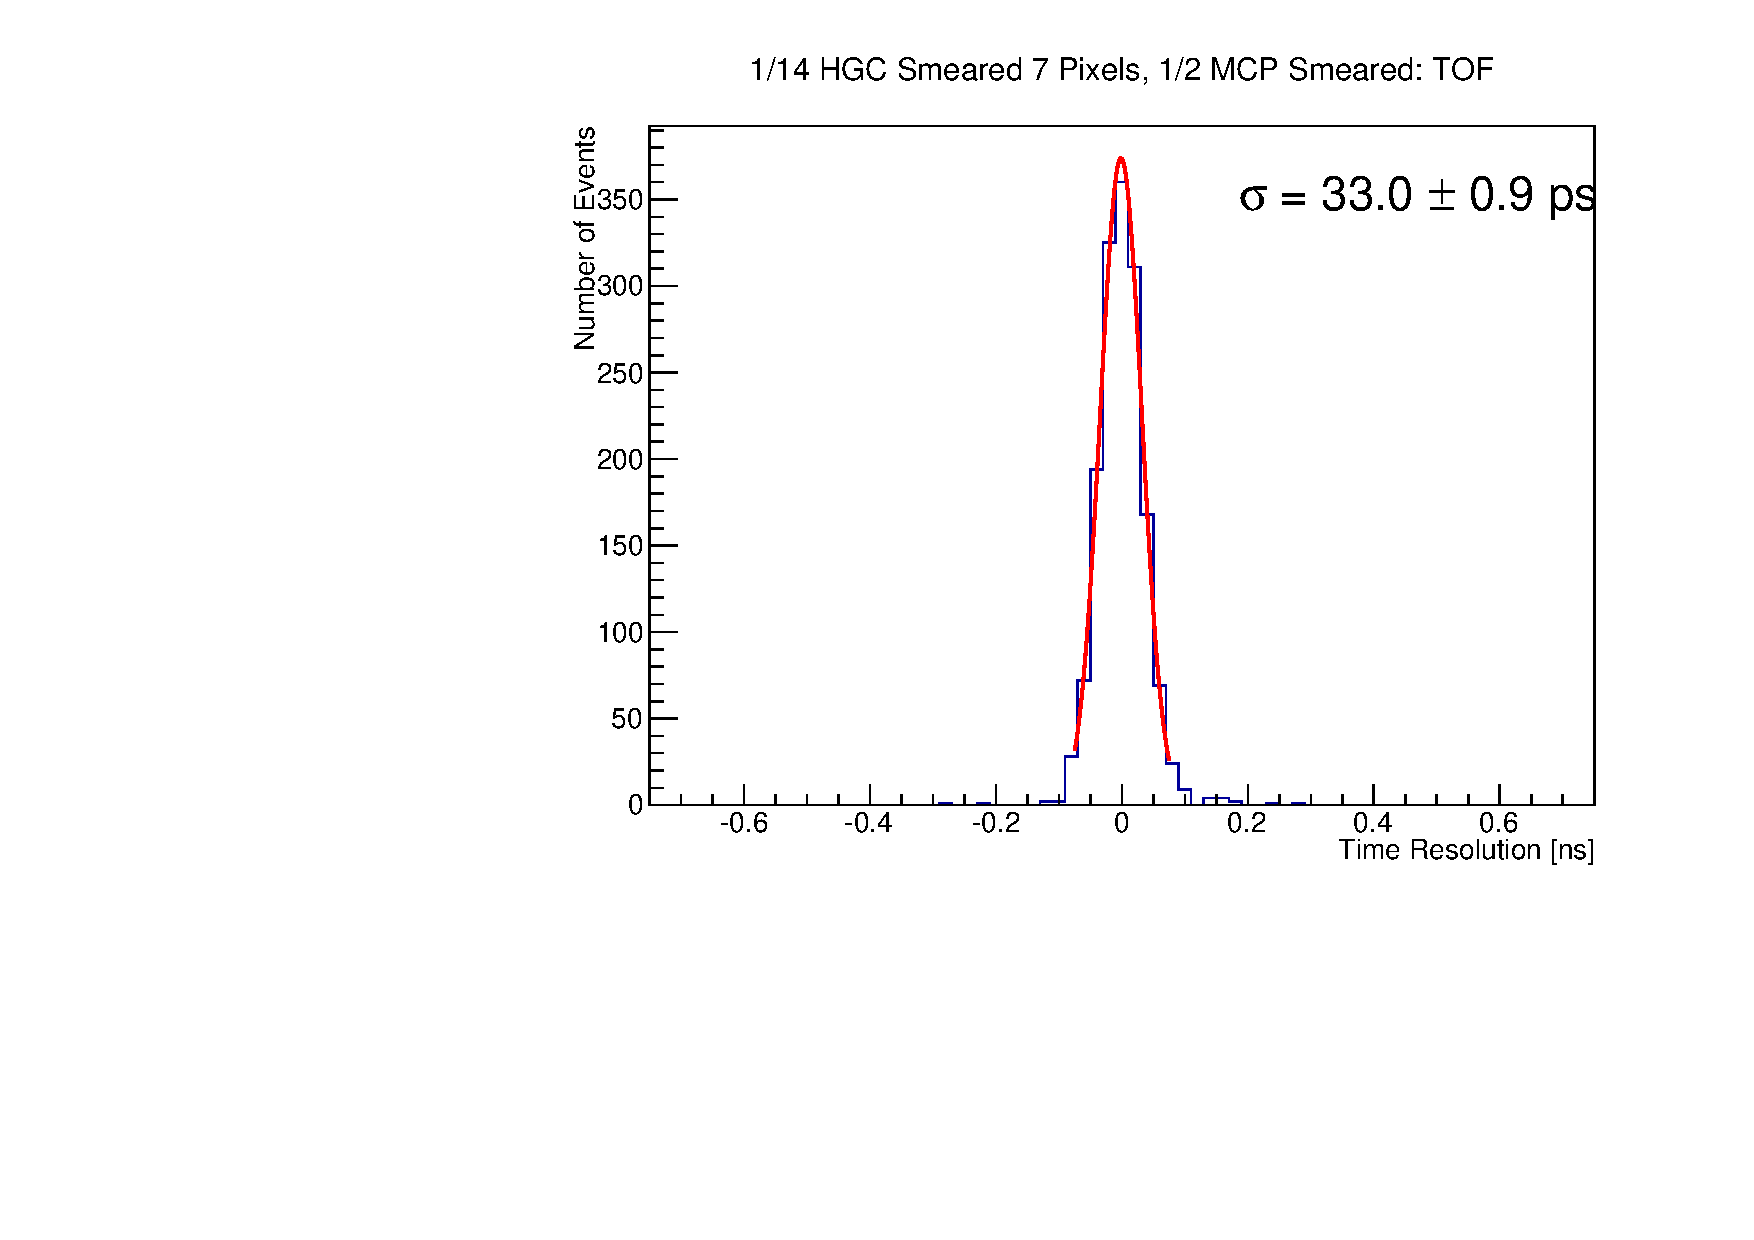
\includegraphics[width=\linewidth]{deltaT_PicoSilEqual_MCP_Equal_BothSmear50.pdf}
	\caption{TOF histogram: $\Delta t_{HGC_{Equal}}$ and $\Delta t_{Photonis}$ each weighted $\frac{1}{2}$.}
	\label{fig:50ps_HGCequal_MCP}
\end{minipage}
\end{figure*}

The Photonis MCP-PMT has also been smeared, but only by 45 ps in order to simulate a second, combined HGC layer in the longitudinal direction. 
Figures \ref{fig:50p_MCP} and \ref{fig:50ps_HGCequal_MCP} show the smeared Photonis TOF histogram and the equally-weighted TOF histogram of the Photonis and entire HGC layer.

\begin{figure}[!htbp]
	\centering
	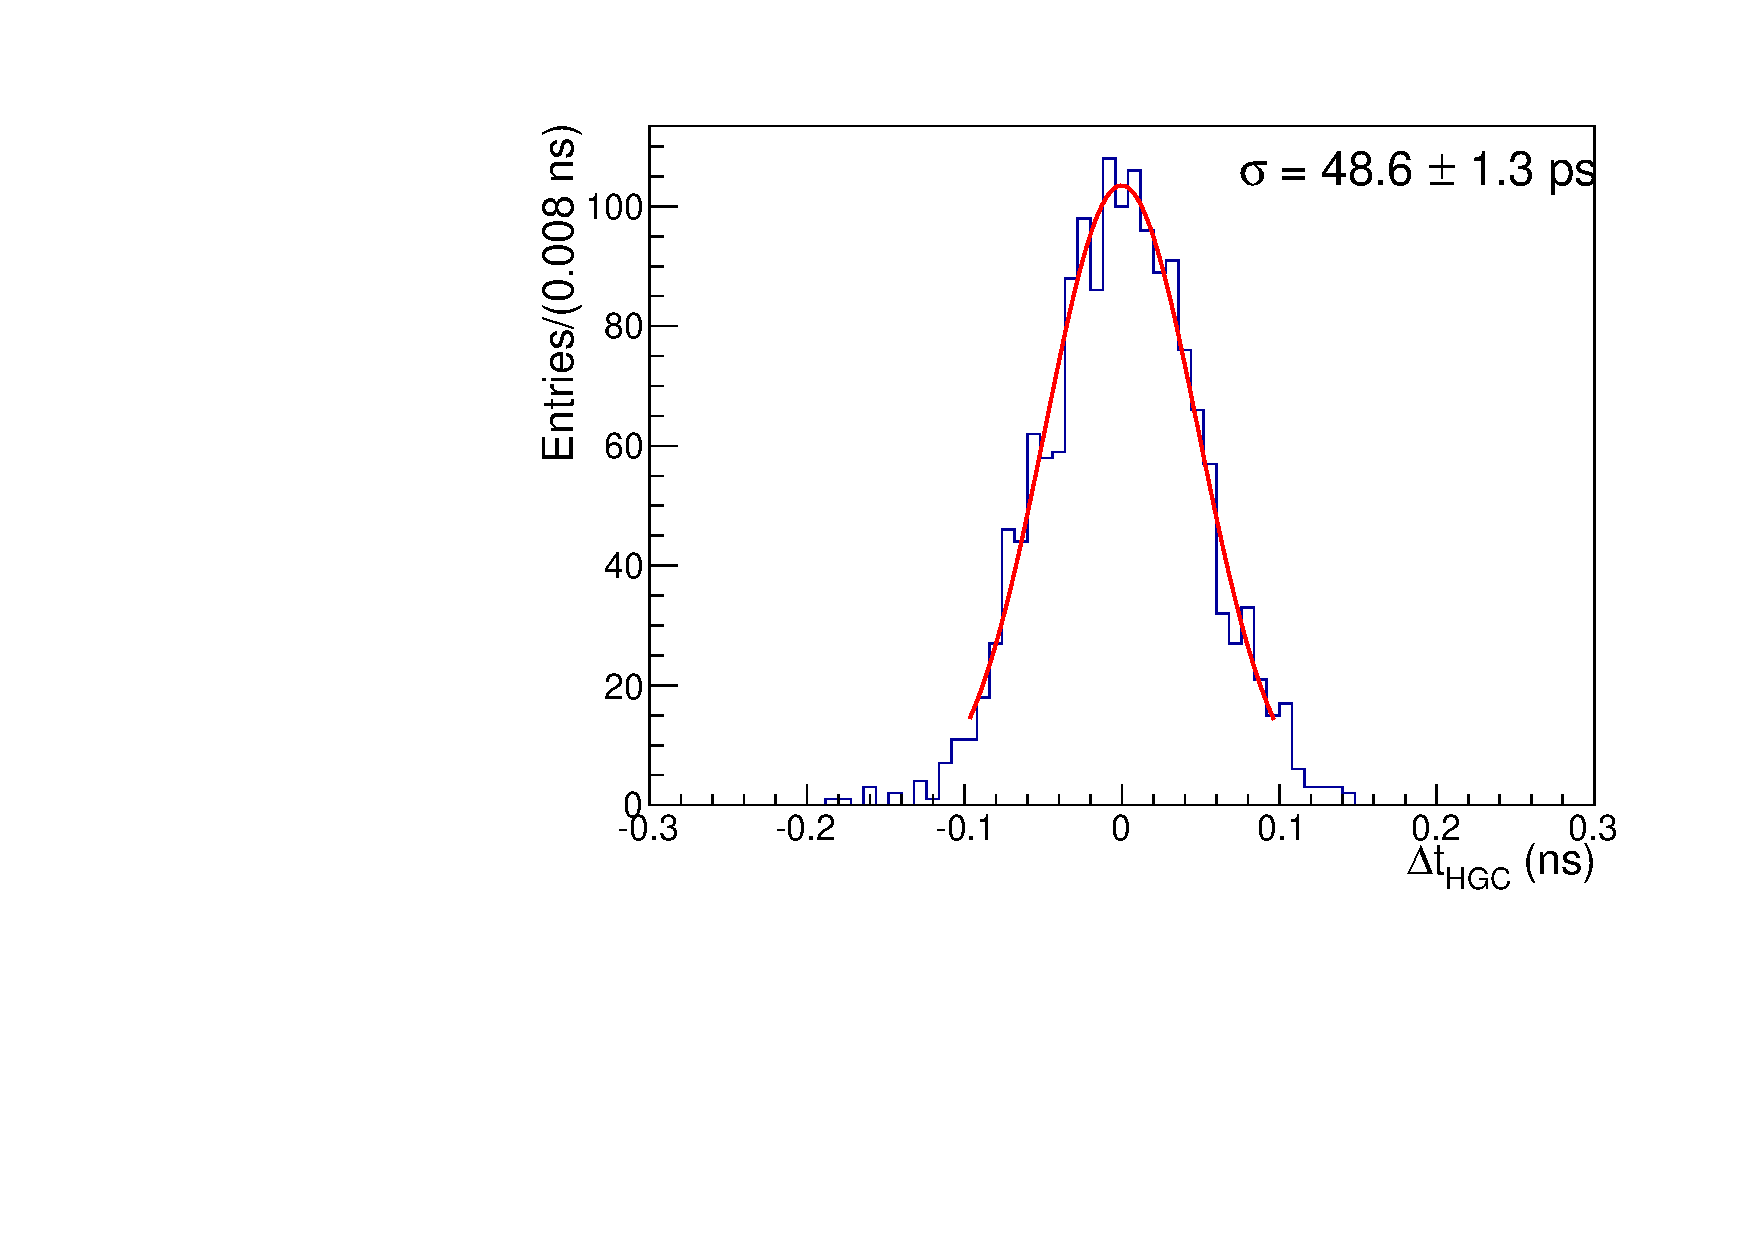
\includegraphics[width=\linewidth]{deltaTPicoSilLandauChargeSmear50.pdf}
	\caption{TOF histogram of the HGC pixels combined with a charge MPV weighting.}
	\label{fig:50ps_HGCMPV}

	\centering
	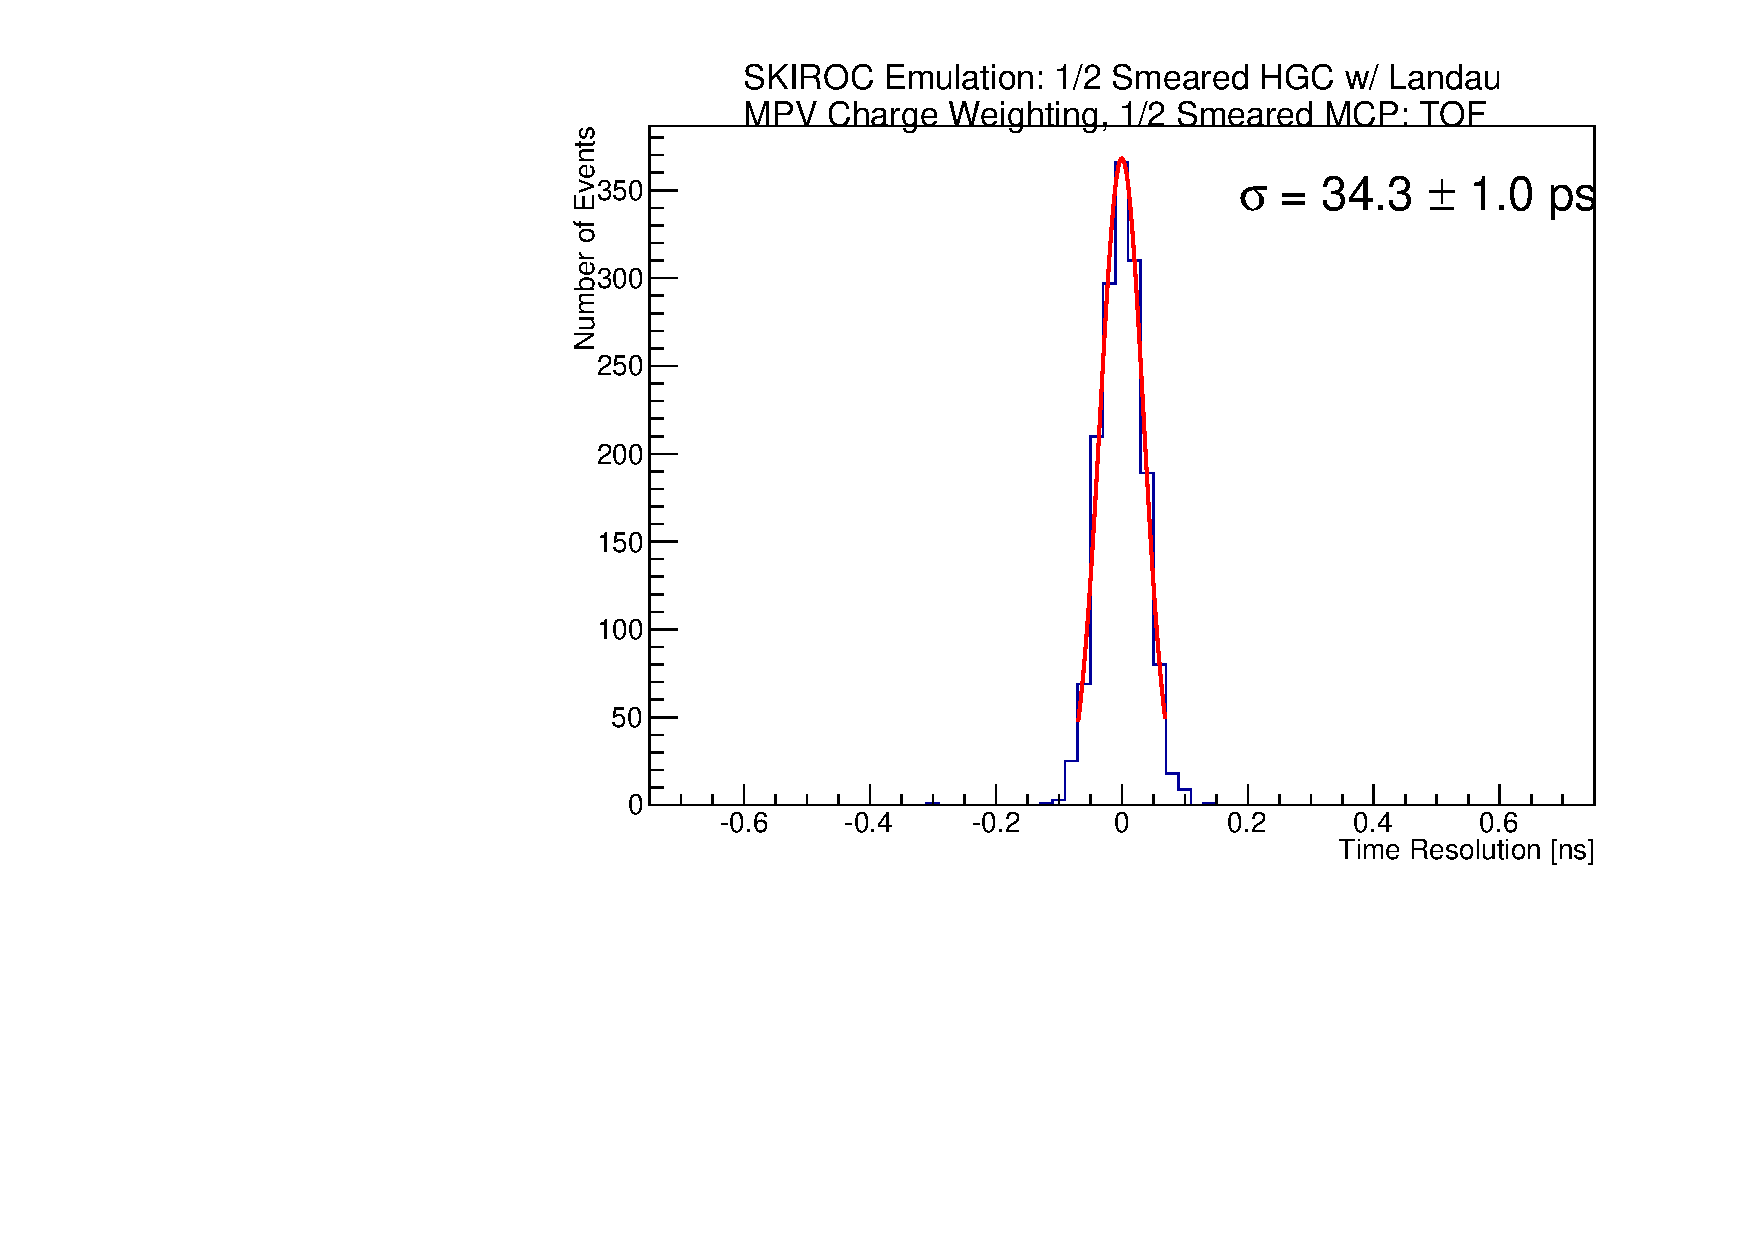
\includegraphics[width=\linewidth]{deltaT_PicoSilLandauCharge_MCP_Equal_BothSmear50.pdf}
	\caption{TOF histogram: $\Delta t_{HGC_{MPV}}$ and $\Delta t_{Photonis}$ each weighted $\frac{1}{2}$.}
	\label{fig:50ps_HGCMPV_MCP}
\end{figure}

For comparison, Figures \ref{fig:50ps_HGCMPV} and \ref{fig:50ps_HGCMPV_MCP} show the TOF histograms of the charge MPV-combined HGC layer, and of the Photonis equally weighted with the charge MPV-combined HGC layer.
Both detectors have been smeared by the same amounts as in Figures \ref{fig:50p_MCP} and \ref{fig:50ps_HGCequal_MCP}.
Charge MPV weighting is used because it is one of the better charge-weighting methods (versus event, total charge). 
Already at a smearing of 50 ps, the equal weighting of all pixels within the HGC layer appears to be slightly better than the charge MPV weighting, both for the HGC histogram and the HGC-Photonis histogram. 

\subsubsection{Add Pixels Individually: Exclude Center Pixel}
\begin{figure*}[!htbp]
\centering
	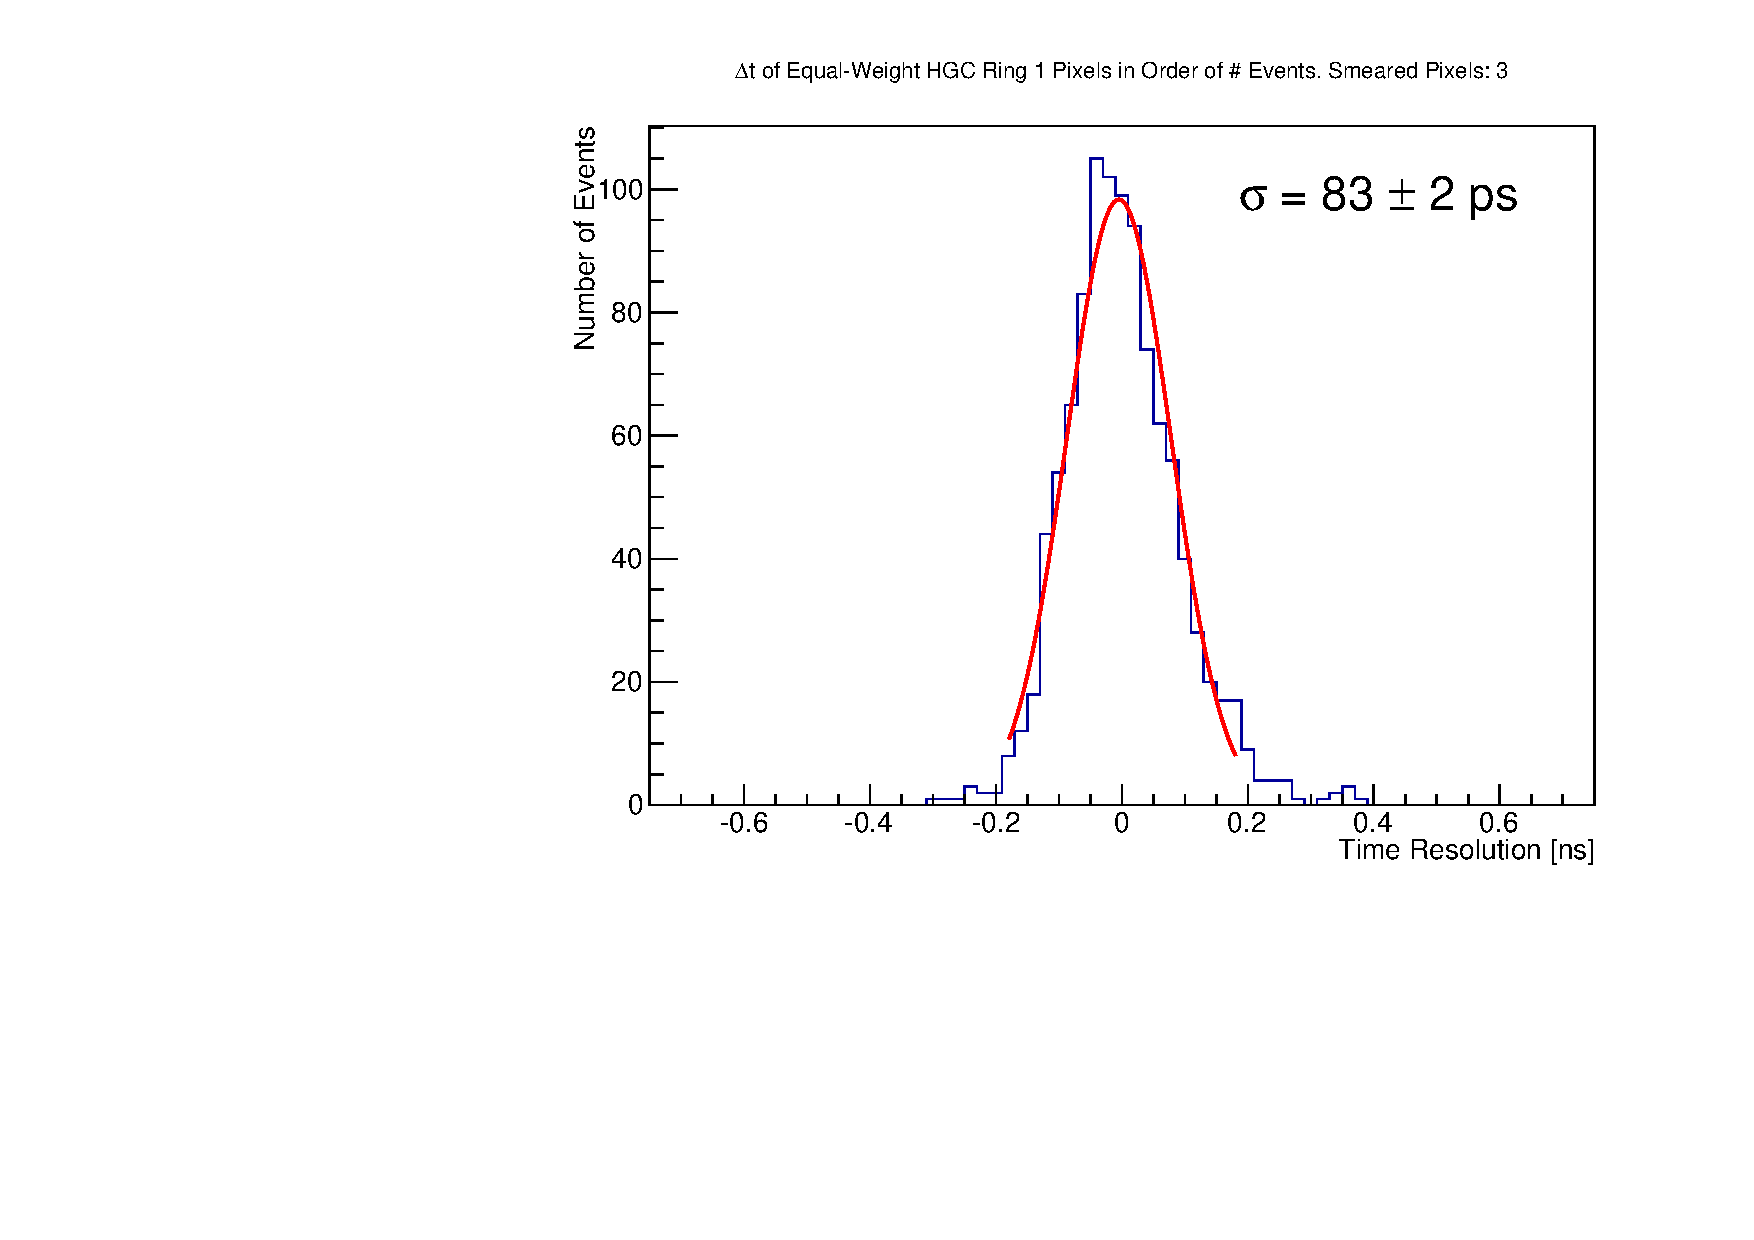
\includegraphics[width=0.32\textwidth]{SKIROC_1_Pixels_NoCenter50.pdf}
	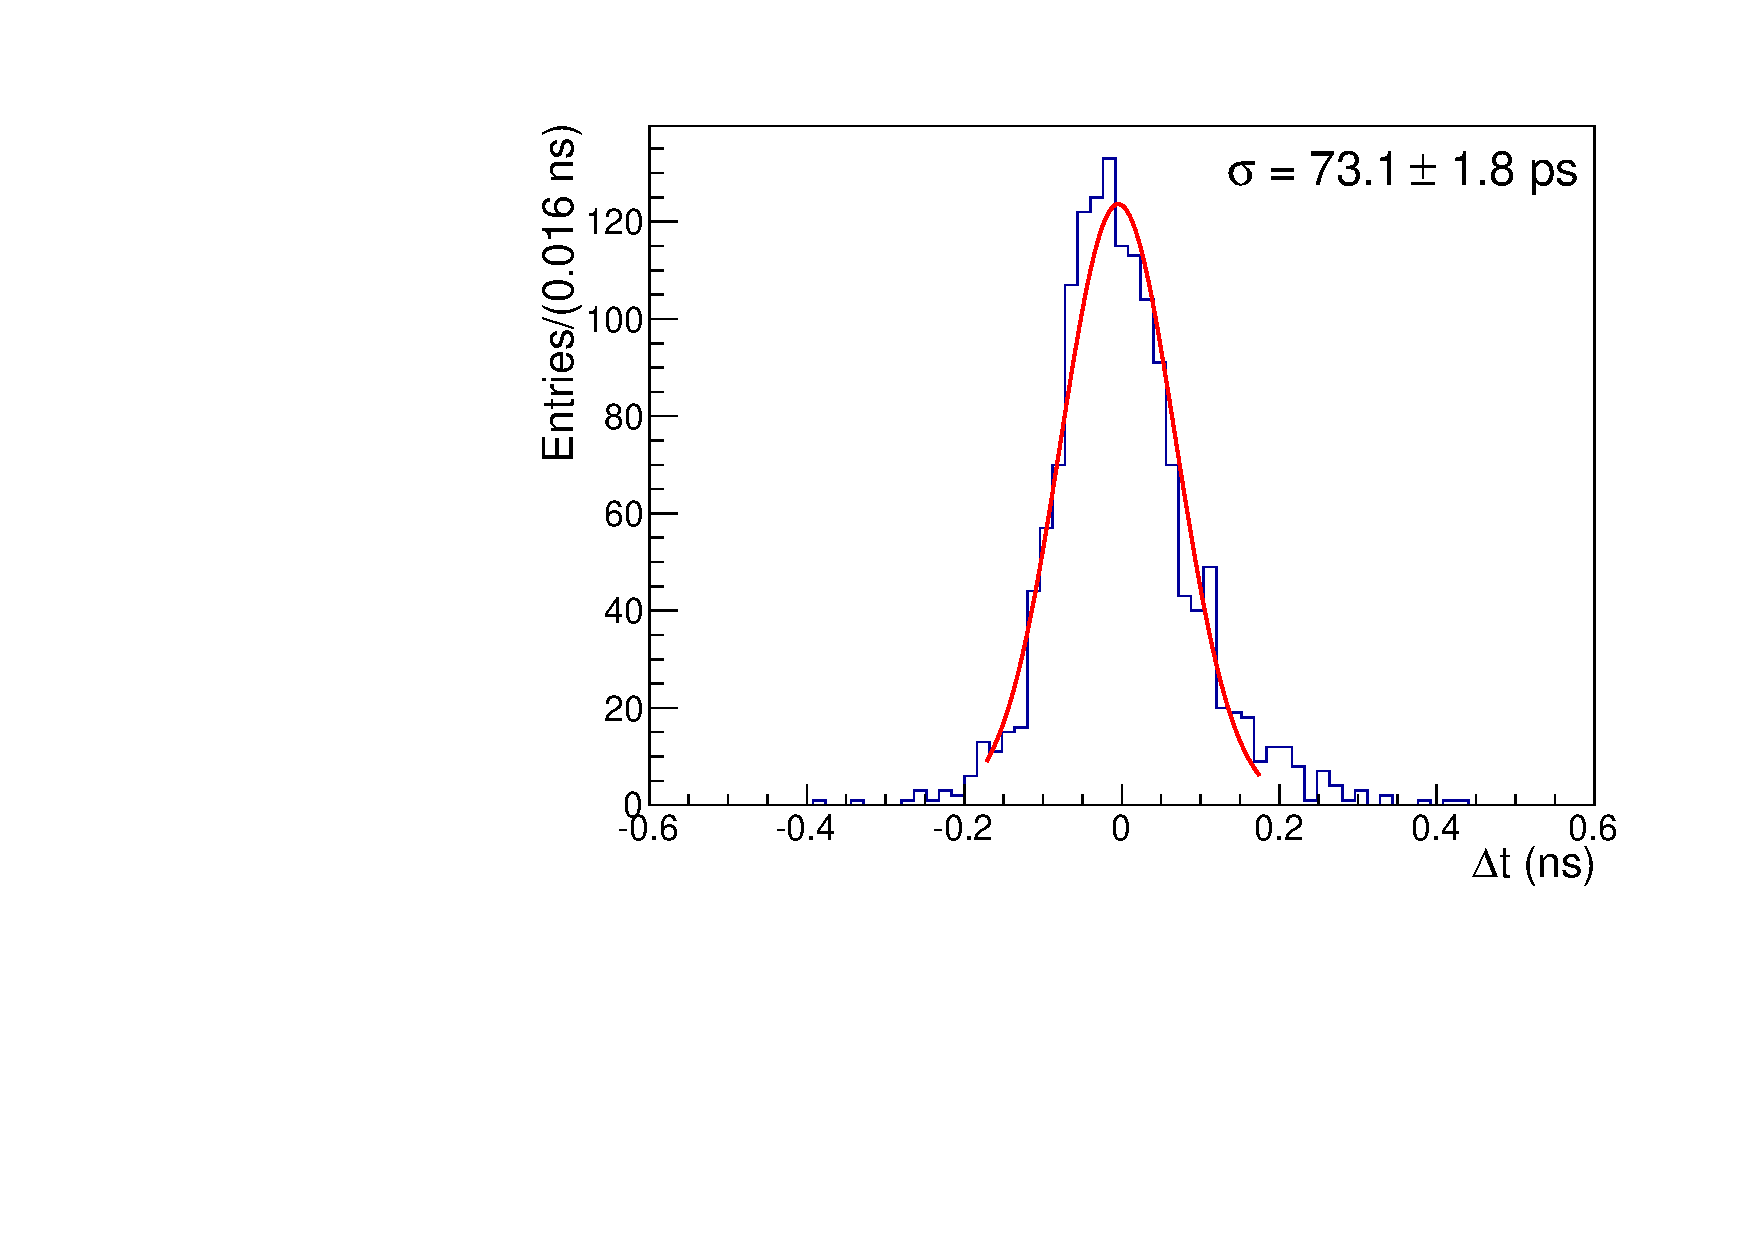
\includegraphics[width=0.32\textwidth]{SKIROC_2_Pixels_NoCenter50.pdf}
	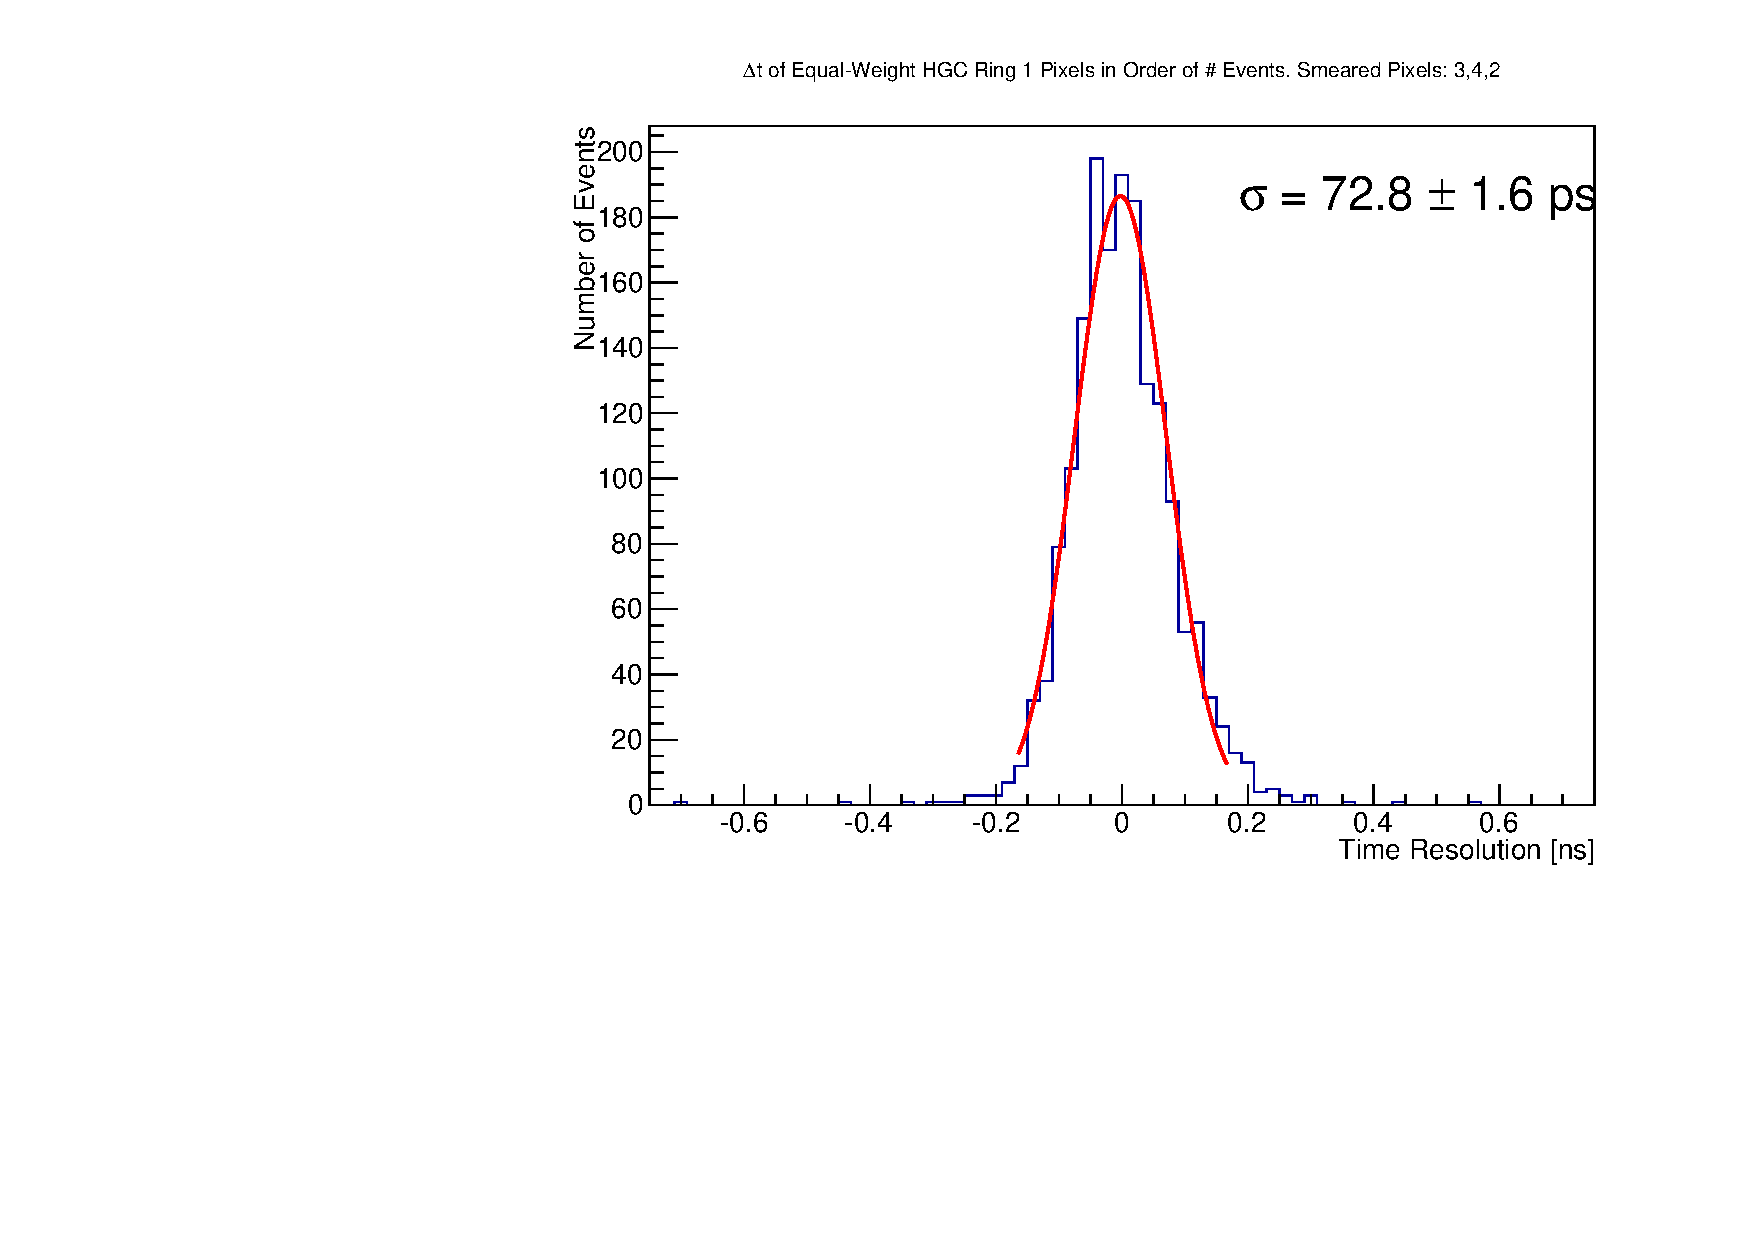
\includegraphics[width=0.32\textwidth]{SKIROC_3_Pixels_NoCenter50.pdf}

	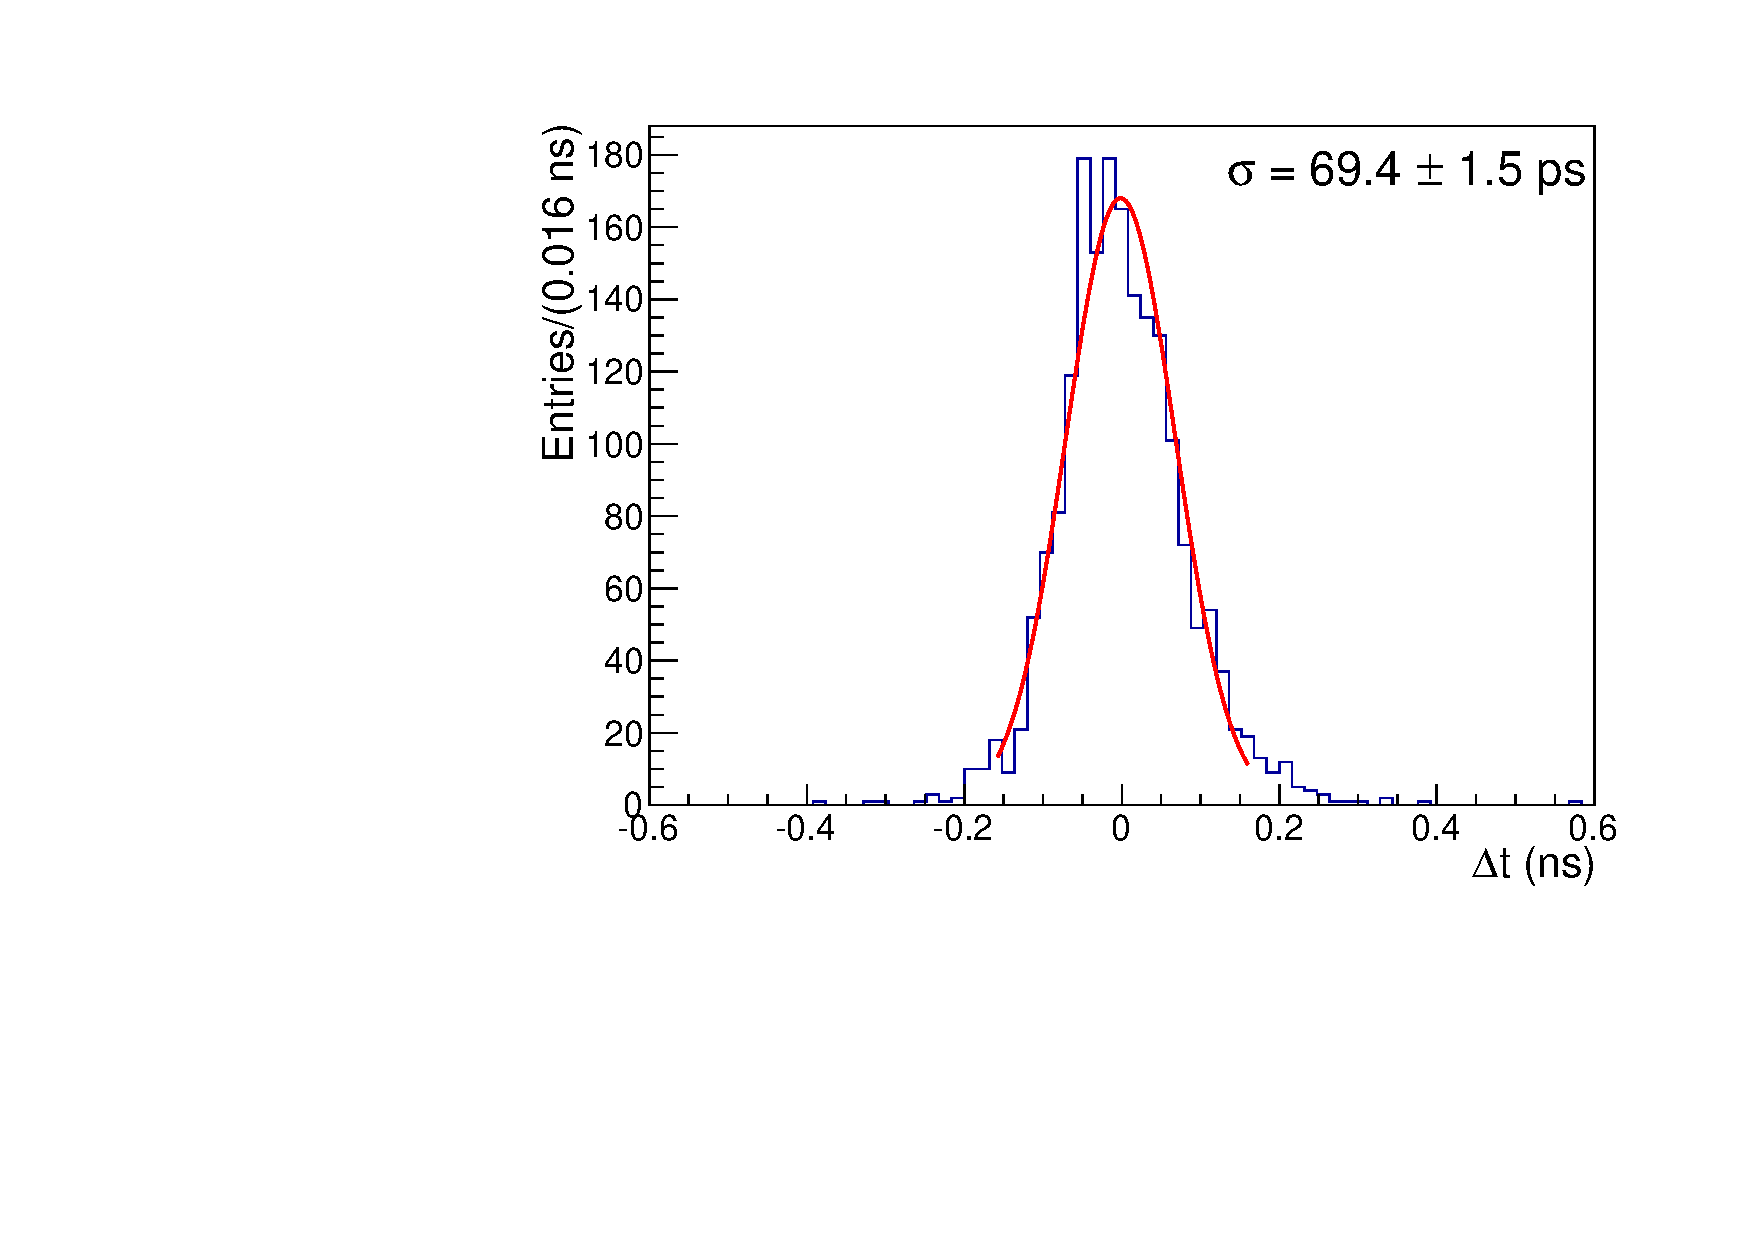
\includegraphics[width=0.32\textwidth]{SKIROC_4_Pixels_NoCenter50.pdf}
	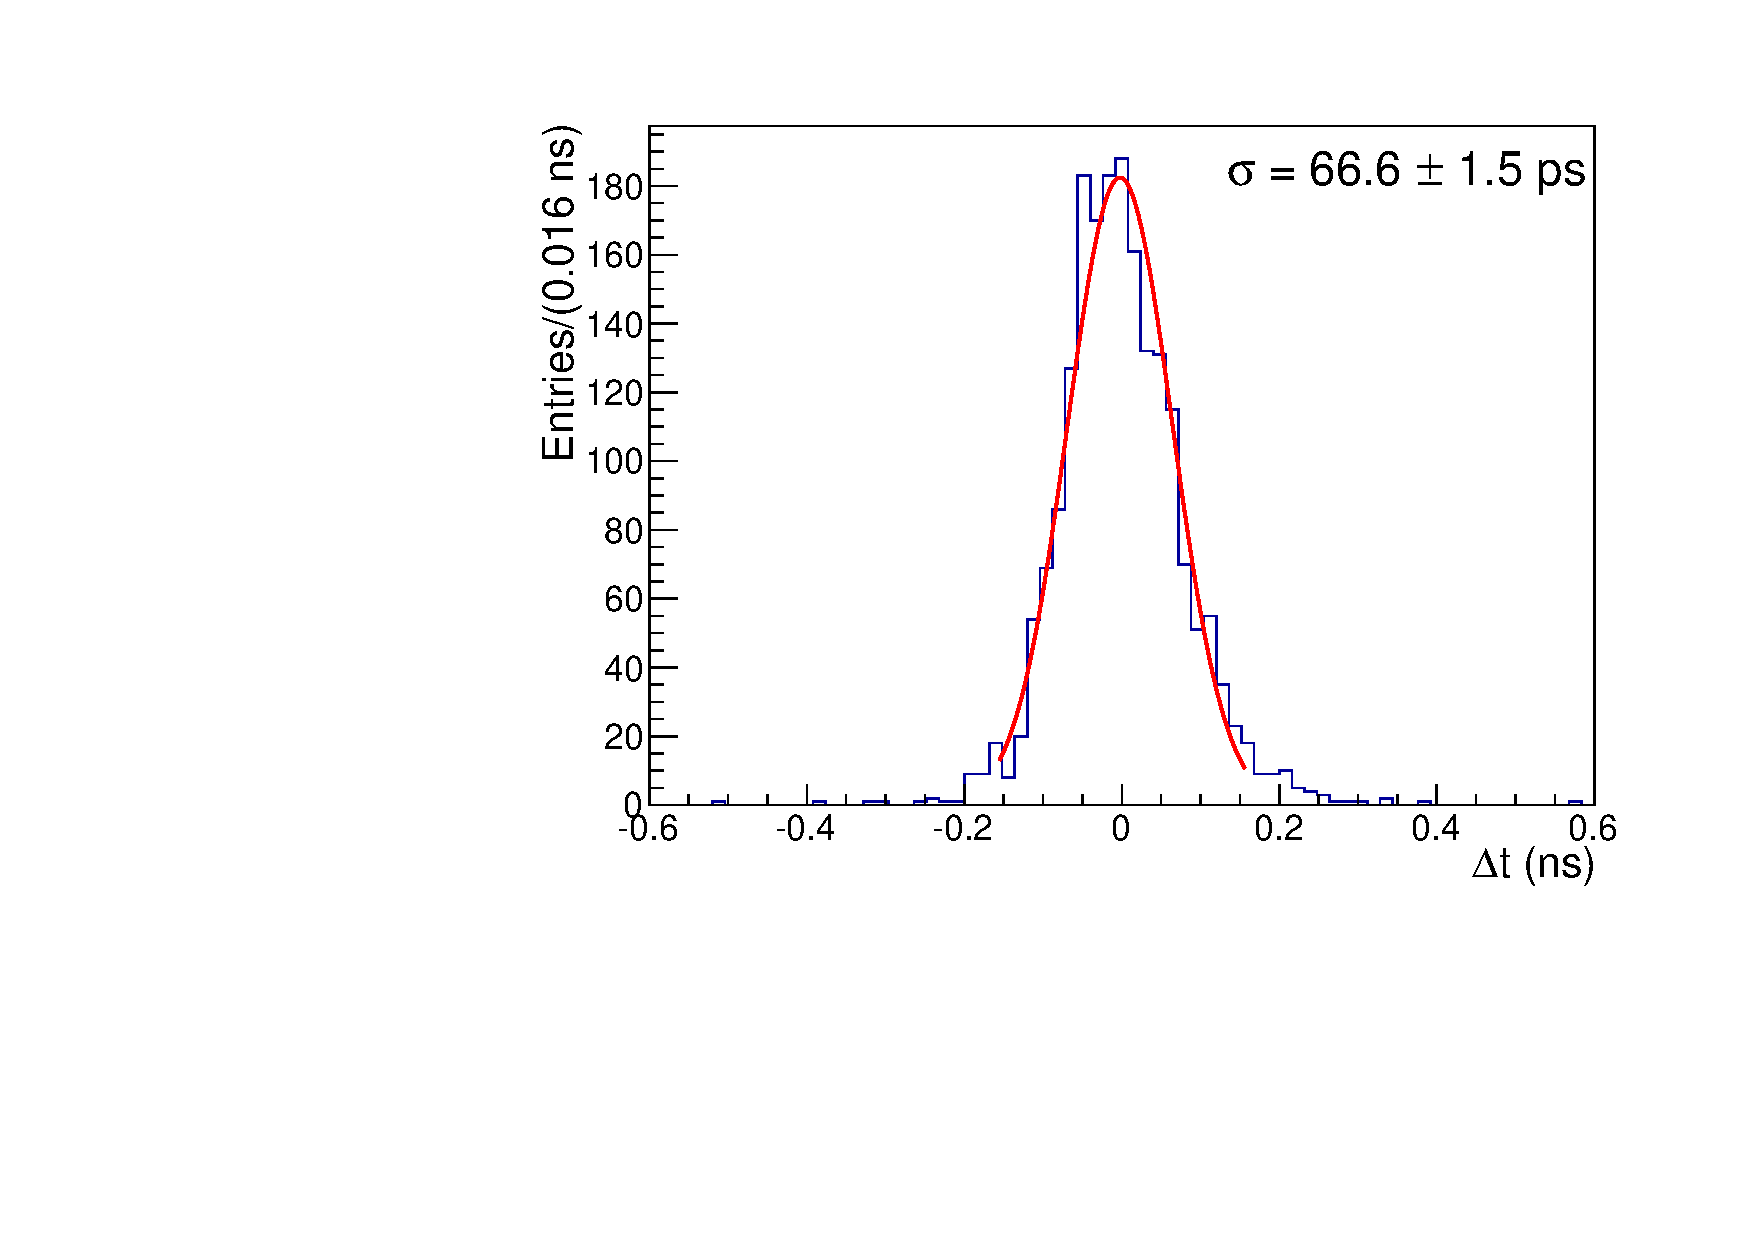
\includegraphics[width=0.32\textwidth]{SKIROC_5_Pixels_NoCenter50.pdf}
	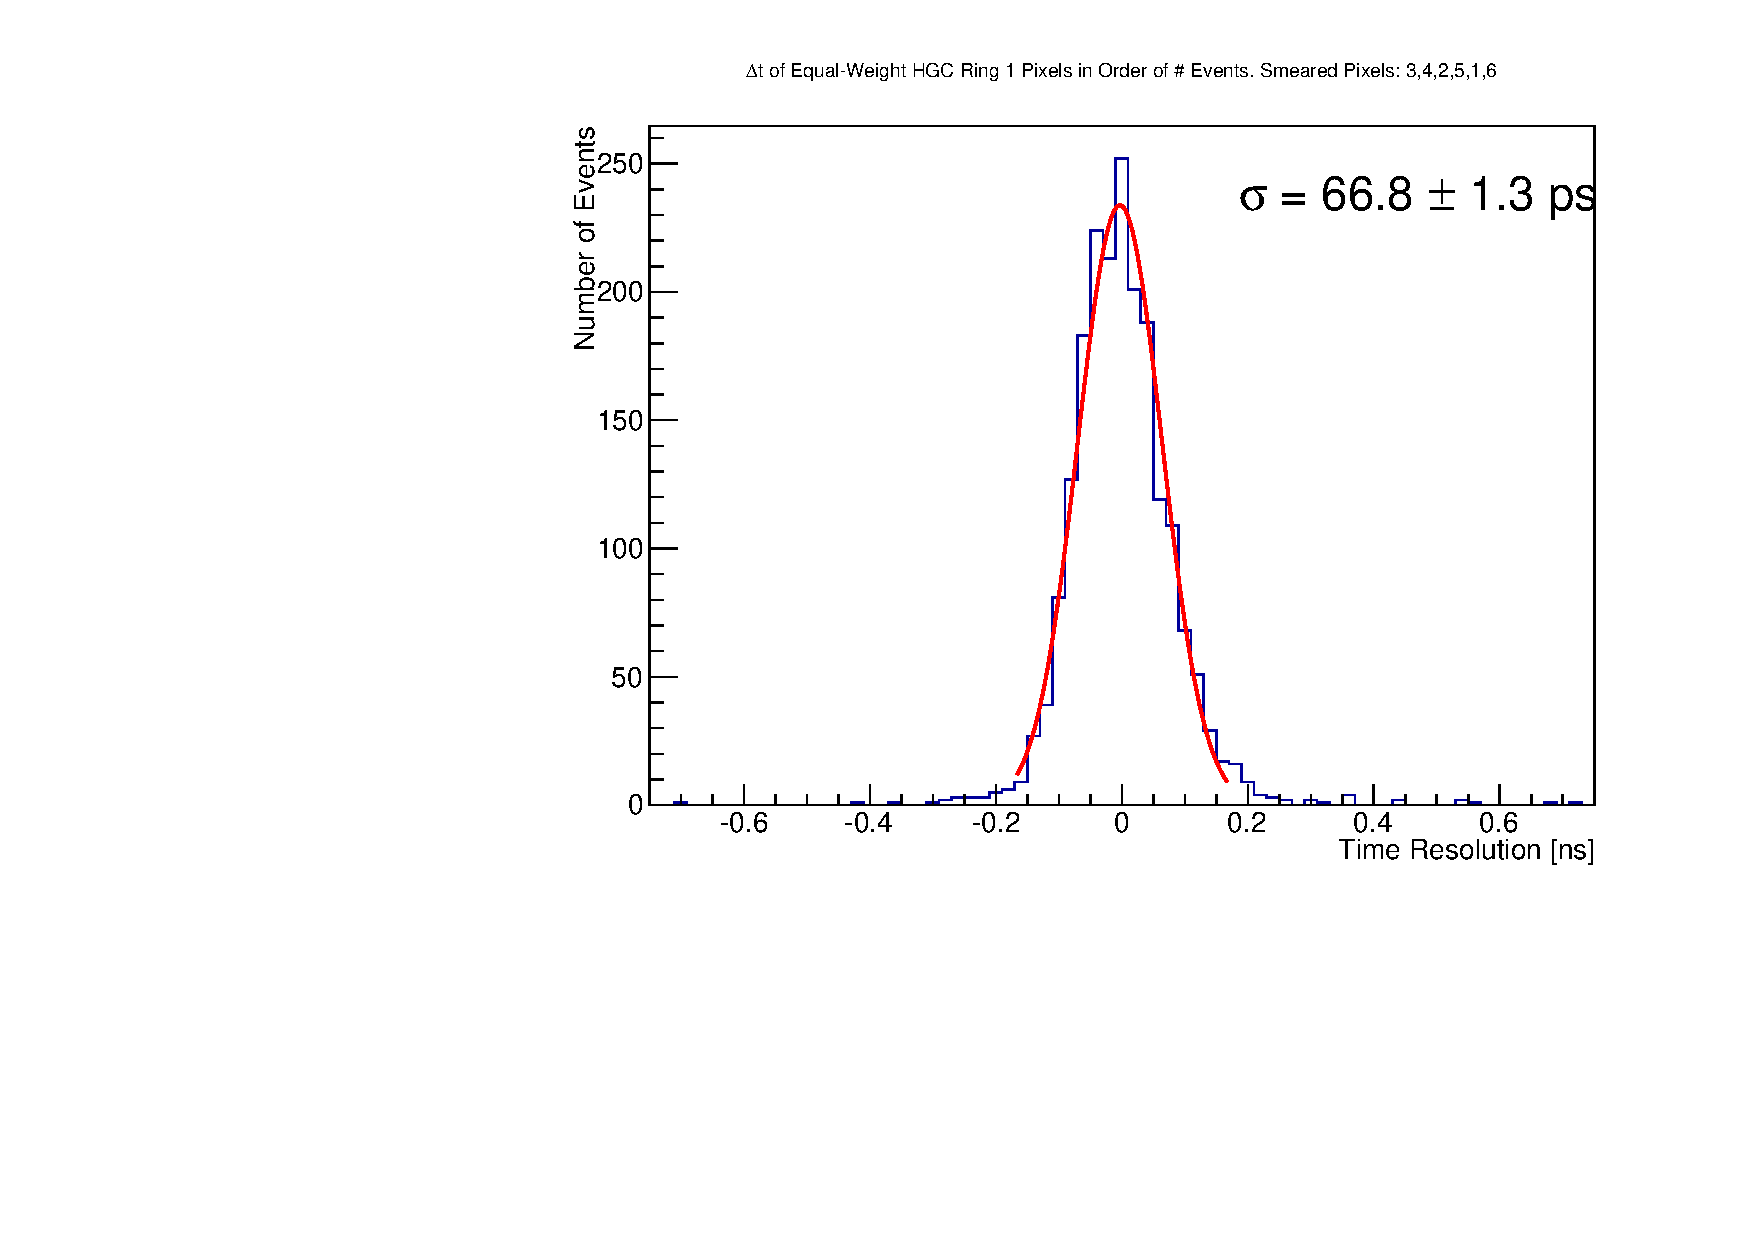
\includegraphics[width=0.32\textwidth]{SKIROC_6_Pixels_NoCenter50.pdf}
	\caption{Adding ring pixels in decreasing events order.
		Each has been smeared by 50 ps.}
	\label{fig:50psAll_NoCenter}
\end{figure*}

The improvement in the previous section is not good enough to reach the pre-smearing time resolutions. 
Perhaps combining the ring pixels without incorporating the center pixel will show a bigger improvement ($\sigma_i-\sigma_f$) due to combining detectors of similar time resolution. 
Figure \ref{fig:50psAll_NoCenter} shows the addition of each smeared pixel using an equal weighting method.
Even though the initial and final TOF histogram time resolutions are worse than when incorporating the center pixel, the improvement is about twice as large.

\subsection{500 ps Smear}
\subsubsection{Add Pixels Individually: All Pixels}
In order to illustrate the strength of the equal weighting method over charge-based methods at high smear values, a 500 ps Gaussian smearing is applied to each pixel.
Here the charge should have no correlation to the time resolution of each detector.
Additionally, the center pixel should have the same weighting factor as any other pixel, since it has equally as bad of a resolution.

\begin{figure*}[!htbp]
\centering
	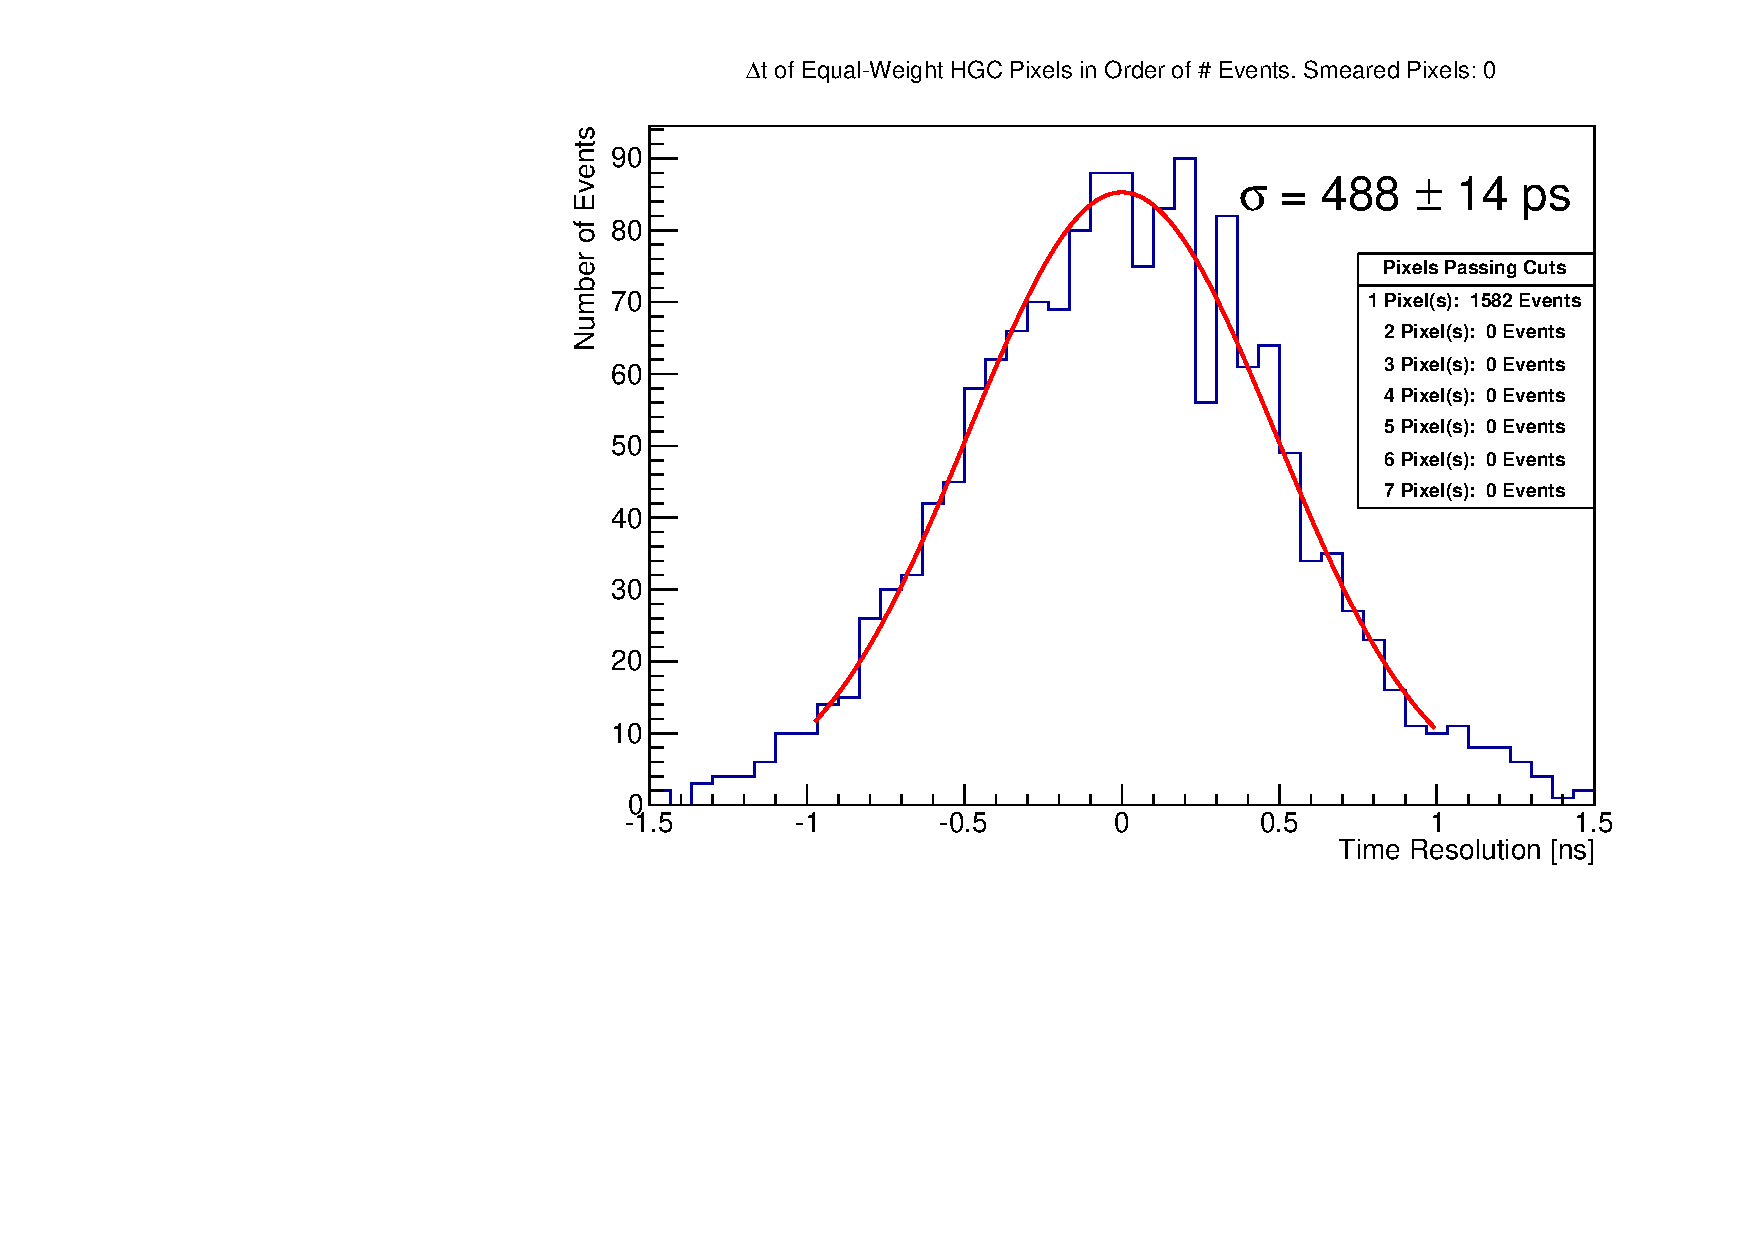
\includegraphics[width=0.35\textwidth]{SKIROC_1_Pixels500.pdf}
	\includegraphics[width=0.35\textwidth]{SKIROC_2_Pixels500.pdf}
	
	\includegraphics[width=0.32\textwidth]{SKIROC_3_Pixels500.pdf}
	\includegraphics[width=0.32\textwidth]{SKIROC_4_Pixels500.pdf}
	\includegraphics[width=0.32\textwidth]{SKIROC_5_Pixels500.pdf}
	
	\includegraphics[width=0.35\textwidth]{SKIROC_6_Pixels500.pdf}
	\includegraphics[width=0.35\textwidth]{SKIROC_7_Pixels500.pdf}
	\caption{Adding in pixels in decreasing events order.
		Each has been smeared by 500 ps.}
	\label{fig:500psAll}
\end{figure*}

Figure \ref{fig:500psAll} shows the addition of each smeared pixel using an equal weighting method. 
Note that the 7 pixel combination has between 2 and 3 pixels pass the cuts on average. 
The improvement from the initial time resolution of 500 ps is roughly 1.5, or $\sqrt{2.3}$.
Mathematically, combining different Gaussians with equal $\sigma$'s, we expect (propagating errors)

\[
\dfrac{A+B+...}{n}
\rightarrow
\frac{1}{n}\sqrt{\sigma_A^2+\sigma_B^2+...} =
\frac{1}{n}\sqrt{n \sigma^2} =
\frac{1}{\sqrt{n}} \sigma = 
\sigma'
\]

\centerline{
a $\dfrac{1}{\sqrt{n}}$ improvement in the time resolution.
}

This is close to the results above. 
Note that this improvement was not seen in the 50 ps smearing because the initial $\sigma$ of the distributions were not equal/similar.

In order to simulate another HGC layer, the Photonis MCP-PMT was smeared to 330 ps and combined with the TOF values that were used to populate the final histogram in Figure \ref{fig:500psAll}. 
The Photonis TOF and combined TOF histograms are given in Figures \ref{fig:500psMCP} and \ref{fig:500psHGCMCP}. 
The initial 500 ps resolution was improved to around 240 ps. 

\begin{figure*}[!htbp]
\centering
\begin{minipage}[t]{0.49\textwidth}
	\includegraphics[width=\linewidth]{deltaTMCPSmear500.pdf}
	\caption{TOF histogram for Photonis MCP-PMT smeared to 330 ps.}
	\label{fig:500psMCP}
\end{minipage} \hfill
\begin{minipage}[t]{0.49\textwidth}
	\includegraphics[width=\linewidth]{deltaT_PicoSilEqual_MCP_Equal_BothSmear500.pdf}
	\caption{TOF histogram, equally weighting smeared HGC layer and Photonis.}
	\label{fig:500psHGCMCP}
\end{minipage}
\end{figure*}

\subsubsection{Add Pixels Individually: Exclude Center Pixel}
As it was for the 50 ps simulation, computing the combined TOF histogram using just the ring pixels may be insightful.
Figure \ref{fig:500psAll_NoCenter} shows the time resolution improves from about 500 ps to approximately 370 ps. 
The upshot is that the center pixel is not necessary for the time resolution to improve.
However if the center pixel initially has a much better time resolution then the improvement will be limited.

\begin{figure*}[!htbp]
\centering
	\includegraphics[width=0.32\textwidth]{SKIROC_1_Pixels_NoCenter500.pdf}
	\includegraphics[width=0.32\textwidth]{SKIROC_2_Pixels_NoCenter500.pdf}
	\includegraphics[width=0.32\textwidth]{SKIROC_3_Pixels_NoCenter500.pdf}

	\includegraphics[width=0.32\textwidth]{SKIROC_4_Pixels_NoCenter500.pdf}
	\includegraphics[width=0.32\textwidth]{SKIROC_5_Pixels_NoCenter500.pdf}
	\includegraphics[width=0.32\textwidth]{SKIROC_6_Pixels_NoCenter500.pdf}
	\caption{Adding ring pixels in decreasing events order.
		Each has been smeared by 500 ps.}
	\label{fig:500psAll_NoCenter}
\end{figure*}


\begin{table*}
\centering
\begin{tabular}{ |c|c|c|c|c|c|c|c|c|c| }
\hline
%%% HEADERS:
\multicolumn{1}{|p{1.2cm}|}{\centering Beam\\Energy\\(GeV)}
& \multicolumn{1}{|p{1.5cm}|}{\centering 1st\\ Absorber\\Thickness ($X_0$)}
& \multicolumn{1}{|p{1.5cm}|}{\centering Space b/t\\Absorber \\and HGC \\(mm)}
& \multicolumn{1}{|p{1cm}|}{\centering Abs-\\orber \\Type}
& \multicolumn{1}{|p{1.6cm}|}{\centering 2nd \\Absorber \\Thickness ($X_0$)}
& \multicolumn{1}{|p{1.8cm}|}{\centering HGC\\Center}
& \multicolumn{1}{|p{1.8cm}|}{\centering HGC:\\MPV}
& \multicolumn{1}{|p{1.8cm}|}{\centering 1-ch \\Photonis}
& \multicolumn{1}{|p{1.8cm}|}{\centering Center + \\Photonis: \\Equal}
& \multicolumn{1}{|p{1.8cm}|}{\centering (HGC:MPV) \\+ Photonis: \\Equal}
\\ \hline
%%% DATA:
32 & 6 & 3-4 & Pb & 0 & 16.1 $\pm$ 0.3 ps & 15.9 $\pm$ 0.3 ps & 13.9 $\pm$ 0.2 ps & 12.2 $\pm$ 0.2 ps & 12.4 $\pm$ 0.3 ps 
\\ \hline
32 & 6 & 10 & Pb & 0 & 18.3 $\pm$ 0.4 ps & 17.6 $\pm$ 0.4 ps & 14.1 $\pm$ 0.3 ps & 13.2 $\pm$ 0.3 ps & 13.6 $\pm$ 0.3 ps 
\\ \hline
32 & 6 & 34 & Pb & 0 & 24.9 $\pm$ 0.5 ps & 30.3 $\pm$ 0.5 ps & 15.6 $\pm$ 0.4 ps & 15.3 $\pm$ 0.3 ps & 17.9 $\pm$ 0.3 ps 
\\ \hline
32 & 6 & 1 & W & 0 & 15.9 $\pm$ 0.4 ps & 15.5 $\pm$ 0.4 ps & 13.4 $\pm$ 0.3 ps & 11.4 $\pm$ 0.3 ps & 11.4 $\pm$ 0.3 ps 
\\ \hline
32 & 6 & 10 & W & 0 & 18.4 $\pm$ 0.6 ps & 19.6 $\pm$ 0.5 ps & 13.9 $\pm$ 0.4 ps & 12.3 $\pm$ 0.4 ps & 12.9 $\pm$ 0.3 ps 
\\ \hline
32 & 6 & 32 & W & 0 & 21.8 $\pm$ 0.6 ps & 21.6 $\pm$ 0.5 ps & 14.3 $\pm$ 0.5 ps & 14.4 $\pm$ 0.5 ps & 14.4 $\pm$ 0.3 ps 
\\ \hline
16 & 6 & 1 & W & 0 & 20.9 $\pm$ 0.3 ps & 20.2 $\pm$ 0.3 ps & 17.0 $\pm$ 0.2 ps & 14.4 $\pm$ 0.2 ps & 14.2 $\pm$ 0.2 ps 
\\ \hline
16 & 3 & 1 & W & 3 & 39.3 $\pm$ 0.4 ps & 38.2 $\pm$ 0.4 ps & 15.7 $\pm$ 0.2 ps & 21.9 $\pm$ 0.2 ps & 21.6 $\pm$ 0.2 ps 
\\ \hline
8 & 6 & 1 & W & 0 & 30.5 $\pm$ 0.3 ps & 31.9 $\pm$ 0.4 ps & 24.3 $\pm$ 0.3 ps & 21.4 $\pm$ 0.2 ps & 21.9 $\pm$ 0.2 ps 
\\ \hline
8 & 3 & 1 & W & 3 & 44.0 $\pm$ 0.5 ps & 44.7 $\pm$ 0.5 ps & 19.6 $\pm$ 0.2 ps & 25.4 $\pm$ 0.3 ps & 25.6 $\pm$ 0.3 ps 
\\ \hline
\end{tabular}
	\caption{Time resolution results for different configurations.}
	\label{table:results}
\end{table*}
% helpful: http://ericwood.org/excel2latex/

\section{Time of Flight Between HGC and Photonis}
Everything in the previous two sections has been generated from a 32 GeV electron beam run, with 6 $X_0$ of tungsten absorber 1 mm in front of the HGC layer. 
Different results are obtained when running the analysis code to generate time-of-flight histograms for other experimental configurations.
Table \ref{table:results} shows $\sigma$ values from different combinations for a few different runs.
From the table, some trends are clear. 
When the beam energy increases, the time resolutions improve. 
Additionally, when the gap between the absorber and the HGC layer increases, the time resolutions get worse.

For the 2 runs with a second absorber in the table, the 6 $X_0$ of absorber in front of the silicon/HGC layer gets replaced with 3 $X_0$ in front and 3 $X_0$ behind it (but still in front of the Photonis and Photek).
The HGC time resolution gets significantly worse in these configurations.
Additionally, combining the detectors with equal weighting results in a time resolution noticeably \textit{worse} than just the Photonis MCP-PMT time resolution.
A possible explanation for this phenomena is that the particle shower only developed/spread out \textit{after} passing through the HGC layer, which smeared the normal distribution of times from the HGC pixels. 
In this case, the higher time resolutions would be attributed to the 3 $X_0$ behind the HGC layer.

A way to see if the 3 $X_0$ plays a role in the higher time resolutions is to compute a different time-of-flight.
Previously the TOF values calculated were either from an HGC pixel to the Photek, or from the Photonis to the Photek.
However, if a TOF from the HGC layer to the Photonis increases significantly from the first runs in the table to the last 2 runs, then the above assertion may gain some ground.

\begin{figure}[!htbp]
\centering
	\includegraphics[width=\linewidth]{deltaT_PicoSil_vs_MCP_TotalCharge_16gev.pdf}
    
	\includegraphics[width=\linewidth]{deltaT_PicoSil_vs_MCP_TotalCharge_16gevDelay.pdf}
	\caption{The TOF histograms from the HGC layer to the Photonis for 16 GeV electron beams.
	The pixel TOF values were combined with total charge weighting.
	The top plot has 6 $X_0$ of tungsten absorber in front of the HGC layer.
	The bottom plot has 3 $X_0$ on either side of the HGC layer.}
	\label{fig:HGCvsMCP}
\end{figure}

From Figure \ref{fig:HGCvsMCP}, it is clear that the different absorber arrangement is the cause of the worse time resolution values.
However, it is not yet possible to attribute this effect to the 3 $X_0$ in front of the HGC, because it may be the the 3 $X_0$ behind the HGC.
Table \ref{table:vs} has the new TOF $\sigma$ values for most of the runs in Table \ref{table:results}.


\begin{table*}
\centering
\begin{tabular}{ |c|c|c|c|c|c|c| }
\hline
%%% HEADERS:
\multicolumn{1}{|p{1.5cm}|}{\centering Beam Energy\\(GeV)}
& \multicolumn{1}{|p{1.7cm}|}{\centering 1st\\ Absorber\\Thickness ($X_0$)}
& \multicolumn{1}{|p{1.8cm}|}{\centering Space b/t\\Absorber \\and HGC \\(mm)}
& \multicolumn{1}{|p{1.6cm}|}{\centering Absorber \\Type}
& \multicolumn{1}{|p{1.7cm}|}{\centering 2nd \\Absorber \\Thickness ($X_0$)}
& \multicolumn{1}{|p{1.8cm}|}{\centering Event\\Charge\\Weight}
& \multicolumn{1}{|p{1.8cm}|}{\centering Total\\Charge\\Weight}
\\ \hline
%%% DATA:
32 & 6 & 3-4 & Pb & 0 & 18.4 ps & 18.5 ps
\\ \hline
32 & 6 & 10 & Pb & 0 & 20.4 ps & 21.2 ps
\\ \hline
32 & 6 & 34 & Pb & 0 & 34.3 ps & 28.2 ps 
\\ \hline
32 & 6 & 1 & W & 0 & 17.9 ps & 18.7 ps
\\ \hline
16 & 6 & 1 & W & 0 & 25.0  ps & 24.7 ps
\\ \hline
16 & 3 & 1 & W & 3 & 39.8 ps & 41.5 ps
\\ \hline
8 & 6 & 1 & W & 0 & 39.9 ps & 38.4 ps
\\ \hline
8 & 3 & 1 & W & 3 & 49.5 ps & 49.3 ps
\\ \hline
\end{tabular}
	\caption{TOF results from the HGC layer to the Photonis for different configurations.
	Combined by HGC event and total charge TOF weightings.
	Since the pixels are not manually smeared, there is no need for equal weighting here.}
	\label{table:vs}
\end{table*}
%%% UPDATE RESULTS IN THE TABLE


\section{Summary}
In this report, different detector combination mechanisms have been defined and compared.
Charge weighting should be used for combinations when there are large disparities in the time resolutions of the HGC pixels.
Otherwise, when there exists similar resolutions or smeared pixels, then equal weighting becomes more favorable.
Additionally, there seems to be a $\sqrt{n}$ improvement in the time resolution when, on average, n pixels with similar time resolutions pass the event selection requirements, although further analysis is necessary to fully understand this.
Lastly, the existence of absorber material behind some detectors may contribute to a worse time resolution.

The analysis code is being used for the HGC layer and Photonis MCP-PMT to look at how these time resolutions vary for different configurations (i.e. absorber type, spacing, and thickness; beam energy; etc). 


%%% FOR 1 COLUMN FIGURES:
\begin{comment}
\onecolumngrid
\begin{center}
\begin{figure}
\centering
\includegraphics[width=0.98\textwidth]{eta_phi.pdf}
\end{figure}
\end{center}
\twocolumngrid
\end{comment}

\section{Future}
Further research includes testing if equally-weighting 2 detectors gives the new time resolution value of 
$
\dfrac{1}{2} \sqrt{\sigma_a^2+\sigma_b^2}
$
, and comparing it with unequal weighting results.
Furthermore, identification of MIPs in proton runs can also be investigated. 

\section{Acknowledgments}
I would like to thank Maria Spiropulu for giving me this research opportunity. 
Additionally, much credit for this work is due to the invaluable help of Cristian Pena who provided much needed guidance, as well as Si Xie, Artur Apresyan, and Javier Duarte for assistance at Fermilab. 
Also helpful was the rest of the Caltech CMS collaboration, including but not limited to Dustin Anderson, Dorian Kcira, Jason Trevor, and the summer undergraduates doing research at Caltech.
Finally, I'd like to recognize the Caltech SFP Office and Bill Davis Fellowship for providing funds for this research.

\newpage

\nocite{*}

\bibliographystyle{apsrev4-1} % Tell bibtex which bibliography style to use
\bibliography{DanielGawerc/ref.bib} 
\end{document}
